% Options for packages loaded elsewhere
\PassOptionsToPackage{unicode}{hyperref}
\PassOptionsToPackage{hyphens}{url}
%
\documentclass[
]{book}
\usepackage{amsmath,amssymb}
\usepackage{lmodern}
\usepackage{iftex}
\ifPDFTeX
  \usepackage[T1]{fontenc}
  \usepackage[utf8]{inputenc}
  \usepackage{textcomp} % provide euro and other symbols
\else % if luatex or xetex
  \usepackage{unicode-math}
  \defaultfontfeatures{Scale=MatchLowercase}
  \defaultfontfeatures[\rmfamily]{Ligatures=TeX,Scale=1}
\fi
% Use upquote if available, for straight quotes in verbatim environments
\IfFileExists{upquote.sty}{\usepackage{upquote}}{}
\IfFileExists{microtype.sty}{% use microtype if available
  \usepackage[]{microtype}
  \UseMicrotypeSet[protrusion]{basicmath} % disable protrusion for tt fonts
}{}
\makeatletter
\@ifundefined{KOMAClassName}{% if non-KOMA class
  \IfFileExists{parskip.sty}{%
    \usepackage{parskip}
  }{% else
    \setlength{\parindent}{0pt}
    \setlength{\parskip}{6pt plus 2pt minus 1pt}}
}{% if KOMA class
  \KOMAoptions{parskip=half}}
\makeatother
\usepackage{xcolor}
\IfFileExists{xurl.sty}{\usepackage{xurl}}{} % add URL line breaks if available
\IfFileExists{bookmark.sty}{\usepackage{bookmark}}{\usepackage{hyperref}}
\hypersetup{
  pdftitle={semnova: An R package for latent repeated measures ANOVA},
  pdfauthor={Benedikt Langenberg, Jonathan L. Helm, and Axel Mayer},
  hidelinks,
  pdfcreator={LaTeX via pandoc}}
\urlstyle{same} % disable monospaced font for URLs
\usepackage{color}
\usepackage{fancyvrb}
\newcommand{\VerbBar}{|}
\newcommand{\VERB}{\Verb[commandchars=\\\{\}]}
\DefineVerbatimEnvironment{Highlighting}{Verbatim}{commandchars=\\\{\}}
% Add ',fontsize=\small' for more characters per line
\usepackage{framed}
\definecolor{shadecolor}{RGB}{248,248,248}
\newenvironment{Shaded}{\begin{snugshade}}{\end{snugshade}}
\newcommand{\AlertTok}[1]{\textcolor[rgb]{0.94,0.16,0.16}{#1}}
\newcommand{\AnnotationTok}[1]{\textcolor[rgb]{0.56,0.35,0.01}{\textbf{\textit{#1}}}}
\newcommand{\AttributeTok}[1]{\textcolor[rgb]{0.77,0.63,0.00}{#1}}
\newcommand{\BaseNTok}[1]{\textcolor[rgb]{0.00,0.00,0.81}{#1}}
\newcommand{\BuiltInTok}[1]{#1}
\newcommand{\CharTok}[1]{\textcolor[rgb]{0.31,0.60,0.02}{#1}}
\newcommand{\CommentTok}[1]{\textcolor[rgb]{0.56,0.35,0.01}{\textit{#1}}}
\newcommand{\CommentVarTok}[1]{\textcolor[rgb]{0.56,0.35,0.01}{\textbf{\textit{#1}}}}
\newcommand{\ConstantTok}[1]{\textcolor[rgb]{0.00,0.00,0.00}{#1}}
\newcommand{\ControlFlowTok}[1]{\textcolor[rgb]{0.13,0.29,0.53}{\textbf{#1}}}
\newcommand{\DataTypeTok}[1]{\textcolor[rgb]{0.13,0.29,0.53}{#1}}
\newcommand{\DecValTok}[1]{\textcolor[rgb]{0.00,0.00,0.81}{#1}}
\newcommand{\DocumentationTok}[1]{\textcolor[rgb]{0.56,0.35,0.01}{\textbf{\textit{#1}}}}
\newcommand{\ErrorTok}[1]{\textcolor[rgb]{0.64,0.00,0.00}{\textbf{#1}}}
\newcommand{\ExtensionTok}[1]{#1}
\newcommand{\FloatTok}[1]{\textcolor[rgb]{0.00,0.00,0.81}{#1}}
\newcommand{\FunctionTok}[1]{\textcolor[rgb]{0.00,0.00,0.00}{#1}}
\newcommand{\ImportTok}[1]{#1}
\newcommand{\InformationTok}[1]{\textcolor[rgb]{0.56,0.35,0.01}{\textbf{\textit{#1}}}}
\newcommand{\KeywordTok}[1]{\textcolor[rgb]{0.13,0.29,0.53}{\textbf{#1}}}
\newcommand{\NormalTok}[1]{#1}
\newcommand{\OperatorTok}[1]{\textcolor[rgb]{0.81,0.36,0.00}{\textbf{#1}}}
\newcommand{\OtherTok}[1]{\textcolor[rgb]{0.56,0.35,0.01}{#1}}
\newcommand{\PreprocessorTok}[1]{\textcolor[rgb]{0.56,0.35,0.01}{\textit{#1}}}
\newcommand{\RegionMarkerTok}[1]{#1}
\newcommand{\SpecialCharTok}[1]{\textcolor[rgb]{0.00,0.00,0.00}{#1}}
\newcommand{\SpecialStringTok}[1]{\textcolor[rgb]{0.31,0.60,0.02}{#1}}
\newcommand{\StringTok}[1]{\textcolor[rgb]{0.31,0.60,0.02}{#1}}
\newcommand{\VariableTok}[1]{\textcolor[rgb]{0.00,0.00,0.00}{#1}}
\newcommand{\VerbatimStringTok}[1]{\textcolor[rgb]{0.31,0.60,0.02}{#1}}
\newcommand{\WarningTok}[1]{\textcolor[rgb]{0.56,0.35,0.01}{\textbf{\textit{#1}}}}
\usepackage{longtable,booktabs,array}
\usepackage{calc} % for calculating minipage widths
% Correct order of tables after \paragraph or \subparagraph
\usepackage{etoolbox}
\makeatletter
\patchcmd\longtable{\par}{\if@noskipsec\mbox{}\fi\par}{}{}
\makeatother
% Allow footnotes in longtable head/foot
\IfFileExists{footnotehyper.sty}{\usepackage{footnotehyper}}{\usepackage{footnote}}
\makesavenoteenv{longtable}
\usepackage{graphicx}
\makeatletter
\def\maxwidth{\ifdim\Gin@nat@width>\linewidth\linewidth\else\Gin@nat@width\fi}
\def\maxheight{\ifdim\Gin@nat@height>\textheight\textheight\else\Gin@nat@height\fi}
\makeatother
% Scale images if necessary, so that they will not overflow the page
% margins by default, and it is still possible to overwrite the defaults
% using explicit options in \includegraphics[width, height, ...]{}
\setkeys{Gin}{width=\maxwidth,height=\maxheight,keepaspectratio}
% Set default figure placement to htbp
\makeatletter
\def\fps@figure{htbp}
\makeatother
\setlength{\emergencystretch}{3em} % prevent overfull lines
\providecommand{\tightlist}{%
  \setlength{\itemsep}{0pt}\setlength{\parskip}{0pt}}
\setcounter{secnumdepth}{5}
\newlength{\cslhangindent}
\setlength{\cslhangindent}{1.5em}
\newlength{\csllabelwidth}
\setlength{\csllabelwidth}{3em}
\newlength{\cslentryspacingunit} % times entry-spacing
\setlength{\cslentryspacingunit}{\parskip}
\newenvironment{CSLReferences}[2] % #1 hanging-ident, #2 entry spacing
 {% don't indent paragraphs
  \setlength{\parindent}{0pt}
  % turn on hanging indent if param 1 is 1
  \ifodd #1
  \let\oldpar\par
  \def\par{\hangindent=\cslhangindent\oldpar}
  \fi
  % set entry spacing
  \setlength{\parskip}{#2\cslentryspacingunit}
 }%
 {}
\usepackage{calc}
\newcommand{\CSLBlock}[1]{#1\hfill\break}
\newcommand{\CSLLeftMargin}[1]{\parbox[t]{\csllabelwidth}{#1}}
\newcommand{\CSLRightInline}[1]{\parbox[t]{\linewidth - \csllabelwidth}{#1}\break}
\newcommand{\CSLIndent}[1]{\hspace{\cslhangindent}#1}
\usepackage{booktabs}
\usepackage{amsthm}
\makeatletter
\def\thm@space@setup{%
  \thm@preskip=8pt plus 2pt minus 4pt
  \thm@postskip=\thm@preskip
}
\makeatother
\usepackage[nottoc,numbib]{tocbibind}
\usepackage{booktabs}
\usepackage{longtable}
\usepackage{array}
\usepackage{multirow}
\usepackage{wrapfig}
\usepackage{float}
\usepackage{colortbl}
\usepackage{pdflscape}
\usepackage{tabu}
\usepackage{threeparttable}
\usepackage{threeparttablex}
\usepackage[normalem]{ulem}
\usepackage{makecell}
\usepackage{xcolor}
\ifLuaTeX
  \usepackage{selnolig}  % disable illegal ligatures
\fi
\usepackage[]{natbib}
\bibliographystyle{apalike}

\title{\texttt{semnova}: An R package for latent repeated measures ANOVA}
\author{Benedikt Langenberg, Jonathan L. Helm, and Axel Mayer}
\date{2023-01-31}

\begin{document}
\maketitle

{
\setcounter{tocdepth}{1}
\tableofcontents
}
\hypertarget{preface}{%
\chapter*{Preface}\label{preface}}
\addcontentsline{toc}{chapter}{Preface}

\emph{semnova} is an R package for analyzing data from repeated measures experimental designs. \emph{semnova} implements latent repeated measures analysis of variance (L-RM-ANOVA) an alternative approach to traditional repeated measures ANOVA (RM-ANOVA). Traditional RM-ANOVA are commonplace for investigating phenomena in the social and behavioral sciences, and researchers often use RM-ANOVA as a statistical method for analyzing data from repeated measures designs. The popularity of RM-ANOVA is, to some extent, due to its generality (i.e., many hypotheses may be tested via main and/or interaction effects), ease of application (i.e., virtually all statistical packages conduct RM-ANOVA), and desirable statistical properties (since these are optimal when all assumptions are fulfilled). RM-ANOVA, however, has several shortcomings including that it (1) focuses on drawing conclusions about average (causal) effects and does not consider interindividual differences, (2) assumes both perfectly reliable measures and measurement invariance for latent constructs, (3) assumes homogeneity of variance and fixed group sizes when including between-subject factors, (4) cannot handle missing data, and (5) relies on the normality assumption.

L-RM-ANOVA addresses the aforementioned issues. It is a structural equation modeling (SEM) based approach -- as opposed to RM-ANOVA which relies on the general linear model -- and extends the latent growth components model. (1) L-RM-ANOVA enables the researcher to not only consider mean differences between experimental conditions (i.e., main and interaction effects) but also to investigate variances of effect variables that represent interindividual differences. L-RM-ANOVA estimates variances of effect variables across individuals and also allows to predict effect variables by covariates which explain a share of the variances of the effect variables. (2) As L-RM-ANOVA is an SEM based approach, it can incorporate a measurement model for both the dependent variables and the predictors to explicitly model measurement error. It is also possible to test the oftentimes implicit assumption of measurement invariance across experimental conditions. (3) The approach can be further extended to include between-subject factors (i.e., groups) through dummy-coded variables or by using a multi-group SEM approach. The multi-group approach allows for the relaxation of the homogeneity of variance assumption across groups and to estimate the group sizes as a model parameter, thus accounting for uncertainty in the group sizes. (4+5) Lastly, L-RM-ANOVA profits from a variety of SEM benefits, namely fit indices, handling missing data through full information maximum likelihood, robust estimators, and robustness against violations of normality.

\hypertarget{about-this-tutorial}{%
\section*{About this Tutorial}\label{about-this-tutorial}}
\addcontentsline{toc}{section}{About this Tutorial}

This very short tutorial is mainly based on a chapter of dissertation \citep[see][Chapter 7 ``Software'']{Langenberg2022z}. If you would like to know more about L-RM-ANOVA, check out my dissertation which can be found by following the DOI in the references.

\hypertarget{motivating-example}{%
\chapter{Motivating Example}\label{motivating-example}}

The open-source R \citep{R2021a} software package \emph{semnova} implements many of the methods demonstrated in this dissertation. The \emph{semnova} package is based on the open-source R software package \emph{lavaan} \citep{Rosseel2012a} which implements a wide range of methods for estimating structural equation models. This chapter gives an overview of the available features and explains the output by means of code examples using data from the motivating example about reading development in children from the introduction \citep[see][Section 1.1.1 ``Motivating Example'']{Langenberg2022z}. Recall, in the study, \(N = 267\) children had to read two types of sentences: regular sentences or Landolt sentences in which characters are replaced by circles. The study included three measurements in the first, second, and fourth grade of school. Female and male children participated in the study. The dependent variables were re-fixation time\footnote{Re-fixation time includes the total duration of fixations during the first gaze at a word excluding saccades in-between fixations. The variable is measured in milliseconds.}, initial landing position\footnote{Initial landing position is the position of the letter of a word that was fixated first. The variable ranges from 0 to 6.}, and fixation count\footnote{Fixation count is the number of fixations on a word during all gazes. The variable is a positive integer.}. The experimental design consists of a \(3 \times 2 \times 2\) mixed design, with the within-subjects factors grade (Factor A: A1 = grade one, A2 = grade two, A3 = grade four) and sentence type (Factor B: B1 = regular sentences, B2 = Landolt sentences). In this tutorial we additionally introduce the between-subjects factor sex (Factor C: C1 = female, C2 = male). Figure~\ref{fig:variables} shows the means and standard errors of re-fixation time, initial landing position, and fixation count across all six conditions for both genders. The data are included in the \emph{semnova} package as a manifest and a latent version (\texttt{reading\_manifest} and \texttt{reading\_latent}). The data sets do not need to be explicitly loaded and can immediately be accessed after loading the package.

\begin{figure}

{\centering 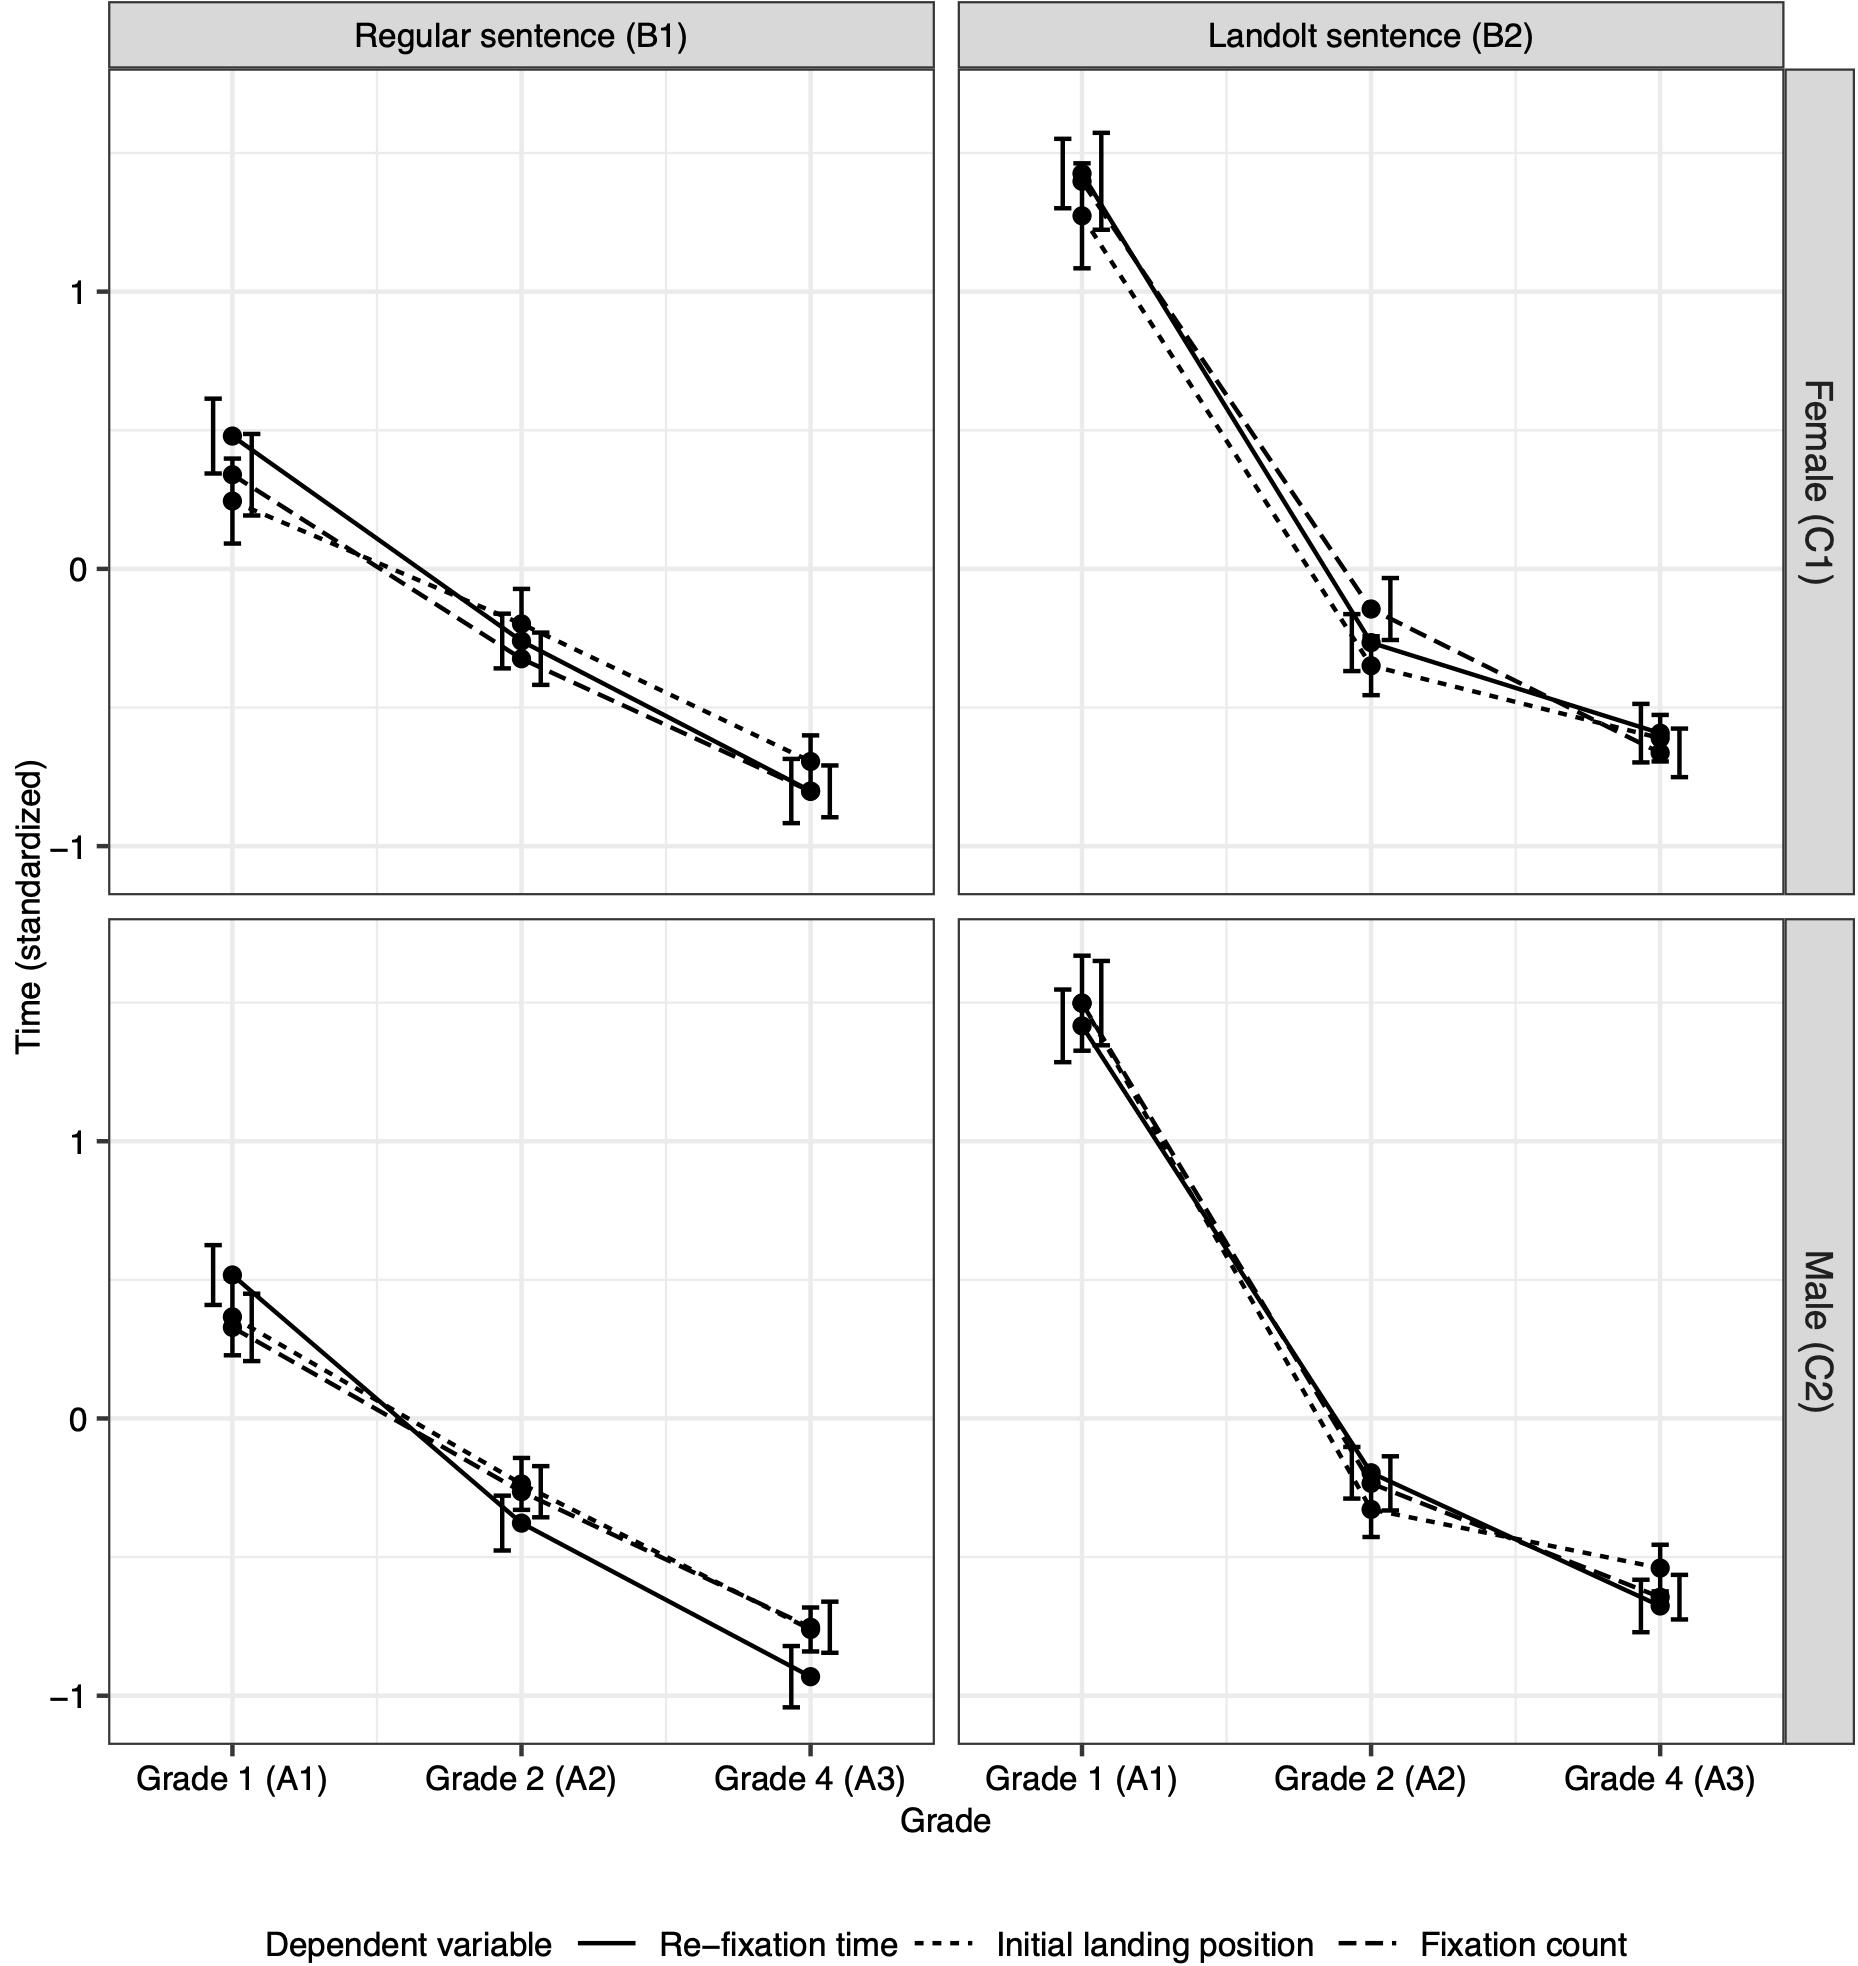
\includegraphics[width=1\linewidth]{semnova-man_files/figure-latex/variables-1} 

}

\caption{Re-fixation time (solid line), initial landing position (dotted line), and fixation count (dashed line) depending on sentence type (left panel: regular sentences; right panel: Landolt sentences), and sex (top panel: female; bottom panel: male) for the three measurement occasions (grade 1, grade 2, grade 4). The three variables were first averaged within children, then log-transformed and standardized. Shown are means across children. Error bars indicate standard errors.}\label{fig:variables}
\end{figure}

We will use the same contrast matrix for the within-subjects design as in the introduction \citep[see][Section 1.2 ``Latent Repeated Measures ANOVA'']{Langenberg2022z}. It is an orthogonal (i.e., linearly independent rows with length equal to one) polynomial contrast matrix and is given by:

\[
\mathbf{C} = \begin{pmatrix}
    0.408 & 0.408 & 0.408 & 0.408 & 0.408 & 0.408\\
    -0.5 & 0 & 0.5 & -0.5 & 0 & 0.5\\
    0.289 & -0.577 & 0.289 & 0.289 & -0.577 & 0.289\\
    -0.408 & -0.408 & -0.408 & 0.408 & 0.408 & 0.408\\
    0.5 & 0 & -0.5 & -0.5 & 0 & 0.5\\
    -0.289 & 0.577 & -0.289 & 0.289 & -0.577 & 0.289
\end{pmatrix}
\label{eq:introduction-c-matrix}
\]

In the following subsections, we will show numerous structural equation model (SEM) path diagrams that represent the estimated models. The entries from the inverse of the \(\mathbf{C}\) matrix (i.e.~the \(\mathbf{B}^{*}\) matrix) can be found on the regression arrows from the \(\boldsymbol{\pi}\) variables to the \(\boldsymbol{\eta}\) variables. It is noteworthy that the inverse of the \(\mathbf{C}\) matrix equals its transpose because it is an orthonormal matrix. This is a convenient property because the regression coefficients from the path diagrams can be found in both the \(\mathbf{B}^{*}\) and the (``rotated'\,') \(\mathbf{C}\) matrix. Thus, no inversion is needed to compare the path diagrams with the \(\mathbf{C}\) matrix.

\hypertarget{installation}{%
\chapter{Installation}\label{installation}}

This chapter will use Version~0.2.0 of the \emph{semnova} package. \emph{semnova} can be installed from \emph{CRAN}\footnote{\url{https://cran.r-project.org}}. However, we recommend to download the latest version from \emph{GitHub}\footnote{\url{https://github.com}}. The following lines of code can be used to install the package.

\begin{Shaded}
\begin{Highlighting}[]
\FunctionTok{install.packages}\NormalTok{(}\StringTok{"devtools"}\NormalTok{)}

\NormalTok{devtools}\SpecialCharTok{::}\FunctionTok{install\_github}\NormalTok{(}\StringTok{"langenberg/semnova@v0.2.0"}\NormalTok{)}

\FunctionTok{library}\NormalTok{(semnova)}
\end{Highlighting}
\end{Shaded}

Note that the \emph{devtools} package must be installed in order to be able to install software from \emph{GitHub}.

\hypertarget{within-subjects-designs}{%
\chapter{Within-Subjects Designs}\label{within-subjects-designs}}

For the first code example, we use the two within-subjects factors sentence type and grade from the motivating example with the manifest variable re-fixation time neglecting the between-subjects factor sex. The function \texttt{semnova()} offers a range of features and is used to estimate the first model:

\begin{Shaded}
\begin{Highlighting}[]
\NormalTok{fit }\OtherTok{\textless{}{-}} \FunctionTok{semnova}\NormalTok{(}
    \AttributeTok{data =}\NormalTok{ reading\_manifest,}
    \AttributeTok{id =} \StringTok{"id"}\NormalTok{, }
    \AttributeTok{dv =} \StringTok{"re\_fix\_time"}\NormalTok{,}
    \AttributeTok{within =} \FunctionTok{c}\NormalTok{(}\StringTok{"grade"}\NormalTok{, }\StringTok{"sentence"}\NormalTok{)}
\NormalTok{)}
\end{Highlighting}
\end{Shaded}

The function takes at least three arguments: \texttt{id} is a character vector of variables that uniquely identify the subjects, \texttt{dv} takes the name of the dependent variable, and \texttt{data} takes a data set in the long format (also called narrow format). Furthermore, \texttt{within} takes a vector of variables containing experimental within-subjects factors.

The next command is the \texttt{summary()} function which we use to extract the results from the model:

\begin{Shaded}
\begin{Highlighting}[]
\FunctionTok{summary}\NormalTok{(fit)}
\end{Highlighting}
\end{Shaded}

\begin{verbatim}
## Main and Interaction Effects:
##                  Chisq df Pr(>Chisq)    
## Intercept        4.711  1       0.03 *  
## grade          832.066  2     <2e-16 ***
## sentence       515.317  1     <2e-16 ***
## grade:sentence 234.919  2     <2e-16 ***
## ---
## Signif. codes:  0 '***' 0.001 '**' 0.01 '*' 0.05 '.' 0.1 ' ' 1
\end{verbatim}

The function prints hypothesis tests for each of the main and interaction effects. By default, the output contains a Wald test for the effects, future releases will include more statistics such as the likelihood ratio test and an approximate \(F\)-test. The factor grade has three levels and the test consequently has two degrees of freedom. All tests are highly significant, leading to the rejection of the null hypothesis and suggesting that the re-fixation time is neither constant across grade nor across the sentence types.

We can further use the \texttt{print()} function to print parameter estimates for each of the freely estimated model parameters. The following output is truncated after seven rows due to the large number of parameters.

\begin{Shaded}
\begin{Highlighting}[]
\FunctionTok{print}\NormalTok{(fit)}
\end{Highlighting}
\end{Shaded}

\begin{verbatim}
## 
## 
## parameter                    est          se      pvalue
## -------------------  -----------  ----------  ----------
## alpha_{pi,1,1}        -0.0677313   0.0312067   0.0299760
## sigma_{pi,1,1,1}^2     0.1636084   0.0178511   0.0000000
## sigma_{pi,1,2,1}^2    -0.0354949   0.0116314   0.0022760
## sigma_{pi,1,3,1}^2    -0.0165968   0.0082027   0.0430381
## sigma_{pi,1,4,1}^2    -0.0275617   0.0138830   0.0471122
## sigma_{pi,1,5,1}^2     0.0400701   0.0143246   0.0051533
## sigma_{pi,1,6,1}^2     0.0063447   0.0101050   0.5300847
## alpha_{pi,2,1}        -0.7971504   0.0279478   0.0000000
## sigma_{pi,2,2,1}^2     0.1312214   0.0143174   0.0000000
## sigma_{pi,2,3,1}^2    -0.0249054   0.0075061   0.0009066
## sigma_{pi,2,4,1}^2     0.0258745   0.0124476   0.0376466
## sigma_{pi,2,5,1}^2    -0.0147721   0.0125781   0.2402218
## sigma_{pi,2,6,1}^2     0.0255615   0.0092517   0.0057293
## alpha_{pi,3,1}         0.0681849   0.0200307   0.0006640
## sigma_{pi,3,3,1}^2     0.0674062   0.0073546   0.0000000
## sigma_{pi,3,4,1}^2     0.0096321   0.0088372   0.2757335
## sigma_{pi,3,5,1}^2     0.0341557   0.0093566   0.0002618
## sigma_{pi,3,6,1}^2     0.0085963   0.0065123   0.1868360
## alpha_{pi,4,1}        -0.7699475   0.0339175   0.0000000
## sigma_{pi,4,4,1}^2     0.1932668   0.0210871   0.0000000
## sigma_{pi,4,5,1}^2    -0.0326321   0.0154091   0.0341988
## sigma_{pi,4,6,1}^2    -0.0105359   0.0110000   0.3381557
## alpha_{pi,5,1}         0.5290506   0.0345798   0.0000000
## sigma_{pi,5,5,1}^2     0.2008881   0.0219187   0.0000000
## sigma_{pi,5,6,1}^2    -0.0264462   0.0113687   0.0200060
## alpha_{pi,6,1}        -0.0470649   0.0249530   0.0592762
## sigma_{pi,6,6,1}^2     0.1046057   0.0114134   0.0000000
\end{verbatim}

The \texttt{plot()} function further plots a path diagram for the model. shows two path diagrams. Per default, the diagram will only show regression arrows and measurement model arrows (see Figure~\ref{fig:within-manifest}). The \texttt{what} argument can be used to also draw intercepts, variances, covariances, residual variances and residual covariances (see Figure~\ref{fig:within-manifest-all}).

\begin{figure}

{\centering 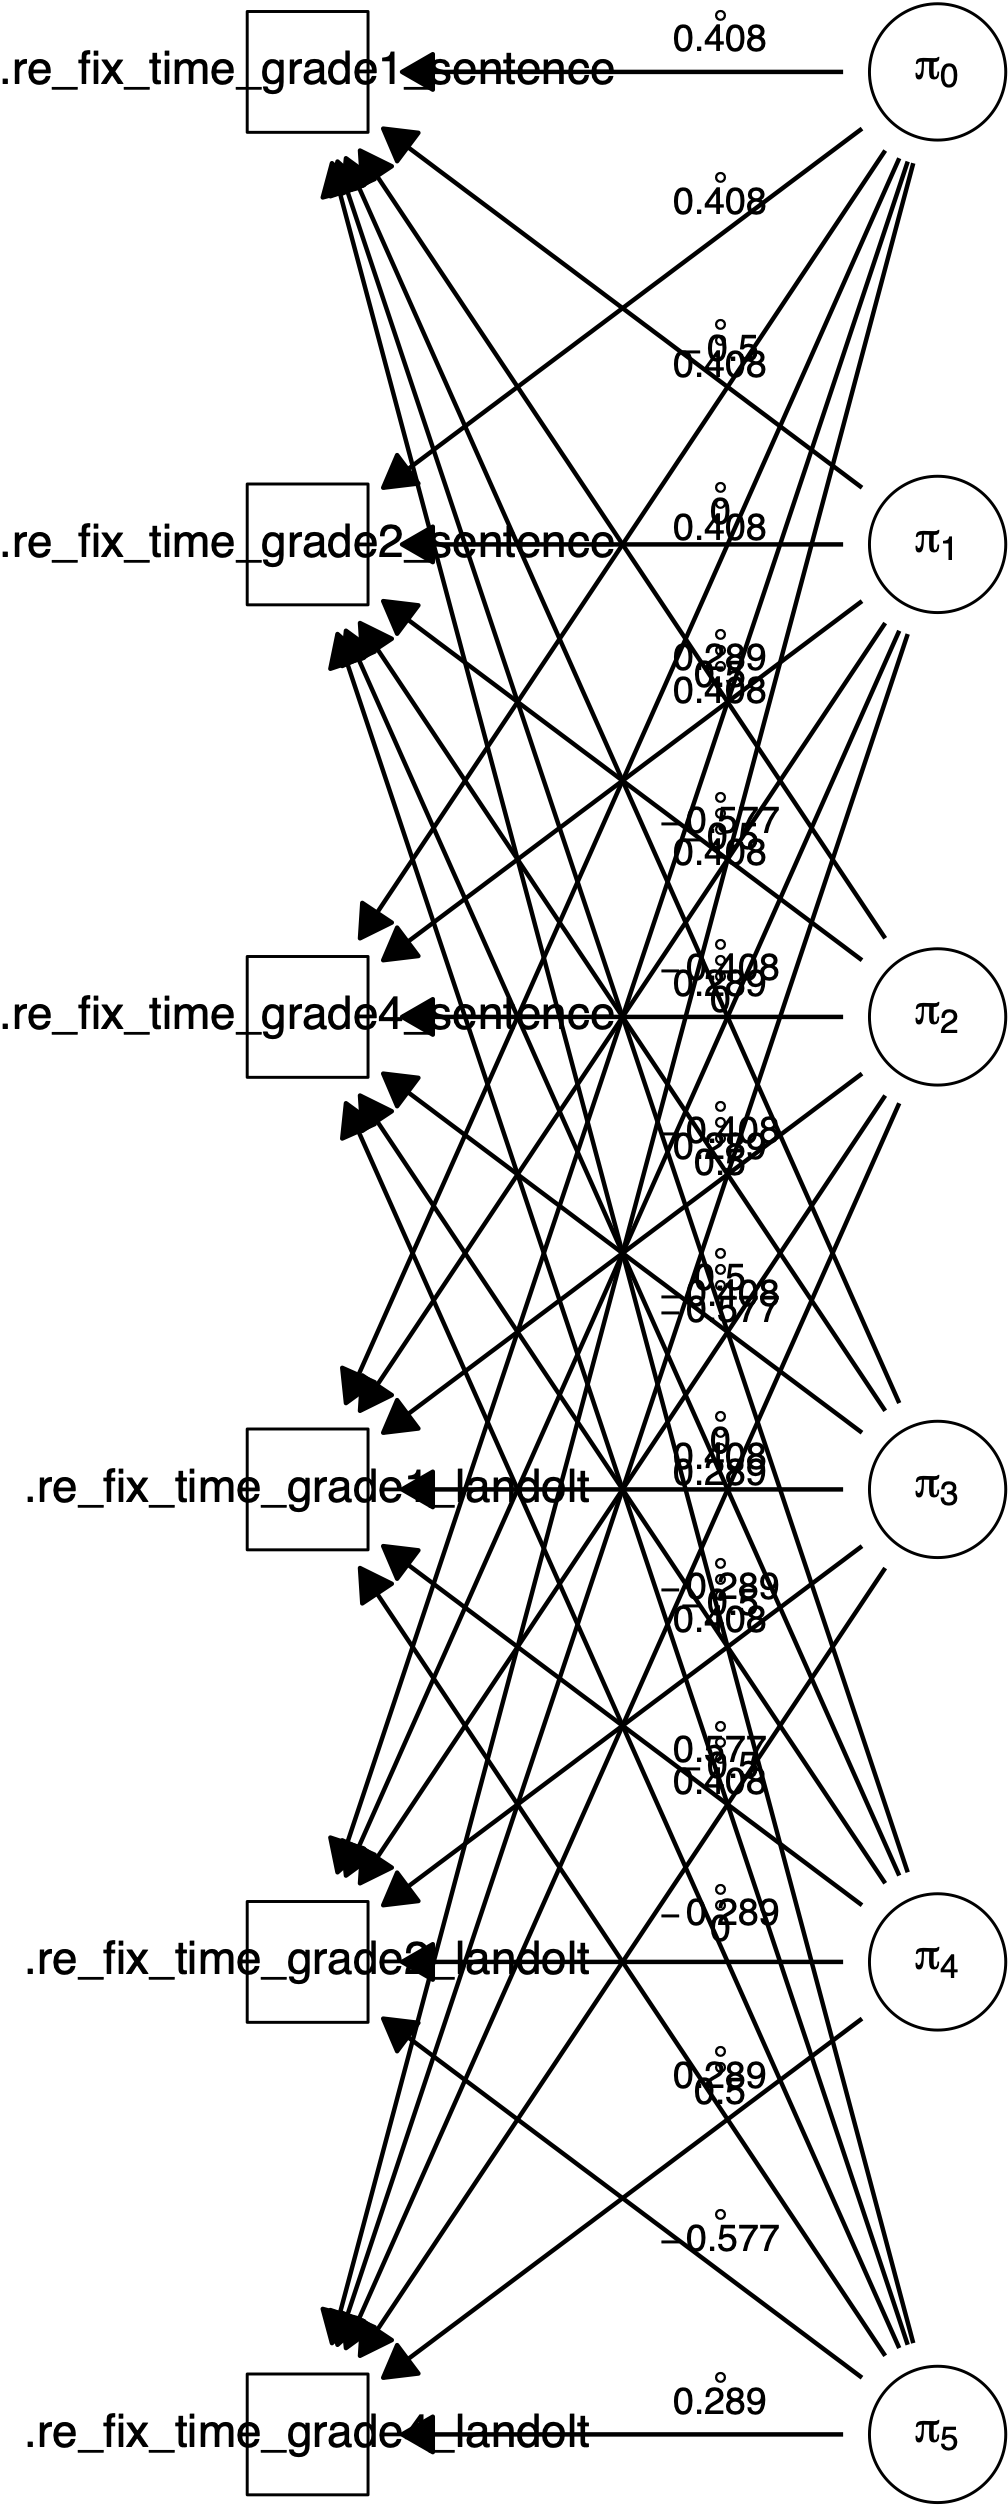
\includegraphics[width=0.35\linewidth]{semnova-man_files/figure-latex/within-manifest-1} 

}

\caption{Path diagram for a $2 \times 3$ (sentence $\times$ grade) within-subjects design with the manifest dependent variables re-fixation time. Created by \texttt{plot(fit)}.}\label{fig:within-manifest}
\end{figure}

\begin{figure}

{\centering 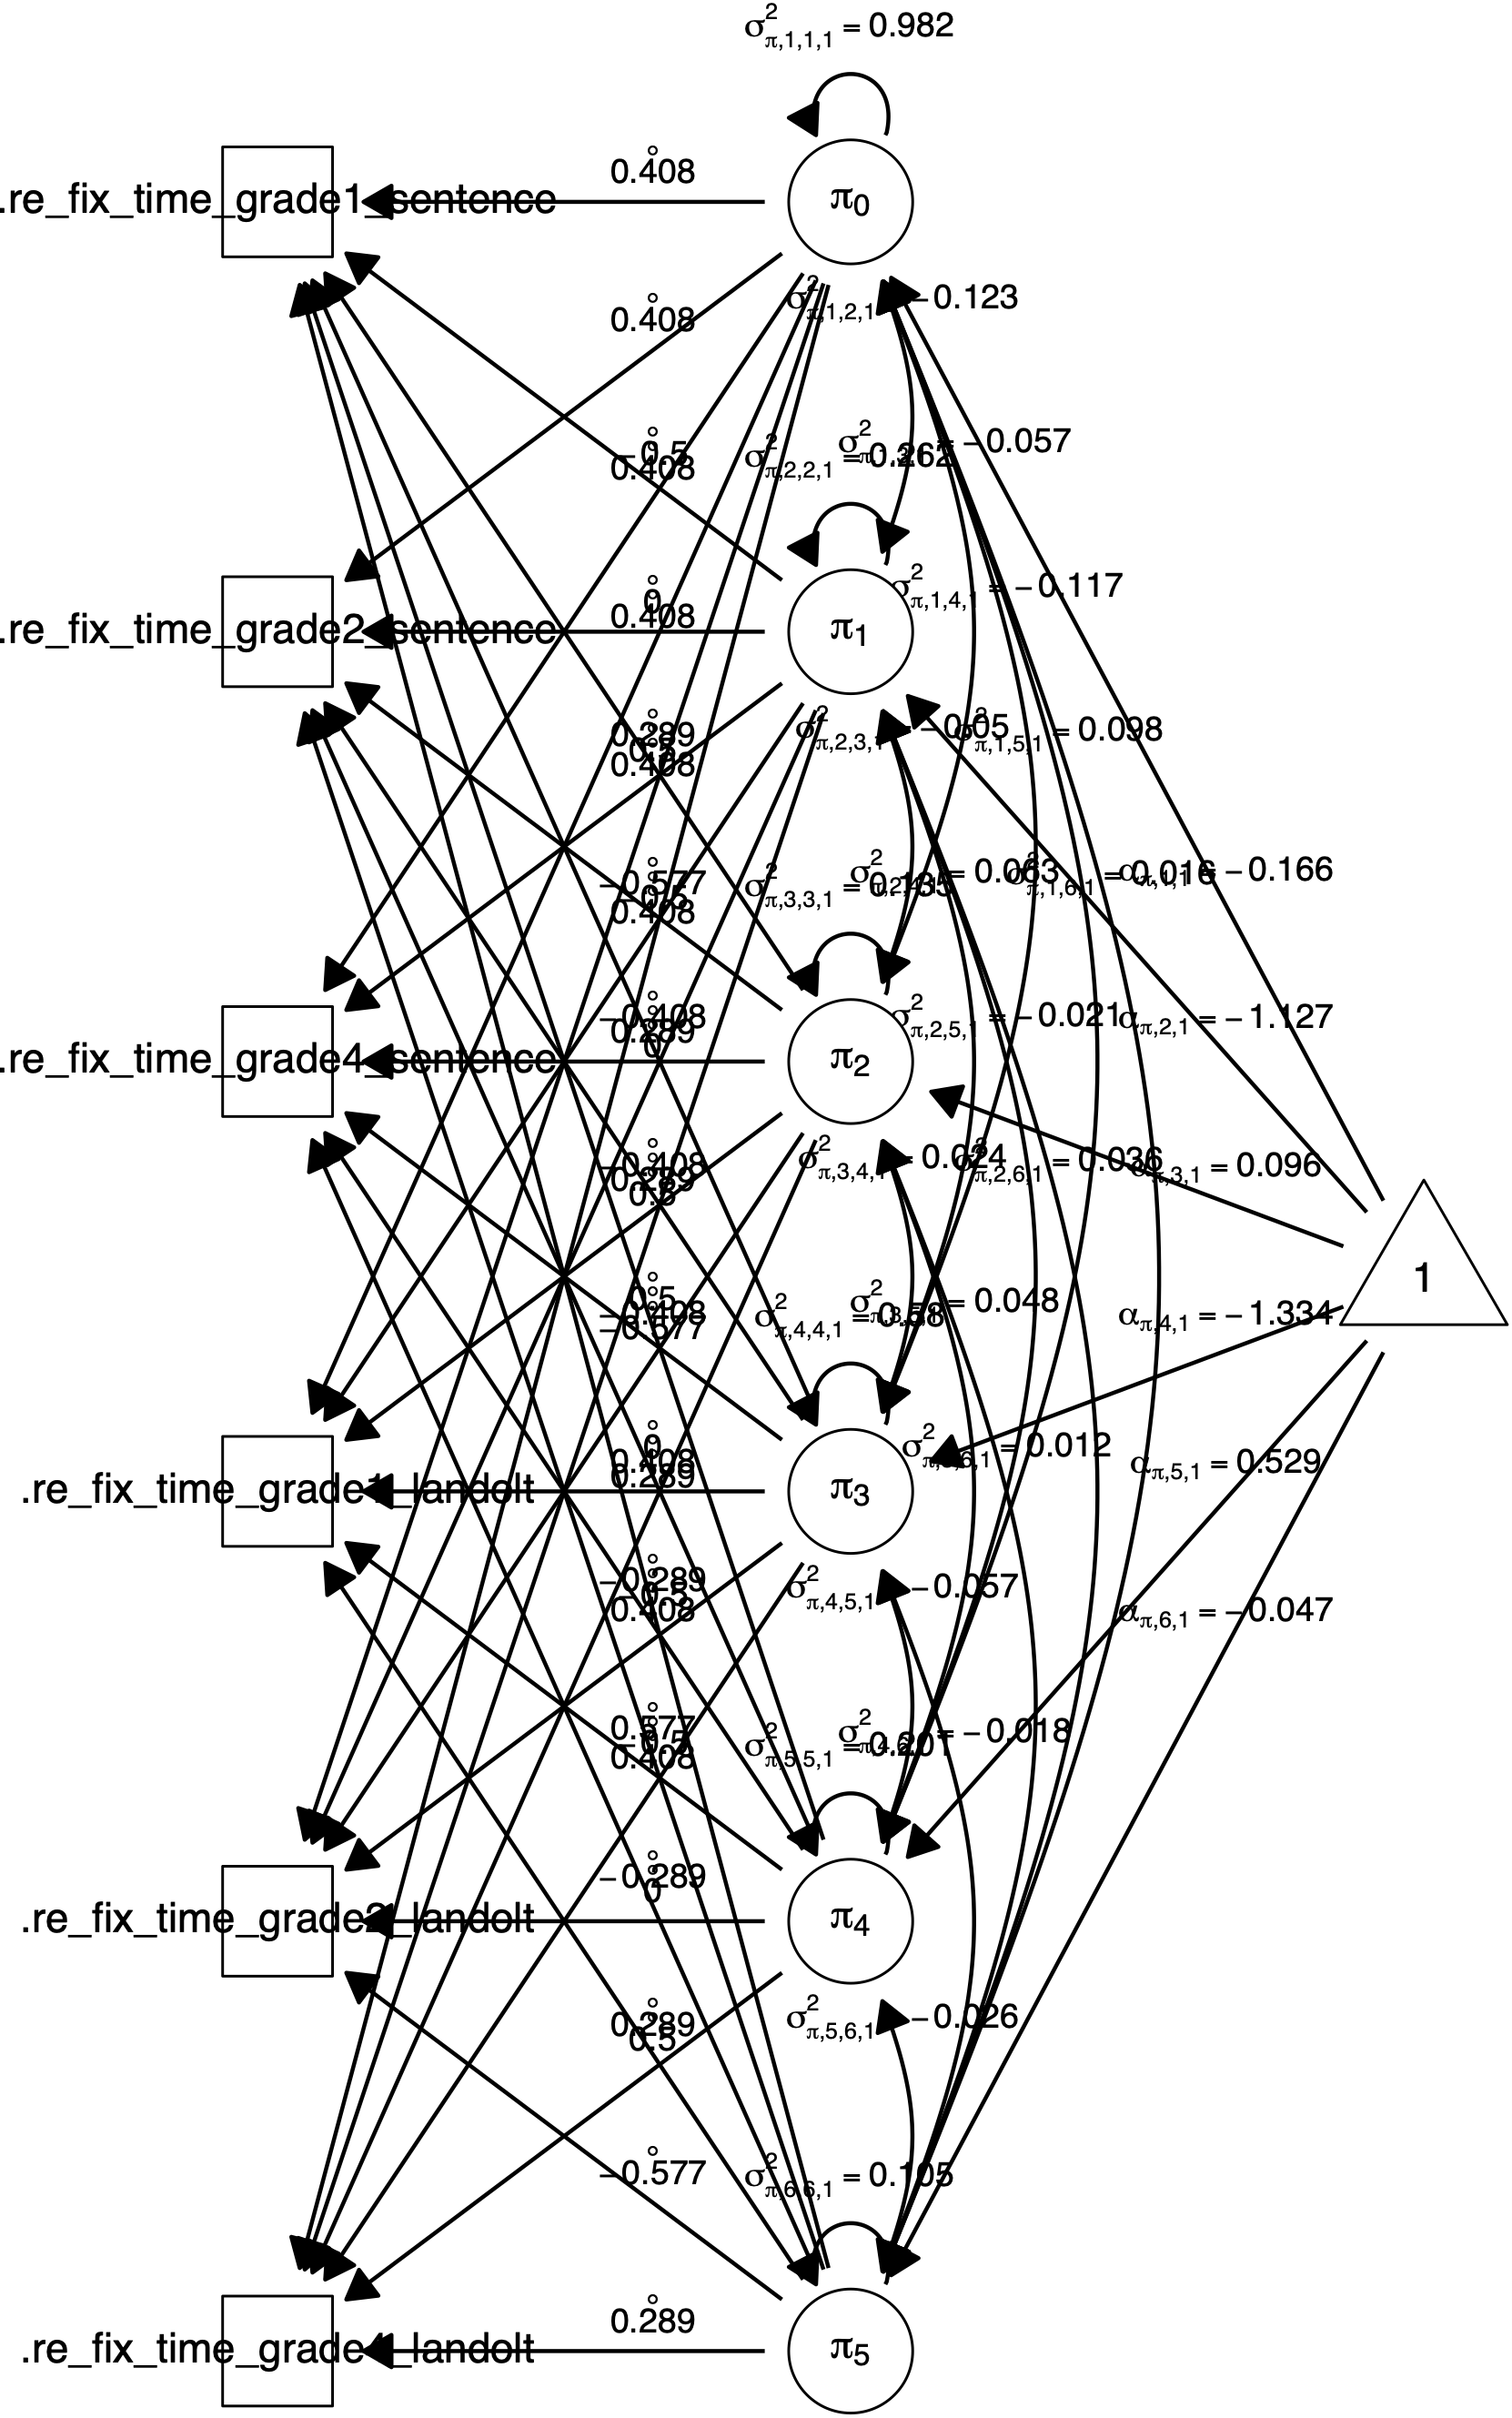
\includegraphics[width=0.57\linewidth]{semnova-man_files/figure-latex/within-manifest-all-1} 

}

\caption{Path diagram for a $2 \times 3$ (sentence $\times$ grade) within-subjects design with the manifest dependent variables re-fixation time. Created by \texttt{plot(fit, what = "all")}.}\label{fig:within-manifest-all}
\end{figure}

\hypertarget{sphericity}{%
\section{Sphericity}\label{sphericity}}

The next example shows how \emph{semnova} can be used to test for sphericity as described in Chapter 4 ``Understanding, Testing, and Relaxing Sphericity of Repeated Measures ANOVA with Manifest and Latent Variables Using SEM'' \citep{Langenberg2022z}. The \texttt{semnova()} function offers the \texttt{sphericity} argument to impose sphericity for a set of experimental factors. By default, the argument is \texttt{FALSE}. The argument can also take a list of vectors of experimental factors. Each vector describes an effect consisting of factor names (i.e., variable names) for which sphericity is to be assumed. For the factor grade, the code looks as follows:

\begin{verbatim}
## Chi-Squared Difference Test
## 
##               Df    AIC    BIC  Chisq Chisq diff Df diff Pr(>Chisq)    
## fit            0 1494.6 1579.0  0.000                                  
## fit_sph_grade  2 1521.1 1599.2 30.518     30.518       2  2.361e-07 ***
## ---
## Signif. codes:  0 '***' 0.001 '**' 0.01 '*' 0.05 '.' 0.1 ' ' 1
\end{verbatim}

All arguments are the same as for the previous example except for the \texttt{sphericity} argument. The factor grade has three levels and thus two effect variables. This command will force the variances of the effect variables \(\pi_1\) and \(\pi_2\) to be equal and their covariance to be zero. The \texttt{anova()} function can compare multiple models. Comparing a model with unconstrained covariance matrix to a model that imposes sphericity yields a formal test for sphericity.

The test is significant, suggesting that sphericity cannot be assumed. That is, either the variances of the effect variables are unequal, or the covariance is not zero. Thus, univariate test statistics cannot be used and multivariate tests should be preferred \citep[e.g.,][]{Lane2016a}. The test presents an alternative to the often-used Mauchly's sphericity test \citep{Mauchly1940a}.

The same test can be performed for the interaction of grade and sentence type because the effect consists of the two contrast variables \(\pi_4\) and \(\pi_5\) (i.e., the effect has two degrees of freedom):

\begin{Shaded}
\begin{Highlighting}[]
\NormalTok{fit\_sph\_grade\_sentence }\OtherTok{\textless{}{-}} \FunctionTok{semnova}\NormalTok{(}
    \AttributeTok{data =}\NormalTok{ reading\_manifest,}
    \AttributeTok{id =} \StringTok{"id"}\NormalTok{, }
    \AttributeTok{dv =} \StringTok{"re\_fix\_time"}\NormalTok{,}
    \AttributeTok{within =} \FunctionTok{c}\NormalTok{(}\StringTok{"grade"}\NormalTok{, }\StringTok{"sentence"}\NormalTok{),}
    \AttributeTok{sphericity =} \FunctionTok{list}\NormalTok{(}\FunctionTok{c}\NormalTok{(}\StringTok{"grade"}\NormalTok{, }\StringTok{"sentence"}\NormalTok{))}
\NormalTok{)}

\FunctionTok{anova}\NormalTok{(fit, fit\_sph\_grade\_sentence)}
\end{Highlighting}
\end{Shaded}

\begin{verbatim}
## Chi-Squared Difference Test
## 
##                        Df    AIC  BIC  Chisq Chisq diff Df diff Pr(>Chisq)    
## fit                     0 1494.6 1579  0.000                                  
## fit_sph_grade_sentence  2 1513.9 1592 23.262     23.262       2  8.884e-06 ***
## ---
## Signif. codes:  0 '***' 0.001 '**' 0.01 '*' 0.05 '.' 0.1 ' ' 1
\end{verbatim}

The \texttt{sphericity} argument is now a list consisting of a character vector with two elements indicating that sphericity is to be assumed for the interaction effect of grade and sentence type. The test is again significant and sphericity does not hold for the interaction effect.

Lastly, it is possible to perform an omnibus test for sphericity. This test assumes sphericity for all effects that have two or more degrees of freedom. Note that the variances and covariances of, and between, effect variables belonging to different effects (e.g., the contrast variable \(\pi_1\) from the main effect of grade and the contrast variable \(\pi_4\) from the interaction effect) are not constrained and are freely estimated. The following test will have four degrees of freedom (i.e., the sum of the degrees of freedom of the separate tests).

\begin{Shaded}
\begin{Highlighting}[]
\NormalTok{fit\_sph\_all }\OtherTok{\textless{}{-}} \FunctionTok{semnova}\NormalTok{(}
    \AttributeTok{data =}\NormalTok{ reading\_manifest,}
    \AttributeTok{id =} \StringTok{"id"}\NormalTok{, }
    \AttributeTok{dv =} \StringTok{"re\_fix\_time"}\NormalTok{,}
    \AttributeTok{within =} \FunctionTok{c}\NormalTok{(}\StringTok{"grade"}\NormalTok{, }\StringTok{"sentence"}\NormalTok{),}
    \AttributeTok{sphericity =} \FunctionTok{list}\NormalTok{(}\StringTok{"grade"}\NormalTok{, }\FunctionTok{c}\NormalTok{(}\StringTok{"grade"}\NormalTok{, }\StringTok{"sentence"}\NormalTok{))}
\NormalTok{)}

\FunctionTok{anova}\NormalTok{(fit, fit\_sph\_all)}
\end{Highlighting}
\end{Shaded}

\begin{verbatim}
## Chi-Squared Difference Test
## 
##             Df    AIC  BIC  Chisq Chisq diff Df diff Pr(>Chisq)    
## fit          0 1494.6 1579  0.000                                  
## fit_sph_all  4 1536.1 1608 49.511     49.511       4  4.567e-10 ***
## ---
## Signif. codes:  0 '***' 0.001 '**' 0.01 '*' 0.05 '.' 0.1 ' ' 1
\end{verbatim}

The test is also significant. We can use the test as an omnibus test to avoid multiple testing issues such as cumulative Type 1 errors. If the test is non-significant, we can assume sphericity for all effects and proceed with the more strict model which may give us a gain in statistical power \citep[e.g.,][]{Lane2016a, Muller1989a}. However, if the test is significant, we cannot say which of the effects violates the assumption and we have to perform both sphericity tests separately.

Note that, instead of \texttt{list(c("grade",\ "sentence"),\ "grade")}, the \texttt{sphericity} argument can also be set to \texttt{TRUE} imposing sphericity for all of the effects. The argument can also take a formula such as \texttt{FALSE\ \textasciitilde{}\ grade:sentence} which is equivalent to using \texttt{list(c("grade",\ "sentence"))}. The formula reads as ``do not assume sphericity (\texttt{FALSE}) except (\texttt{\textasciitilde{}}) for the interaction effect of sentence and grade (\texttt{sentence:grade})''.

\hypertarget{latent-variables}{%
\section{Latent Variables}\label{latent-variables}}

\hypertarget{measurement-model}{%
\subsection{Measurement Model}\label{measurement-model}}

The \texttt{semnova()} function can also incorporate latent variables. The input looks the same as for the very first example. Only this time, the \texttt{indicator} argument is provided, which takes the variable name of the data set that contains the names of the indicators. The variable named ``indicator'' from the example data set contains the values re\_fix\_dur, \texttt{"ini\_land\_pos"} and \texttt{"fix\_count"}. Furthermore, the argument \texttt{equal\_resid\_cov} can be used to allow for residual covariances between the indicators. Residual covariances between indicators are forced to be equal across experimental conditions. For instance, the covariances between the manifest variables of re-fixation time will be the same across all of the six experimental conditions. In this example, we use the variables re-fixation time, initial landing position and fixation count to form a latent variable that measures reading ability. By default, \emph{semnova} uses a congeneric measurement model with strong measurement invariance and the effect-code identification scheme \citep{Little2006a} to set the scale for the latent variables \citep[see also][Section 2.4.1 ``Defining the Model'']{Langenberg2022z}. We will further use full information maximum likelihood for this example because of several missing values by using \texttt{missing\ =\ "fiml"}. Full information maximum likelihood is implemented in the \emph{lavaan} package and the argument is passed on to \emph{lavaan}.

\begin{Shaded}
\begin{Highlighting}[]
\NormalTok{fit\_latent }\OtherTok{\textless{}{-}} \FunctionTok{semnova}\NormalTok{(}
    \AttributeTok{data =}\NormalTok{ reading\_latent,}
    \AttributeTok{id =} \StringTok{"id"}\NormalTok{, }
    \AttributeTok{dv =} \StringTok{"dv"}\NormalTok{,}
    \AttributeTok{indicator =} \StringTok{"indicator"}\NormalTok{,}
    \AttributeTok{equal\_resid\_cov =} \FunctionTok{list}\NormalTok{(}\StringTok{"ini\_land\_pos"}\NormalTok{, }\StringTok{"fix\_count"}\NormalTok{),}
    \AttributeTok{within =} \FunctionTok{c}\NormalTok{(}\StringTok{"grade"}\NormalTok{, }\StringTok{"sentence"}\NormalTok{),}
    \AttributeTok{missing =} \StringTok{"fiml"}
\NormalTok{)}

\FunctionTok{summary}\NormalTok{(fit\_latent)}
\end{Highlighting}
\end{Shaded}

\begin{verbatim}
## Fit measures:
## 
## Chisq(138) = 461.551, p = 0
## CFI = 0.861
## TLI = 0.845
## RMSEA = 0.094 [0.084, 0.103]
## 
## ##############################
## 
## Main and Interaction Effects:
##                   Chisq df Pr(>Chisq)    
## Intercept         0.416  1      0.519    
## grade          1432.334  2     <2e-16 ***
## sentence       1037.801  1     <2e-16 ***
## grade:sentence  607.323  2     <2e-16 ***
## ---
## Signif. codes:  0 '***' 0.001 '**' 0.01 '*' 0.05 '.' 0.1 ' ' 1
\end{verbatim}

The output now contains a section for fit indices in addition to hypothesis tests. The hypothesis tests are again significant. The fit is not very good but the example is intended to demonstrate the basic usage of the software package. The fit can be poor for several reasons. For instance, measurement invariance across the experimental conditions may not hold. This assumption will be examined in the next section. As a consequence, we should be very cautious when interpreting parameter estimates and hypothesis tests.

In complex latent variables models, negative (residual) variances are also an issue. This can happen if the variances of the latent variables are very small as compared to residual variances (i.e., very low reliability of manifest variables) of the manifest variables or vice versa (i.e., manifest variables are highly correlated). The \texttt{reliabilities()} function serves as a diagnostic tool and prints the reliabilities and variances of both the manifest and latent variables:

\begin{Shaded}
\begin{Highlighting}[]
\FunctionTok{reliabilities}\NormalTok{(fit\_latent)}
\end{Highlighting}
\end{Shaded}

\begin{verbatim}
## indicator      sentence   grade       reliability   sigma_eta      lambda       eps_y
## -------------  ---------  ---------  ------------  ----------  ----------  ----------
## fix_count      grade1     sentence      0.6363140   0.4724375   0.9959292   0.2678282
## ini_land_pos   grade1     sentence      0.4610548   0.4724375   0.9304984   0.4781539
## re_fix_time    grade1     sentence      0.6672992   0.4724375   1.0735725   0.2714815
## fix_count      grade2     sentence      0.7140289   0.3885014   0.9959292   0.1543319
## ini_land_pos   grade2     sentence      0.5883054   0.3885014   0.9304984   0.2353945
## re_fix_time    grade2     sentence      0.9671821   0.3885014   1.0735725   0.0151935
## fix_count      grade4     sentence      0.5436482   0.1850009   0.9959292   0.1540326
## ini_land_pos   grade4     sentence      0.4849815   0.1850009   0.9304984   0.1700994
## re_fix_time    grade4     sentence      0.8347808   0.1850009   1.0735725   0.0422012
## fix_count      grade1     landolt       0.5371139   0.1755438   0.9959292   0.1500550
## ini_land_pos   grade1     landolt       0.4112846   0.1755438   0.9304984   0.2175604
## re_fix_time    grade1     landolt       0.6084315   0.1755438   1.0735725   0.1302100
## fix_count      grade2     landolt       0.4555433   0.1123143   0.9959292   0.1331452
## ini_land_pos   grade2     landolt       0.3650680   0.1123143   0.9304984   0.1691296
## re_fix_time    grade2     landolt       0.4975977   0.1123143   1.0735725   0.1306986
## fix_count      grade4     landolt       0.3834018   0.0987020   0.9959292   0.1574457
## ini_land_pos   grade4     landolt       0.3831102   0.0987020   0.9304984   0.1376071
## re_fix_time    grade4     landolt       0.3894837   0.0987020   1.0735725   0.1783186
\end{verbatim}

``sigma\_eta'' contains the model implied variances of the latent dependent variables \(\boldsymbol{\eta}\) (i.e., the variances are fixed to zero in laten repeated measures ANOVA {[}L-RM-ANOVA{]} and can be calculated from the variances of the \(\boldsymbol{\pi}\) variables). ``lambda'' contains the factor loadings of the manifest variables on the latent variables. ``eps\_y'' contains the residual variances of the manifest variables. We see that none of the residual variances is negative. The smallest reliability is .37 which is rather low. In contrast, the highest reliability is .97 which is very high. The analysis serves as an example and we will not further examine the reliabilities and residual variances. In practice, however, we should further investigate possible reasons for the poor fit.

Figure~\ref{fig:within-latent} shows a path diagram of the model including all of the parameters.

\begin{figure}

{\centering 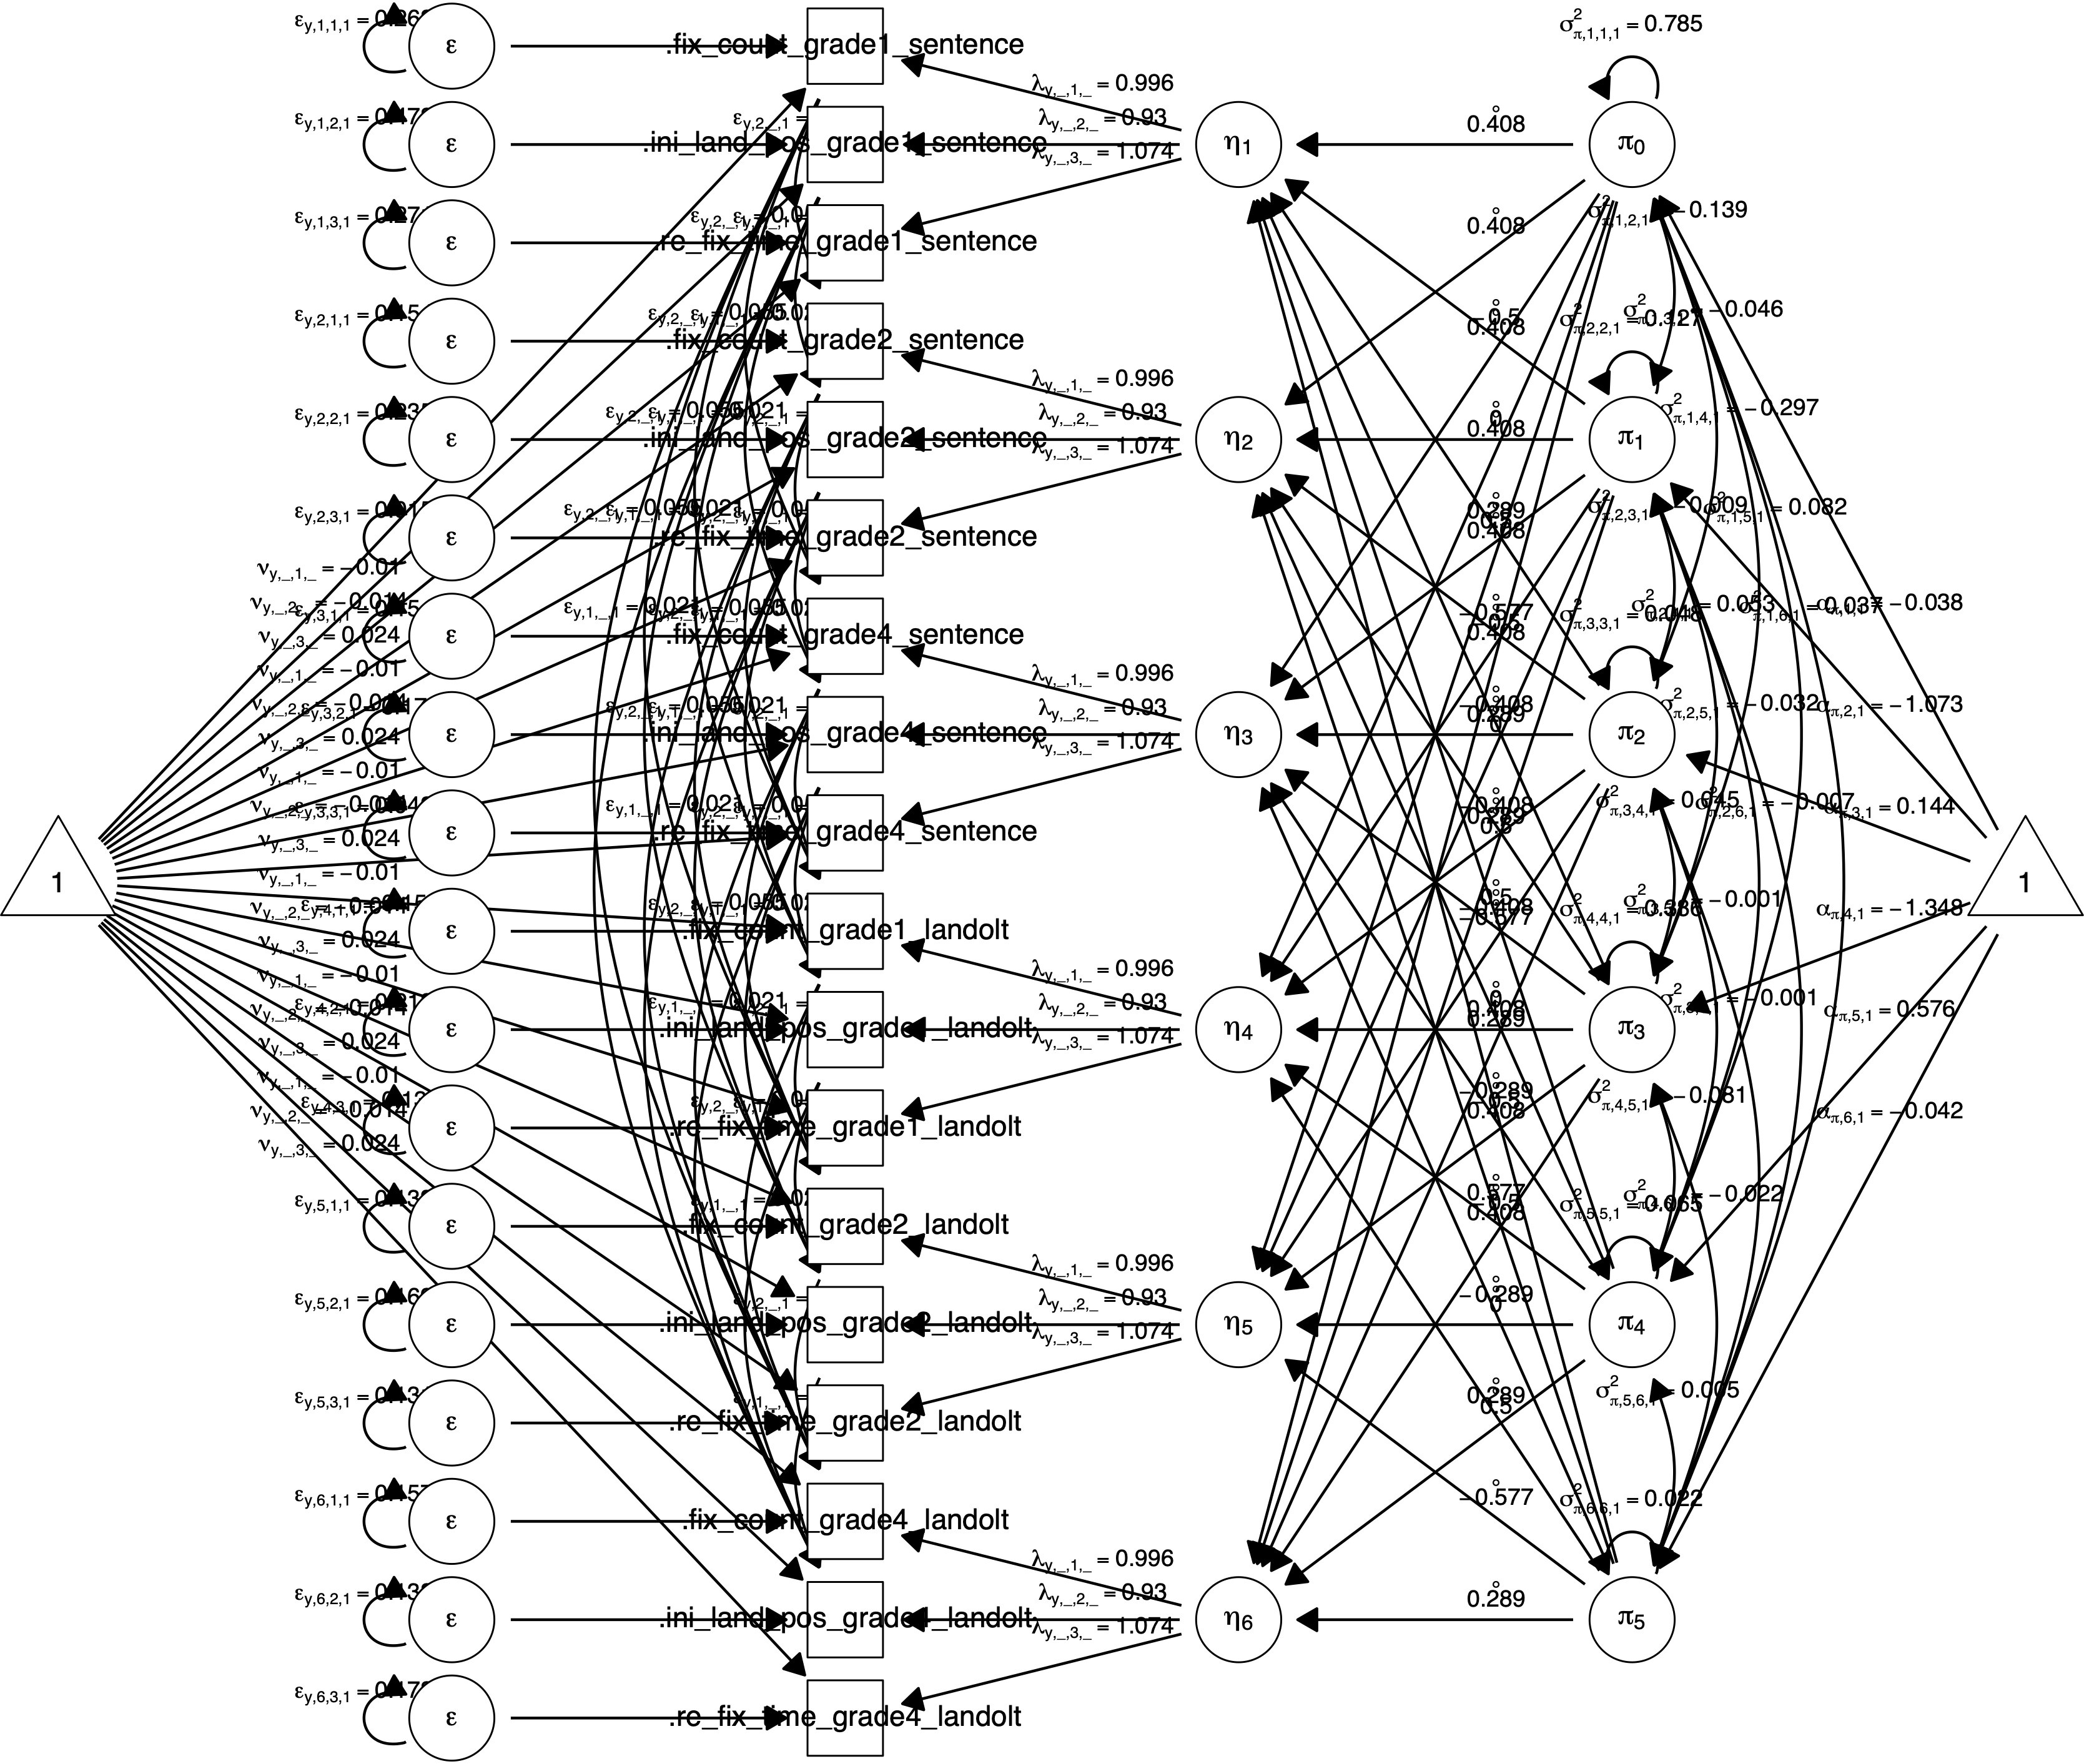
\includegraphics[width=1\linewidth]{semnova-man_files/figure-latex/within-latent-1} 

}

\caption{Path diagram created by \texttt{plot(fit\_latent, what = "all")} for a $2 \times 3$ (sentence $\times$ grade) within-subjects design with the latent dependent variable reading ability measured by the three manifest variables re-fixation time, initial landing position and fixation count.}\label{fig:within-latent}
\end{figure}

\hypertarget{measurement-invariance}{%
\subsection{Measurement Invariance}\label{measurement-invariance}}

Measurement invariance is an important assumption when using latent variables. This assumption is oftentimes implicitly assumed when using traditional repeated measures (RM-ANOVA). RM-ANOVA cannot handle latent variables and indicators are averaged to manifest composite or sum scores in order to be able to use RM-ANOVA. This approach implicitly assumes a parallel measurement model across the six experimental conditions but the assumption is not explicitly tested. In order to be able to compare the means of latent variables, we need strong measurement invariance \citep[see][Section 2.4 ``Latent Repeated Measures ANOVA (L-RM-ANOVA)'']{Langenberg2022z}, that is, equal loadings and equal intercepts across the experimental conditions. With \emph{semnova}, we can actually test for measurement invariance. As described in the previous example, \emph{semnova} uses a congeneric measurement model. The \texttt{invariance\_within} argument can be set to either of \texttt{"configural"} (equal model structure), \texttt{"weak"} (equal loadings), \texttt{"strong"} (equal loadings and intercepts), or \texttt{"strict"} (equal loadings, intercepts and residual variances):

\begin{Shaded}
\begin{Highlighting}[]
\NormalTok{fit\_latent\_configMI }\OtherTok{\textless{}{-}} \FunctionTok{semnova}\NormalTok{(}
    \AttributeTok{data =}\NormalTok{ reading\_latent,}
    \AttributeTok{id =} \StringTok{"id"}\NormalTok{, }
    \AttributeTok{dv =} \StringTok{"dv"}\NormalTok{,}
    \AttributeTok{indicator =} \StringTok{"indicator"}\NormalTok{,}
    \AttributeTok{equal\_resid\_cov =} \FunctionTok{list}\NormalTok{(}\StringTok{"ini\_land\_pos"}\NormalTok{, }\StringTok{"fix\_count"}\NormalTok{),}
    \AttributeTok{within =} \FunctionTok{c}\NormalTok{(}\StringTok{"grade"}\NormalTok{, }\StringTok{"sentence"}\NormalTok{),}
    \AttributeTok{missing =} \StringTok{"fiml"}\NormalTok{,}
    \AttributeTok{invariance\_within =} \StringTok{"configural"}
\NormalTok{)}

\NormalTok{fit\_latent\_weakMI }\OtherTok{\textless{}{-}} \FunctionTok{semnova}\NormalTok{(}
    \AttributeTok{data =}\NormalTok{ reading\_latent,}
    \AttributeTok{id =} \StringTok{"id"}\NormalTok{, }
    \AttributeTok{dv =} \StringTok{"dv"}\NormalTok{,}
    \AttributeTok{indicator =} \StringTok{"indicator"}\NormalTok{,}
    \AttributeTok{equal\_resid\_cov =} \FunctionTok{list}\NormalTok{(}\StringTok{"ini\_land\_pos"}\NormalTok{, }\StringTok{"fix\_count"}\NormalTok{),}
    \AttributeTok{within =} \FunctionTok{c}\NormalTok{(}\StringTok{"grade"}\NormalTok{, }\StringTok{"sentence"}\NormalTok{),}
    \AttributeTok{missing =} \StringTok{"fiml"}\NormalTok{,}
    \AttributeTok{invariance\_within =} \StringTok{"weak"}
\NormalTok{)}

\NormalTok{fit\_latent\_strongMI }\OtherTok{\textless{}{-}} \FunctionTok{semnova}\NormalTok{(}
    \AttributeTok{data =}\NormalTok{ reading\_latent,}
    \AttributeTok{id =} \StringTok{"id"}\NormalTok{, }
    \AttributeTok{dv =} \StringTok{"dv"}\NormalTok{,}
    \AttributeTok{indicator =} \StringTok{"indicator"}\NormalTok{,}
    \AttributeTok{equal\_resid\_cov =} \FunctionTok{list}\NormalTok{(}\StringTok{"ini\_land\_pos"}\NormalTok{, }\StringTok{"fix\_count"}\NormalTok{),}
    \AttributeTok{within =} \FunctionTok{c}\NormalTok{(}\StringTok{"grade"}\NormalTok{, }\StringTok{"sentence"}\NormalTok{),}
    \AttributeTok{missing =} \StringTok{"fiml"}\NormalTok{,}
    \AttributeTok{invariance\_within =} \StringTok{"strong"}
\NormalTok{)}

\NormalTok{fit\_latent\_strictMI }\OtherTok{\textless{}{-}} \FunctionTok{semnova}\NormalTok{(}
    \AttributeTok{data =}\NormalTok{ reading\_latent,}
    \AttributeTok{id =} \StringTok{"id"}\NormalTok{, }
    \AttributeTok{dv =} \StringTok{"dv"}\NormalTok{,}
    \AttributeTok{indicator =} \StringTok{"indicator"}\NormalTok{,}
    \AttributeTok{equal\_resid\_cov =} \FunctionTok{list}\NormalTok{(}\StringTok{"ini\_land\_pos"}\NormalTok{, }\StringTok{"fix\_count"}\NormalTok{),}
    \AttributeTok{within =} \FunctionTok{c}\NormalTok{(}\StringTok{"grade"}\NormalTok{, }\StringTok{"sentence"}\NormalTok{),}
    \AttributeTok{missing =} \StringTok{"fiml"}\NormalTok{,}
    \AttributeTok{invariance\_within =} \StringTok{"strict"}
\NormalTok{)}

\FunctionTok{anova}\NormalTok{(}
\NormalTok{    fit\_latent\_configMI, }
\NormalTok{    fit\_latent\_weakMI, }
\NormalTok{    fit\_latent\_strongMI, }
\NormalTok{    fit\_latent\_strictMI}
\NormalTok{)}
\end{Highlighting}
\end{Shaded}

\begin{verbatim}
## Chi-Squared Difference Test
## 
##                      Df    AIC    BIC  Chisq Chisq diff Df diff Pr(>Chisq)    
## fit_latent_configMI 118 5467.5 5722.2 248.11                                  
## fit_latent_weakMI   128 5579.8 5798.6 380.44    132.332      10  < 2.2e-16 ***
## fit_latent_strongMI 138 5640.9 5823.9 461.55     81.114      10  3.036e-13 ***
## fit_latent_strictMI 153 5875.1 6004.2 725.68    264.131      15  < 2.2e-16 ***
## ---
## Signif. codes:  0 '***' 0.001 '**' 0.01 '*' 0.05 '.' 0.1 ' ' 1
\end{verbatim}

Using the \texttt{anova()} function, we can compare the four models. All tests are highly significant indicating that they do not fit equally well. Thus, we cannot assume any degree of measurement invariance. As a consequence, we should be very cautious when interpreting parameter estimates and hypothesis tests.

\hypertarget{between-subjects-designs}{%
\chapter{Between-Subjects Designs}\label{between-subjects-designs}}

The \texttt{semnova()} function can also be used with between-subjects factors and covariates. The \texttt{between} argument takes a vector of between-subjects factors (i.e., grouping variables). We estimate the same manifest model as in the very first example with the additional between-subjects factor sex. Using the \texttt{between} argument will cause \emph{semnova} to estimate a multi-group model:

\begin{Shaded}
\begin{Highlighting}[]
\NormalTok{fit\_btw }\OtherTok{\textless{}{-}} \FunctionTok{semnova}\NormalTok{(}
    \AttributeTok{data =}\NormalTok{ reading\_manifest,}
    \AttributeTok{id =} \StringTok{"id"}\NormalTok{, }
    \AttributeTok{dv =} \StringTok{"re\_fix\_time"}\NormalTok{,}
    \AttributeTok{within =} \FunctionTok{c}\NormalTok{(}\StringTok{"grade"}\NormalTok{, }\StringTok{"sentence"}\NormalTok{),}
    \AttributeTok{between =} \StringTok{"sex"}
\NormalTok{)}

\FunctionTok{summary}\NormalTok{(fit\_btw)}
\end{Highlighting}
\end{Shaded}

\begin{verbatim}
## Main and Interaction Effects:
##                      Chisq df Pr(>Chisq)    
## Intercept            1.505  1      0.220    
## grade              354.755  2     <2e-16 ***
## sentence           381.882  1     <2e-16 ***
## grade:sentence      84.370  2     <2e-16 ***
## sex                  0.192  1      0.661    
## grade:sex            1.969  2      0.374    
## sentence:sex         1.800  1      0.180    
## grade:sentence:sex   1.959  2      0.376    
## ---
## Signif. codes:  0 '***' 0.001 '**' 0.01 '*' 0.05 '.' 0.1 ' ' 1
\end{verbatim}

When including between-subjects effects, hypothesis tests correspond to Type III sums of squares in ANOVA. Type III sums of squares do not take unbalanced group sizes into account as apposed to average effects \citep[e.g.,][]{Graefe2020a}. Tests for average effects remain work in progress and may be included in future releases.

Main and interaction effects for the within-subjects factors are again significant. Main and interaction effects involving the between-subjects factor sex are non-significant indicating that no differences exist across genders.

\begin{figure}

{\centering 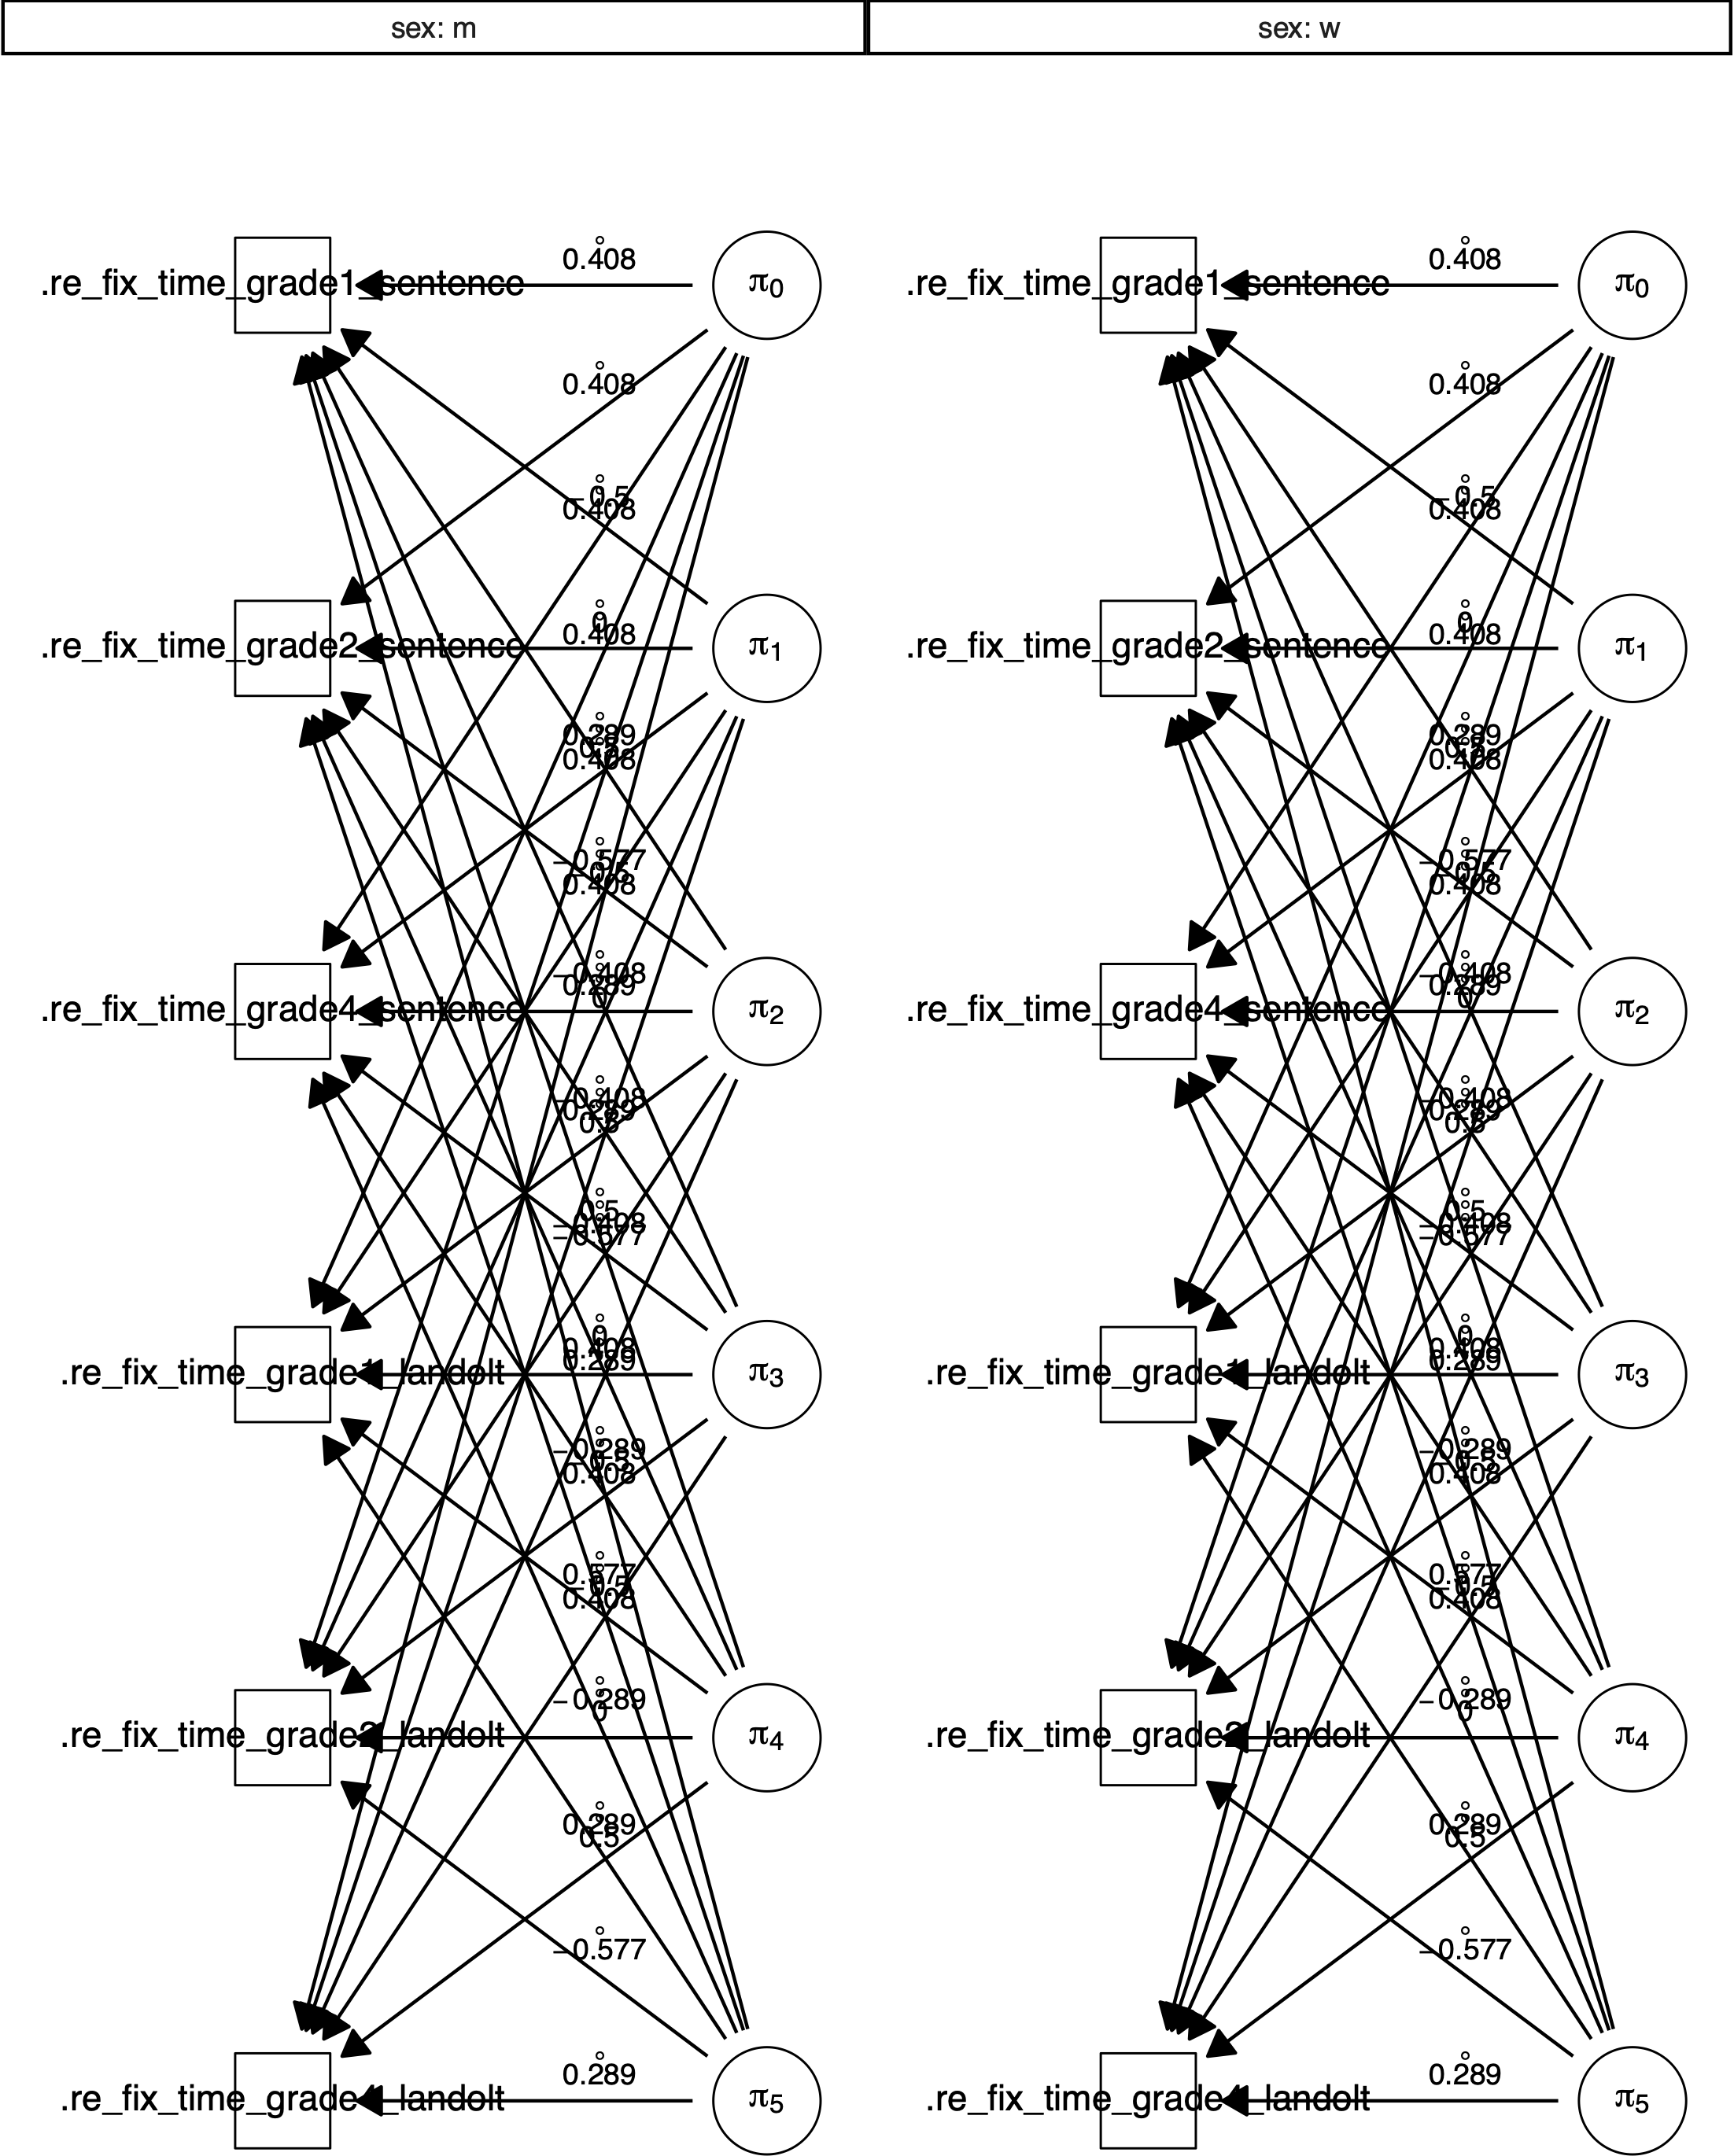
\includegraphics[width=1\linewidth]{semnova-man_files/figure-latex/software-between-manifest-1} 

}

\caption{Path diagram created by \texttt{plot(fit\_btw)} for a $2 \times 3 \times 2$ (sentence $\times$ grade $\times$ sex) mixed design design with the manifest dependent variable re-fixation time.}\label{fig:software-between-manifest}
\end{figure}

\hypertarget{latent-variables-1}{%
\section{Latent Variables}\label{latent-variables-1}}

\hypertarget{measurement-model-1}{%
\subsection{Measurement Model}\label{measurement-model-1}}

The multi-group approach can also be used with latent variables. The command is identical to the previous purely within-subjects example that includes latent variables, except for the additional \texttt{between} argument.

\begin{Shaded}
\begin{Highlighting}[]
\NormalTok{fit\_btw\_latent }\OtherTok{\textless{}{-}} \FunctionTok{semnova}\NormalTok{(}
    \AttributeTok{data =}\NormalTok{ reading\_latent,}
    \AttributeTok{id =} \StringTok{"id"}\NormalTok{, }
    \AttributeTok{dv =} \StringTok{"dv"}\NormalTok{,}
    \AttributeTok{indicator =} \StringTok{"indicator"}\NormalTok{,}
    \AttributeTok{equal\_resid\_cov =} \FunctionTok{list}\NormalTok{(}\StringTok{"ini\_land\_pos"}\NormalTok{, }\StringTok{"fix\_count"}\NormalTok{),}
    \AttributeTok{between =} \StringTok{"sex"}\NormalTok{,}
    \AttributeTok{within =} \FunctionTok{c}\NormalTok{(}\StringTok{"grade"}\NormalTok{, }\StringTok{"sentence"}\NormalTok{),}
    \AttributeTok{missing =} \StringTok{"fiml"}
\NormalTok{)}

\FunctionTok{summary}\NormalTok{(fit\_btw\_latent)}
\end{Highlighting}
\end{Shaded}

\begin{verbatim}
## Fit measures:
## 
## Chisq(280) = 693.254, p = 0
## CFI = 0.833
## TLI = 0.817
## RMSEA = 0.105 [0.095, 0.115]
## 
## ##############################
## 
## Main and Interaction Effects:
##                      Chisq df Pr(>Chisq)    
## Intercept            0.035  1      0.852    
## grade              765.984  2     <2e-16 ***
## sentence           651.753  1     <2e-16 ***
## grade:sentence     310.771  2     <2e-16 ***
## sex                  0.253  1      0.615    
## grade:sex            1.446  2      0.485    
## sentence:sex         1.469  1      0.226    
## grade:sentence:sex   1.993  2      0.369    
## ---
## Signif. codes:  0 '***' 0.001 '**' 0.01 '*' 0.05 '.' 0.1 ' ' 1
\end{verbatim}

The model fit is again not very good. Hypothesis tests show the same pattern as for the model using only the manifest variable re-fixation time. A path diagram of the model is shown in Figure~\ref{fig:software-between-latent}.

\begin{figure}

{\centering 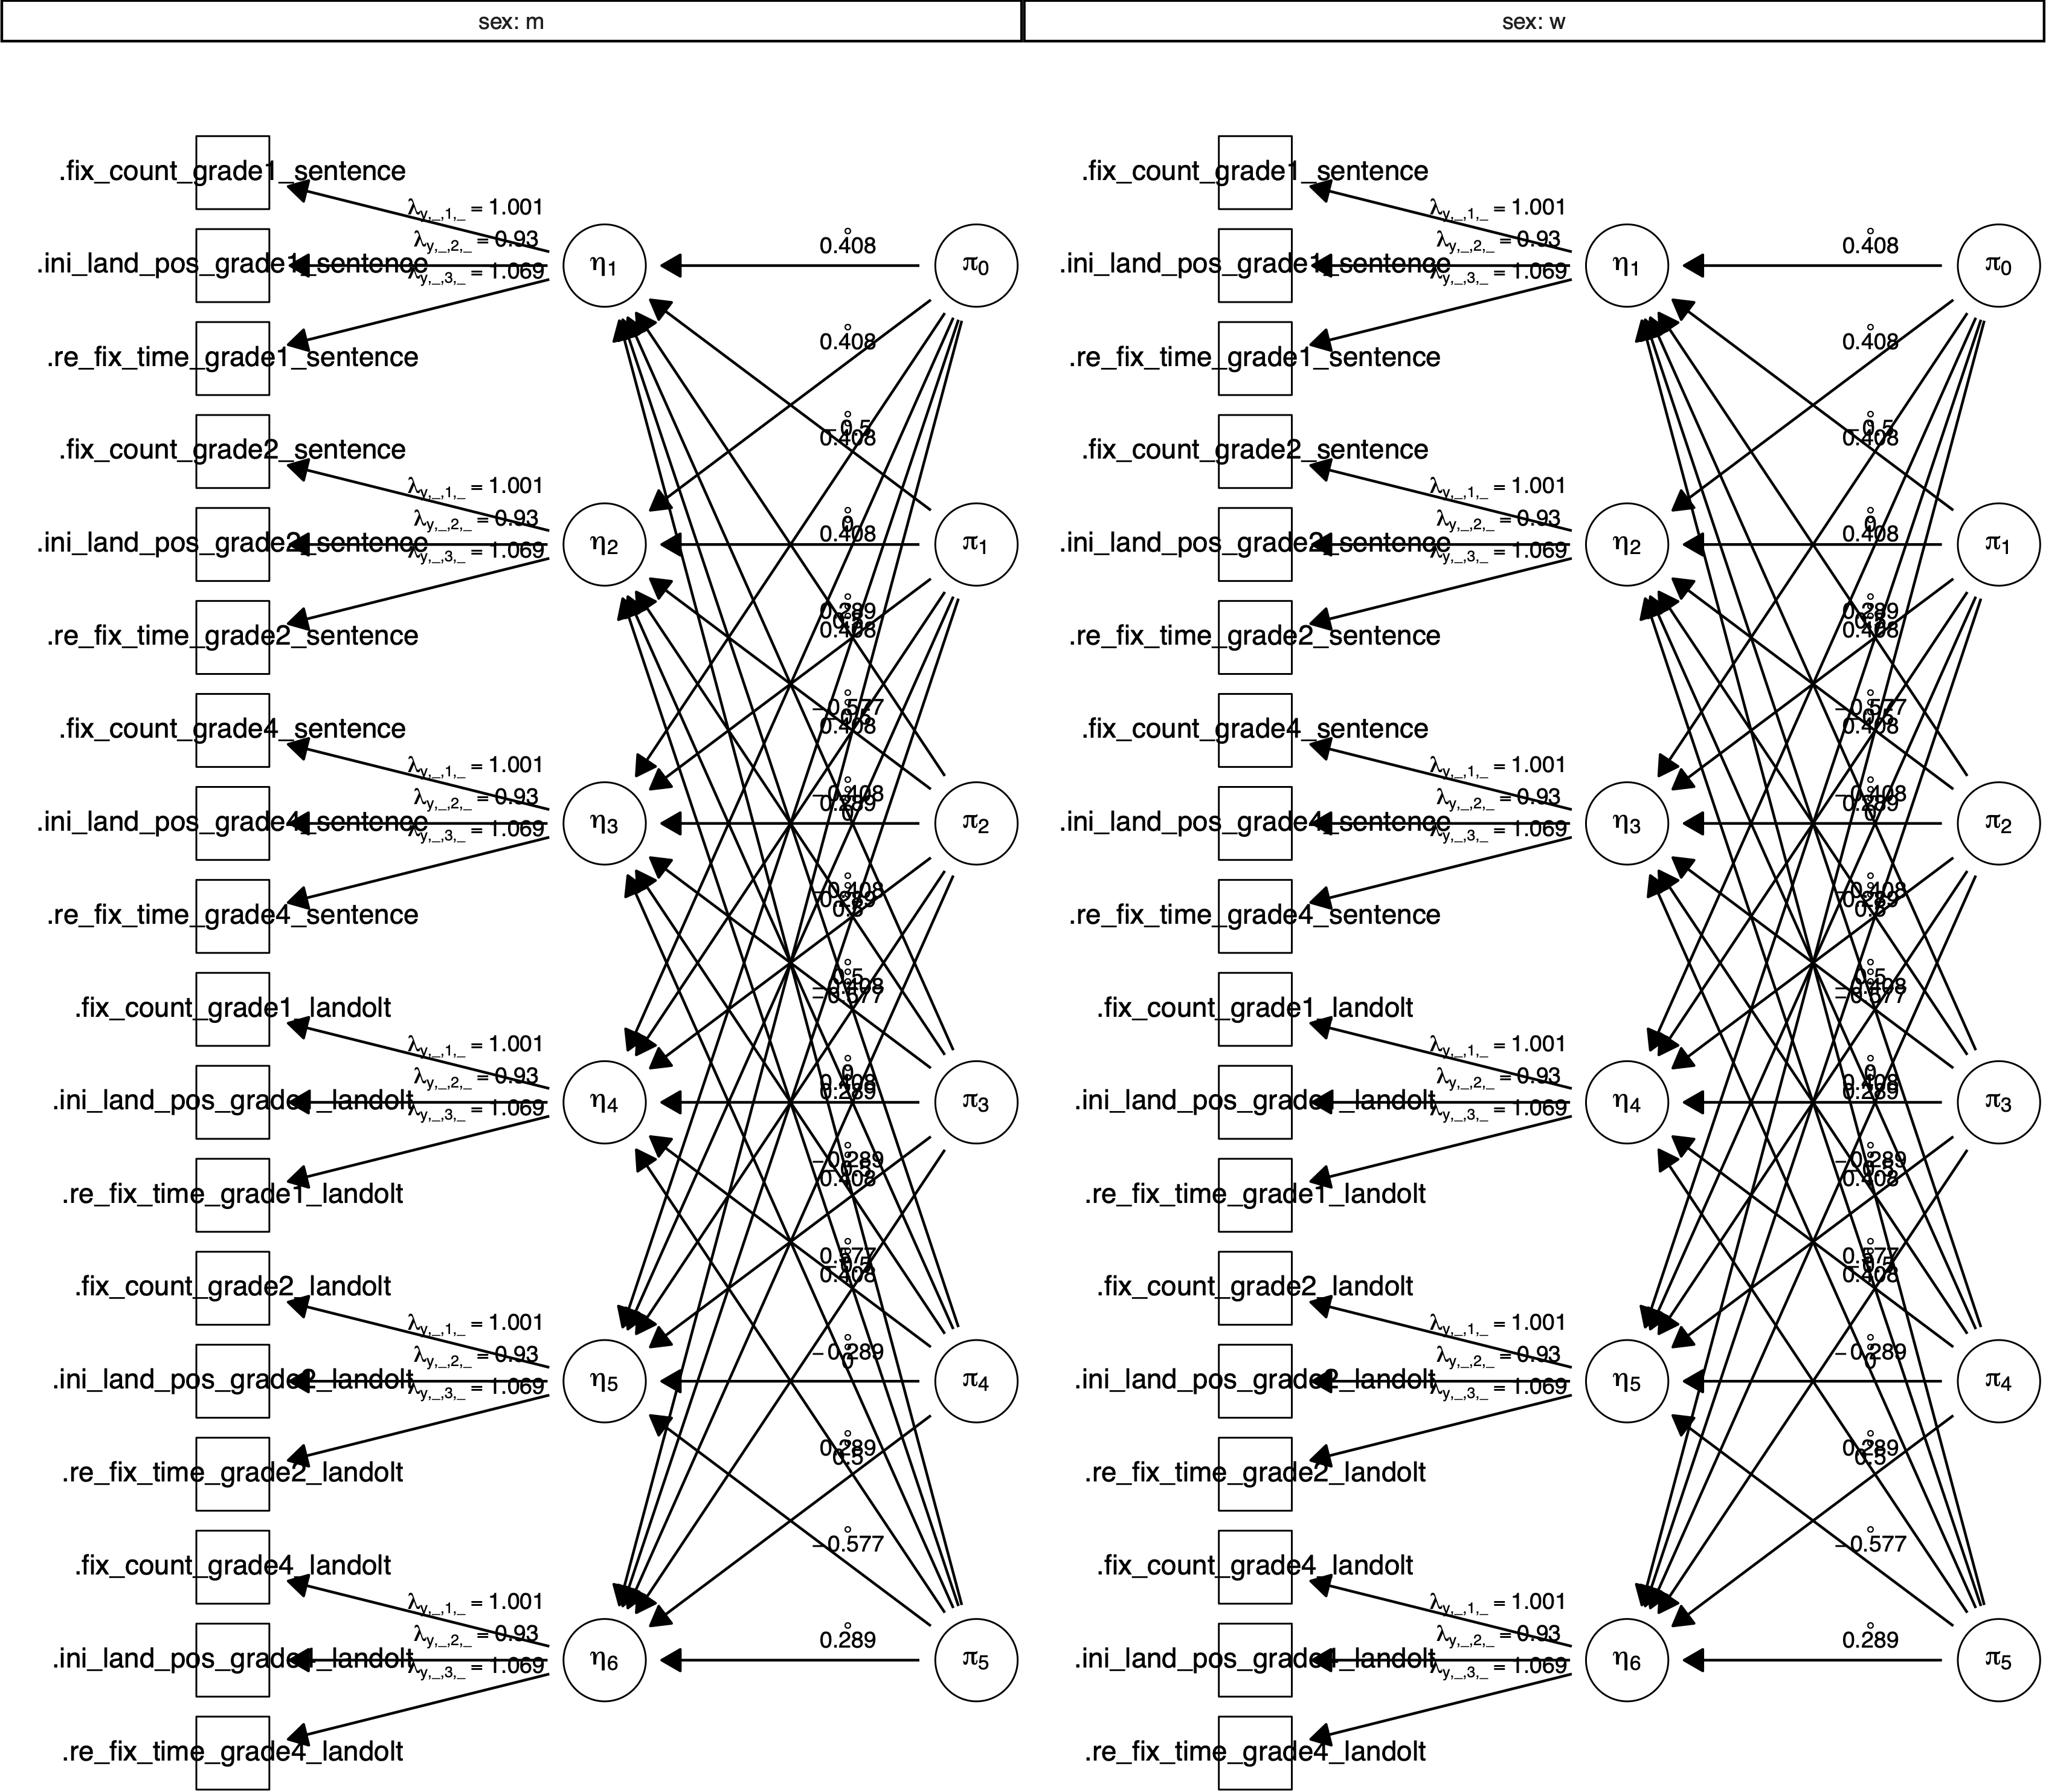
\includegraphics[width=1\linewidth]{semnova-man_files/figure-latex/software-between-latent-1} 

}

\caption{Path diagram created by \texttt{plot(fit\_btw\_latent)} for a $2 \times 3 \times 2$ (sentence $\times$ grade $\times$ sex) mixed design with the latent dependent variable reading ability measured by the three manifest variables re-fixation time, initial landing position and fixation count.}\label{fig:software-between-latent}
\end{figure}

\hypertarget{measurement-invariance-1}{%
\subsection{Measurement Invariance}\label{measurement-invariance-1}}

Measurement invariance must also be tested across groups. In order to be able to compare means between groups, strong measurement invariance is needed (i.e., equal loadings and intercepts between groups). This can be done by sequentially comparing models that assume different degrees of measurement invariance (i.e., configural, weak, strong, or strict). The \texttt{invariance\_between} argument can be set to \texttt{"configural"}, \texttt{"weak"}, \texttt{"strong"}, or \texttt{"strict"}.

\begin{Shaded}
\begin{Highlighting}[]
\NormalTok{fit\_btw\_latent\_configMI }\OtherTok{\textless{}{-}} \FunctionTok{semnova}\NormalTok{(}
    \AttributeTok{data =}\NormalTok{ reading\_latent,}
    \AttributeTok{id =} \StringTok{"id"}\NormalTok{, }
    \AttributeTok{dv =} \StringTok{"dv"}\NormalTok{,}
    \AttributeTok{indicator =} \StringTok{"indicator"}\NormalTok{,}
    \AttributeTok{equal\_resid\_cov =} \FunctionTok{list}\NormalTok{(}\StringTok{"ini\_land\_pos"}\NormalTok{, }\StringTok{"fix\_count"}\NormalTok{),}
    \AttributeTok{between =} \StringTok{"sex"}\NormalTok{,}
    \AttributeTok{within =} \FunctionTok{c}\NormalTok{(}\StringTok{"grade"}\NormalTok{, }\StringTok{"sentence"}\NormalTok{),}
    \AttributeTok{missing =} \StringTok{"fiml"}\NormalTok{,}
    \AttributeTok{invariance\_between =} \StringTok{"configural"}
\NormalTok{)}

\NormalTok{fit\_btw\_latent\_weakMI }\OtherTok{\textless{}{-}} \FunctionTok{semnova}\NormalTok{(}
    \AttributeTok{data =}\NormalTok{ reading\_latent,}
    \AttributeTok{id =} \StringTok{"id"}\NormalTok{, }
    \AttributeTok{dv =} \StringTok{"dv"}\NormalTok{,}
    \AttributeTok{indicator =} \StringTok{"indicator"}\NormalTok{,}
    \AttributeTok{equal\_resid\_cov =} \FunctionTok{list}\NormalTok{(}\StringTok{"ini\_land\_pos"}\NormalTok{, }\StringTok{"fix\_count"}\NormalTok{),}
    \AttributeTok{between =} \StringTok{"sex"}\NormalTok{,}
    \AttributeTok{within =} \FunctionTok{c}\NormalTok{(}\StringTok{"grade"}\NormalTok{, }\StringTok{"sentence"}\NormalTok{),}
    \AttributeTok{missing =} \StringTok{"fiml"}\NormalTok{,}
    \AttributeTok{invariance\_between =} \StringTok{"weak"}
\NormalTok{)}

\NormalTok{fit\_btw\_latent\_strongMI }\OtherTok{\textless{}{-}} \FunctionTok{semnova}\NormalTok{(}
    \AttributeTok{data =}\NormalTok{ reading\_latent,}
    \AttributeTok{id =} \StringTok{"id"}\NormalTok{, }
    \AttributeTok{dv =} \StringTok{"dv"}\NormalTok{,}
    \AttributeTok{indicator =} \StringTok{"indicator"}\NormalTok{,}
    \AttributeTok{equal\_resid\_cov =} \FunctionTok{list}\NormalTok{(}\StringTok{"ini\_land\_pos"}\NormalTok{, }\StringTok{"fix\_count"}\NormalTok{),}
    \AttributeTok{between =} \StringTok{"sex"}\NormalTok{,}
    \AttributeTok{within =} \FunctionTok{c}\NormalTok{(}\StringTok{"grade"}\NormalTok{, }\StringTok{"sentence"}\NormalTok{),}
    \AttributeTok{missing =} \StringTok{"fiml"}\NormalTok{,}
    \AttributeTok{invariance\_between =} \StringTok{"strong"}
\NormalTok{)}

\NormalTok{fit\_btw\_latent\_strictMI }\OtherTok{\textless{}{-}} \FunctionTok{semnova}\NormalTok{(}
    \AttributeTok{data =}\NormalTok{ reading\_latent,}
    \AttributeTok{id =} \StringTok{"id"}\NormalTok{, }
    \AttributeTok{dv =} \StringTok{"dv"}\NormalTok{,}
    \AttributeTok{indicator =} \StringTok{"indicator"}\NormalTok{,}
    \AttributeTok{equal\_resid\_cov =} \FunctionTok{list}\NormalTok{(}\StringTok{"ini\_land\_pos"}\NormalTok{, }\StringTok{"fix\_count"}\NormalTok{),}
    \AttributeTok{between =} \StringTok{"sex"}\NormalTok{,}
    \AttributeTok{within =} \FunctionTok{c}\NormalTok{(}\StringTok{"grade"}\NormalTok{, }\StringTok{"sentence"}\NormalTok{),}
    \AttributeTok{missing =} \StringTok{"fiml"}\NormalTok{,}
    \AttributeTok{invariance\_between =} \StringTok{"strict"}
\NormalTok{)}

\FunctionTok{anova}\NormalTok{(}
\NormalTok{    fit\_btw\_latent\_configMI, }
\NormalTok{    fit\_btw\_latent\_weakMI,}
\NormalTok{    fit\_btw\_latent\_strongMI,}
\NormalTok{    fit\_btw\_latent\_strictMI}
\NormalTok{)}
\end{Highlighting}
\end{Shaded}

\begin{verbatim}
## Chi-Squared Difference Test
## 
##                          Df    AIC    BIC  Chisq Chisq diff Df diff Pr(>Chisq)
## fit_btw_latent_configMI 272 5636.4 6016.6 686.14                              
## fit_btw_latent_weakMI   276 5633.9 5999.8 691.62      5.487       4     0.2408
## fit_btw_latent_strongMI 280 5627.5 5979.1 693.25      1.630       4     0.8034
## fit_btw_latent_strictMI 298 5677.5 5964.5 779.30     86.043      18  7.356e-11
##                            
## fit_btw_latent_configMI    
## fit_btw_latent_weakMI      
## fit_btw_latent_strongMI    
## fit_btw_latent_strictMI ***
## ---
## Signif. codes:  0 '***' 0.001 '**' 0.01 '*' 0.05 '.' 0.1 ' ' 1
\end{verbatim}

The fit of the first model is not very good. These results are in line with the results for the latent model from the previous examples. However, we can see that weak and strong measurement invariance explain the data equally well as compared to configural measurement invariance. The strict measurement invariance model, however, differs in terms of fit as compared to the other three models.

\hypertarget{covariates}{%
\chapter{Covariates}\label{covariates}}

The \texttt{semnova()} function can further incorporate manifest and latent covariates. The \texttt{covariates} argument takes a list of character vectors representing the variable names of covariates. If a character vector from the list consists of only one element, the covariate is treated as manifest, and as latent otherwise. If a manifest covariate points to a variable that contains a factor or characters, the variable will be dummy coded and included in the model. Interactions between manifest covariates will also be included. Interactions between latent covariates are not possible at this moment. Manifest variables measuring latent covariates must further be numerical.

In the next example, we estimate a \(2 \times 3\) within-subjects design for re-fixation time and include sex as a dummy-coded covariate and the latent covariate child behavior measured at the end of the study by the two scales \emph{internalizing} and \emph{externalizing} behavior. The scales are taken from the child behavior checklist \citep[CBLB,][]{Achenbach1991a}.

\begin{Shaded}
\begin{Highlighting}[]
\NormalTok{fit\_covariates }\OtherTok{\textless{}{-}} \FunctionTok{semnova}\NormalTok{(}
    \AttributeTok{data =}\NormalTok{ reading\_manifest,}
    \AttributeTok{id =} \StringTok{"id"}\NormalTok{, }
    \AttributeTok{dv =} \StringTok{"re\_fix\_time"}\NormalTok{,}
    \AttributeTok{within =} \FunctionTok{c}\NormalTok{(}\StringTok{"grade"}\NormalTok{, }\StringTok{"sentence"}\NormalTok{),}
    \AttributeTok{covariates =} \FunctionTok{list}\NormalTok{(}\StringTok{"sex"}\NormalTok{, }\AttributeTok{CBCL =} \FunctionTok{c}\NormalTok{(}\StringTok{"cbcl\_int\_verh\_rw\_t5"}\NormalTok{, }\StringTok{"cbcl\_ext\_verh\_rw\_t5"}\NormalTok{))}
\NormalTok{)}

\FunctionTok{summary}\NormalTok{(fit\_covariates)}
\end{Highlighting}
\end{Shaded}

\begin{verbatim}
## Fit measures:
## 
## Chisq(9) = 25.066, p = 0.003
## CFI = 0.962
## TLI = 0.847
## RMSEA = 0.107 [0.059, 0.158]
## 
## ##############################
## 
## Main and Interaction Effects:
##                       Chisq df Pr(>Chisq)    
## Intercept             1.105  1      0.293    
## grade               213.637  2     <2e-16 ***
## sentence            129.699  1     <2e-16 ***
## grade:sentence       57.760  2     <2e-16 ***
## sex                   0.002  1      0.964    
## grade:sex             2.263  2      0.323    
## sentence:sex          2.620  1      0.106    
## grade:sentence:sex    2.058  2      0.357    
## CBCL                  0.042  1      0.837    
## grade:CBCL            3.674  2      0.159    
## sentence:CBCL         0.257  1      0.612    
## grade:sentence:CBCL   2.648  2      0.266    
## ---
## Signif. codes:  0 '***' 0.001 '**' 0.01 '*' 0.05 '.' 0.1 ' ' 1
\end{verbatim}

Residual covariances between re-fixation time and the internalizing and externalizing child behavior are fixed to zero which explains the nine degrees of freedom. The fit is not perfect but can be considered satisfactory because the confidence interval of the root mean squared error of approximation (RMSEA) includes the established threshold of 0.06 \citep[e.g.,][]{Hu1999a}. Hypothesis tests for within-subjects factors are again significant. Effects involving the covariate sex are non-significant which is in line with the multi-group model from the previous sections. Effects involving child behavior are also non-significant. That is, child behavior does neither predict differences between genders nor does it predict differences in re-fixation time between grades or sentence types. Figure~\ref{fig:software-covariates} shows the path diagram of the model.

\begin{figure}

{\centering 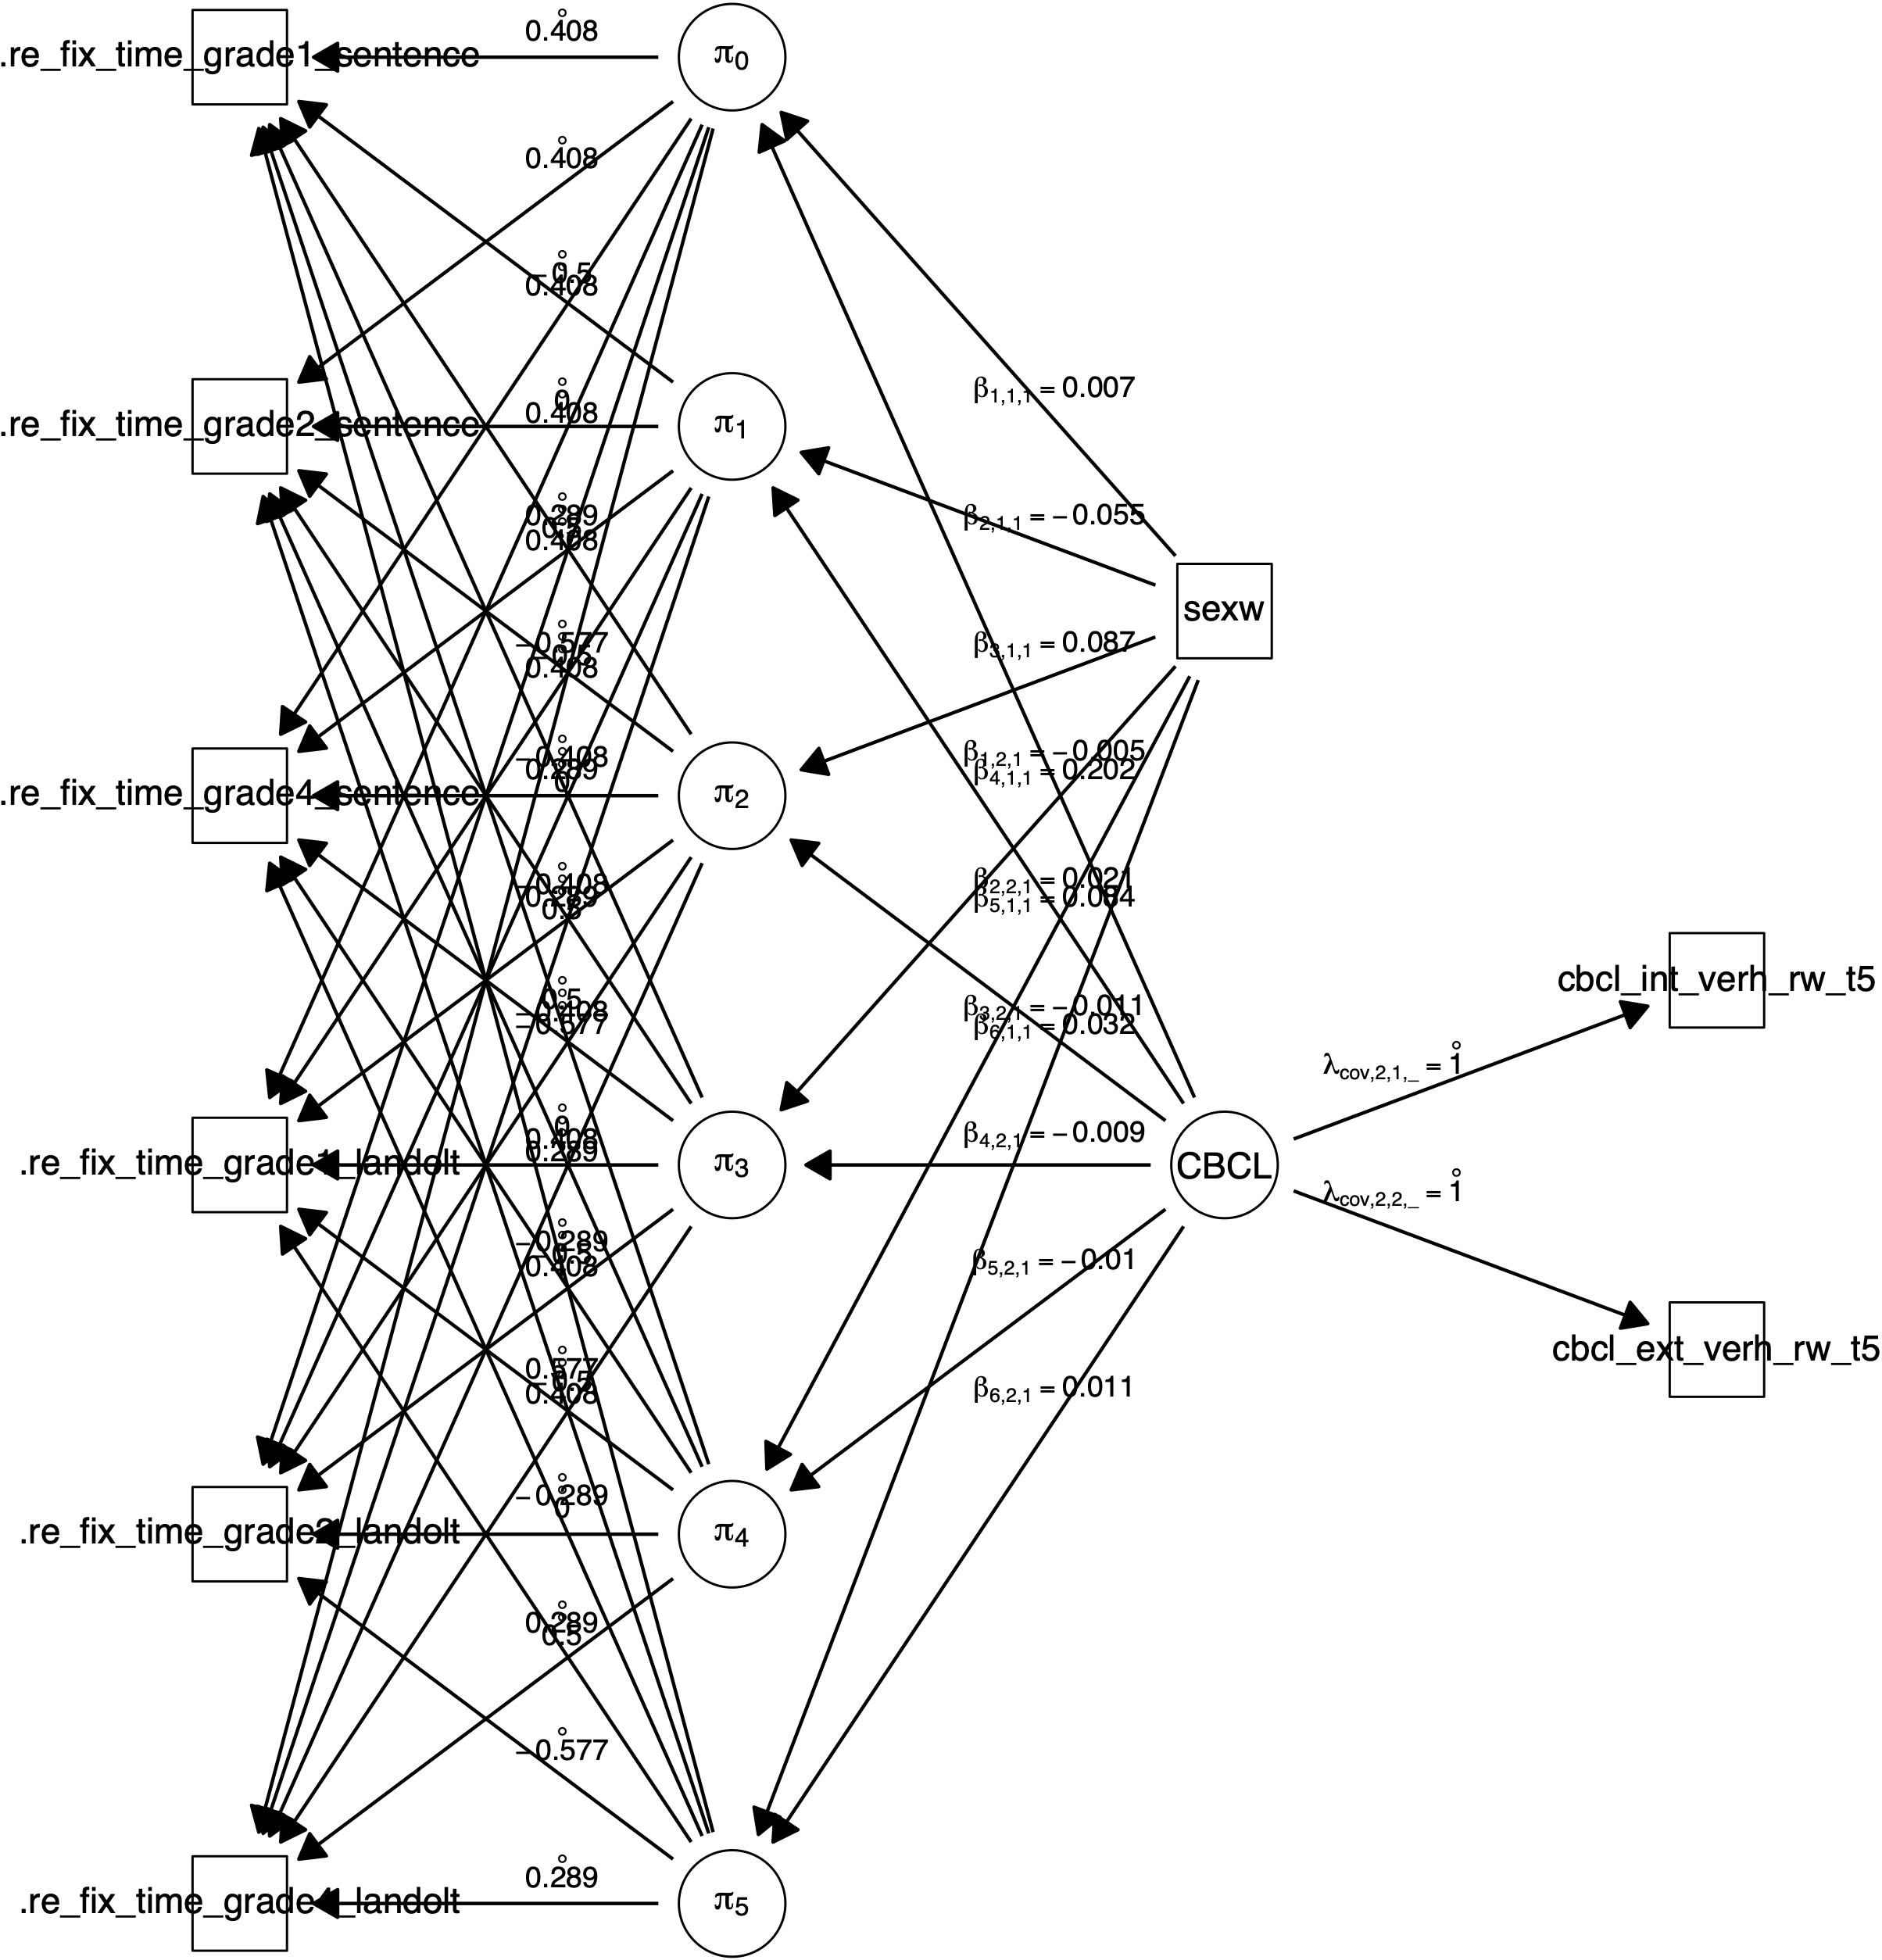
\includegraphics[width=1\linewidth]{semnova-man_files/figure-latex/software-covariates-1} 

}

\caption{Path diagram created by \texttt{plot(fit\_covariates)} for a $2    imes 3$ (sentence $ imes$ grade) within-subjects design with the manifest dependent variable re-fixation time, the manifest categorical covariate sex, and the latent covariate CBCL measured by the two manifest variables internalizing and externalizing child behavior.}\label{fig:software-covariates}
\end{figure}

\hypertarget{power-analysis}{%
\chapter{Power Analysis}\label{power-analysis}}

The \emph{semnova} package enables the researcher to perform power calculations for within- and between-subjects designs of any complexity. The \texttt{power\_script\_semnova()} function creates a script template making it very easy to specify population parameters in form of \emph{lavaan} model syntax. The \texttt{n\_within} argument takes an integer vector whose entries each represent a within-subjects factor with the number indicating the number of levels. \texttt{n\_between} takes the same input for the between-subjects design. \texttt{n\_indicator} takes a single integer representing the number of indicators. \texttt{n\_manifest\_covariates} takes the same input as \texttt{n\_within} and \texttt{n\_between}. However, if an entry equals one, the covariate is assumed to be continuous; if the entry is greater than or equal to two the covariate is assumed to be categorical with the number indicating the number of levels. \texttt{n\_latent\_covariates} take a vector of integers each representing a latent variable with the number indicating the number of manifest variables that measure the latent variable. Latent covariates are always assumed to be continuous. The \texttt{sphericity} argument takes a list of integer vectors and can be used to impose sphericity on effect variables of main or interaction effects. Each vector contains indices that refer to the within-subjects factors specified by \texttt{n\_within}. \texttt{out\_file} takes a path that the script file will be saved to.

What follows is an example for a \(2 \times 3 \times 2 \times 2\) (within \(\times\) within \(\times\) between \(\times\) between) mixed design with a latent dependent variable measured by three manifest variables, one continuous manifest covariate and one latent covariate measured by two manifest variables.

\begin{Shaded}
\begin{Highlighting}[]
\FunctionTok{power\_script\_semnova}\NormalTok{(}
    \AttributeTok{n\_within =} \FunctionTok{c}\NormalTok{(}\DecValTok{2}\NormalTok{,}\DecValTok{3}\NormalTok{),}
    \AttributeTok{n\_between =} \FunctionTok{c}\NormalTok{(}\DecValTok{2}\NormalTok{,}\DecValTok{2}\NormalTok{),}
    \AttributeTok{n\_indicator =} \DecValTok{3}\NormalTok{,}
    \AttributeTok{n\_manifest\_covariate =} \FunctionTok{c}\NormalTok{(}\DecValTok{1}\NormalTok{),}
    \AttributeTok{n\_latent\_covariate =} \FunctionTok{c}\NormalTok{(}\DecValTok{2}\NormalTok{),}
    \AttributeTok{out\_file =} \StringTok{"power\_script.R"}\NormalTok{,}
    \AttributeTok{sphericity =} \FunctionTok{list}\NormalTok{(}\FunctionTok{c}\NormalTok{(}\DecValTok{1}\NormalTok{,}\DecValTok{2}\NormalTok{))}
\NormalTok{)}
\end{Highlighting}
\end{Shaded}

The function will automatically name the factors, factor levels and covariates. Alternatively, the names can be given manually. The following code will produce exactly the same result as the previous example.

\begin{Shaded}
\begin{Highlighting}[]
\FunctionTok{power\_script\_semnova}\NormalTok{(}
    \AttributeTok{within =} \FunctionTok{list}\NormalTok{(}\FunctionTok{c}\NormalTok{(}\AttributeTok{W =} \FunctionTok{c}\NormalTok{(}\StringTok{"W1\_1"}\NormalTok{, }\StringTok{"W1\_2"}\NormalTok{), }\AttributeTok{W2 =} \FunctionTok{c}\NormalTok{(}\StringTok{"W2\_1"}\NormalTok{, }\StringTok{"W2\_2"}\NormalTok{, }\StringTok{"W2\_3"}\NormalTok{))),}
    \AttributeTok{between =} \FunctionTok{list}\NormalTok{(}\FunctionTok{c}\NormalTok{(}\AttributeTok{B =} \FunctionTok{c}\NormalTok{(}\StringTok{"B1\_1"}\NormalTok{, }\StringTok{"B1\_2"}\NormalTok{), }\AttributeTok{B2 =} \FunctionTok{c}\NormalTok{(}\StringTok{"B2\_1"}\NormalTok{, }\StringTok{"B2\_2"}\NormalTok{))),}
    \AttributeTok{indicator =} \FunctionTok{c}\NormalTok{(}\StringTok{"Y1"}\NormalTok{, }\StringTok{"Y2"}\NormalTok{, }\StringTok{"Y3"}\NormalTok{),}
    \AttributeTok{manifest\_covariate =} \FunctionTok{c}\NormalTok{(}\StringTok{"covariate1"}\NormalTok{),}
    \AttributeTok{latent\_covariate =} \FunctionTok{list}\NormalTok{(}\AttributeTok{covariate2 =} \FunctionTok{c}\NormalTok{(}\StringTok{"covariate2\_1"}\NormalTok{, }\StringTok{"covariate2\_1"}\NormalTok{)),}
    \AttributeTok{out\_file =} \StringTok{"power\_script.R"}\NormalTok{,}
    \AttributeTok{sphericity =} \FunctionTok{list}\NormalTok{(}\FunctionTok{c}\NormalTok{(}\StringTok{"W1"}\NormalTok{, }\StringTok{"W2"}\NormalTok{))}
\NormalTok{)}
\end{Highlighting}
\end{Shaded}

Within-subjects factors are automatically given the prefix \texttt{"W"}, between subjects factors have the prefix \texttt{"B"}, covariates begin with the word \texttt{"covariate"}, indicators of the dependent variables have the prefix \texttt{"Y"}, indicators of the covariates start with the covariate name.

The function \texttt{power\_script\_semnova()} will create a script file that consists of three main parts. First, the script contains a \emph{lavaan} model syntax that represents the specified model. The user has to replace parameter labels in the model syntax by population parameters. Second, the script contains a call to the \texttt{power\_analysis\_semnova()} function which will perform the power analysis and save the results to an object called \texttt{power}. The function takes the same input that was used to create the script file plus three additional parameters: \texttt{data\_syntax} takes the lavaan model syntax containing the population parameters; \texttt{sample\_size} takes a vector of sample sizes for the groups specified by the \texttt{n\_between} or \texttt{between} (the length of the vector must be one or equal to the number of groups); \texttt{replications} takes the number of replications for the power analysis. Third, the three functions \texttt{summary()}, \texttt{print()}, and \texttt{plot()} are suggested to extract information from the resulting object. The following code is the result from the previous call to \texttt{power\_script\_semnova} saved to the specified output file.

\begin{Shaded}
\begin{Highlighting}[]
\NormalTok{data\_syntax }\OtherTok{\textless{}{-}} \StringTok{"}
\StringTok{[...]}
\StringTok{"}

\NormalTok{power }\OtherTok{\textless{}{-}} \FunctionTok{power\_analysis\_semnova}\NormalTok{(}
    \AttributeTok{n\_within =} \FunctionTok{c}\NormalTok{(}\DecValTok{2}\NormalTok{, }\DecValTok{3}\NormalTok{),}
    \AttributeTok{n\_between =} \FunctionTok{c}\NormalTok{(}\DecValTok{2}\NormalTok{, }\DecValTok{2}\NormalTok{),}
    \AttributeTok{n\_indicator =} \DecValTok{3}\NormalTok{,}
    \AttributeTok{n\_manifest\_covariates =} \DecValTok{1}\NormalTok{,}
    \AttributeTok{n\_latent\_covariates =} \FunctionTok{c}\NormalTok{(}\DecValTok{2}\NormalTok{),}
    \AttributeTok{sphericity =} \FunctionTok{list}\NormalTok{(}\DecValTok{2}\NormalTok{),}
    \AttributeTok{data\_syntax =}\NormalTok{ data\_syntax,}
    \AttributeTok{sample\_size =} \FunctionTok{c}\NormalTok{(}\DecValTok{100}\NormalTok{, }\DecValTok{100}\NormalTok{, }\DecValTok{100}\NormalTok{, }\DecValTok{100}\NormalTok{),}
    \AttributeTok{replications =} \DecValTok{500}
\NormalTok{)}

\CommentTok{\# hypothesis tests}
\FunctionTok{summary}\NormalTok{(power)}

\CommentTok{\# parameters}
\FunctionTok{print}\NormalTok{(power)}

\CommentTok{\# path diagram}
\FunctionTok{plot}\NormalTok{(power)}
\end{Highlighting}
\end{Shaded}

The contents of the \texttt{data\_syntax} variable are omitted due to the large number of lines. The complete syntax can be found in \protect\hyperlink{power-script-example}{Appendix A}.

\protect\hyperlink{filled-power-script-example}{Appendix B} further contains a copy of the previously created power script filled with example population parameters. Means of latent variables and regression coefficients are set to 0.1. Variances of latent variables are set to 1 and covariances to 0.5. Loadings of manifest variables are set to 1 and intercepts to 0. Residual variances are 0.4 and residual covariances are set to 0.

Depending on the number of replications and the complexity of the model, the power analysis may need some time to finish. After the analysis, the \texttt{summary(power)} function can be used to print a table that contains the power for the main and interaction effects of the model. In the following output, the results are truncated after the sixth hypothesis.

\begin{verbatim}
## Table: Hypotheses
## 
## hypothesis                    power
## -----------------------  ----------
## B1                        0.0456349
## B1:B2                     0.0456349
## B1:B2:covariate1          0.0357143
## B1:B2:covariate2          0.0634921
## B1:covariate1             0.0515873
## B1:covariate2             0.0595238
## [...]
\end{verbatim}

We can further use the \texttt{print(power)} function to print the power and descriptive statistics for each of the model parameters separated by between-subjects factors (i.e., groups).

\begin{verbatim}
## Table: B1_1_B2_1
## 
## parameter                    mean          sd   pctNA       power       pct2.5        pct25       median       pct75     pct97.5
## --------------------  -----------  ----------  ------  ----------  -----------  -----------  -----------  ----------  ----------
## alpha_{pi,1,1}          0.0958489   0.1104171       0   0.1686508   -0.1392029    0.0188608    0.0999591   0.1698754   0.2996886
## alpha_{pi,2,1}          0.0977477   0.1118119       0   0.1666667   -0.1278233    0.0249539    0.0941303   0.1751148   0.3133758
## alpha_{pi,3,1}          0.0982346   0.1079209       0   0.1488095   -0.1170303    0.0220173    0.1044154   0.1701154   0.3070397
## alpha_{pi,4,1}          0.0994142   0.1099875       0   0.1428571   -0.1081087    0.0272029    0.1013290   0.1711141   0.3308732
## alpha_{pi,5,1}          0.1043942   0.1102061       0   0.1865079   -0.1095376    0.0330251    0.1028613   0.1854620   0.3055859
## alpha_{pi,6,1}          0.0997237   0.1035536       0   0.1329365   -0.0902241    0.0244948    0.1036009   0.1689088   0.2871981
## [...]
\end{verbatim}

Lastly, the \texttt{plot(power)} function plots a path diagram for the model. The diagram will include parameter labels but no estimates.

\begin{figure}

{\centering 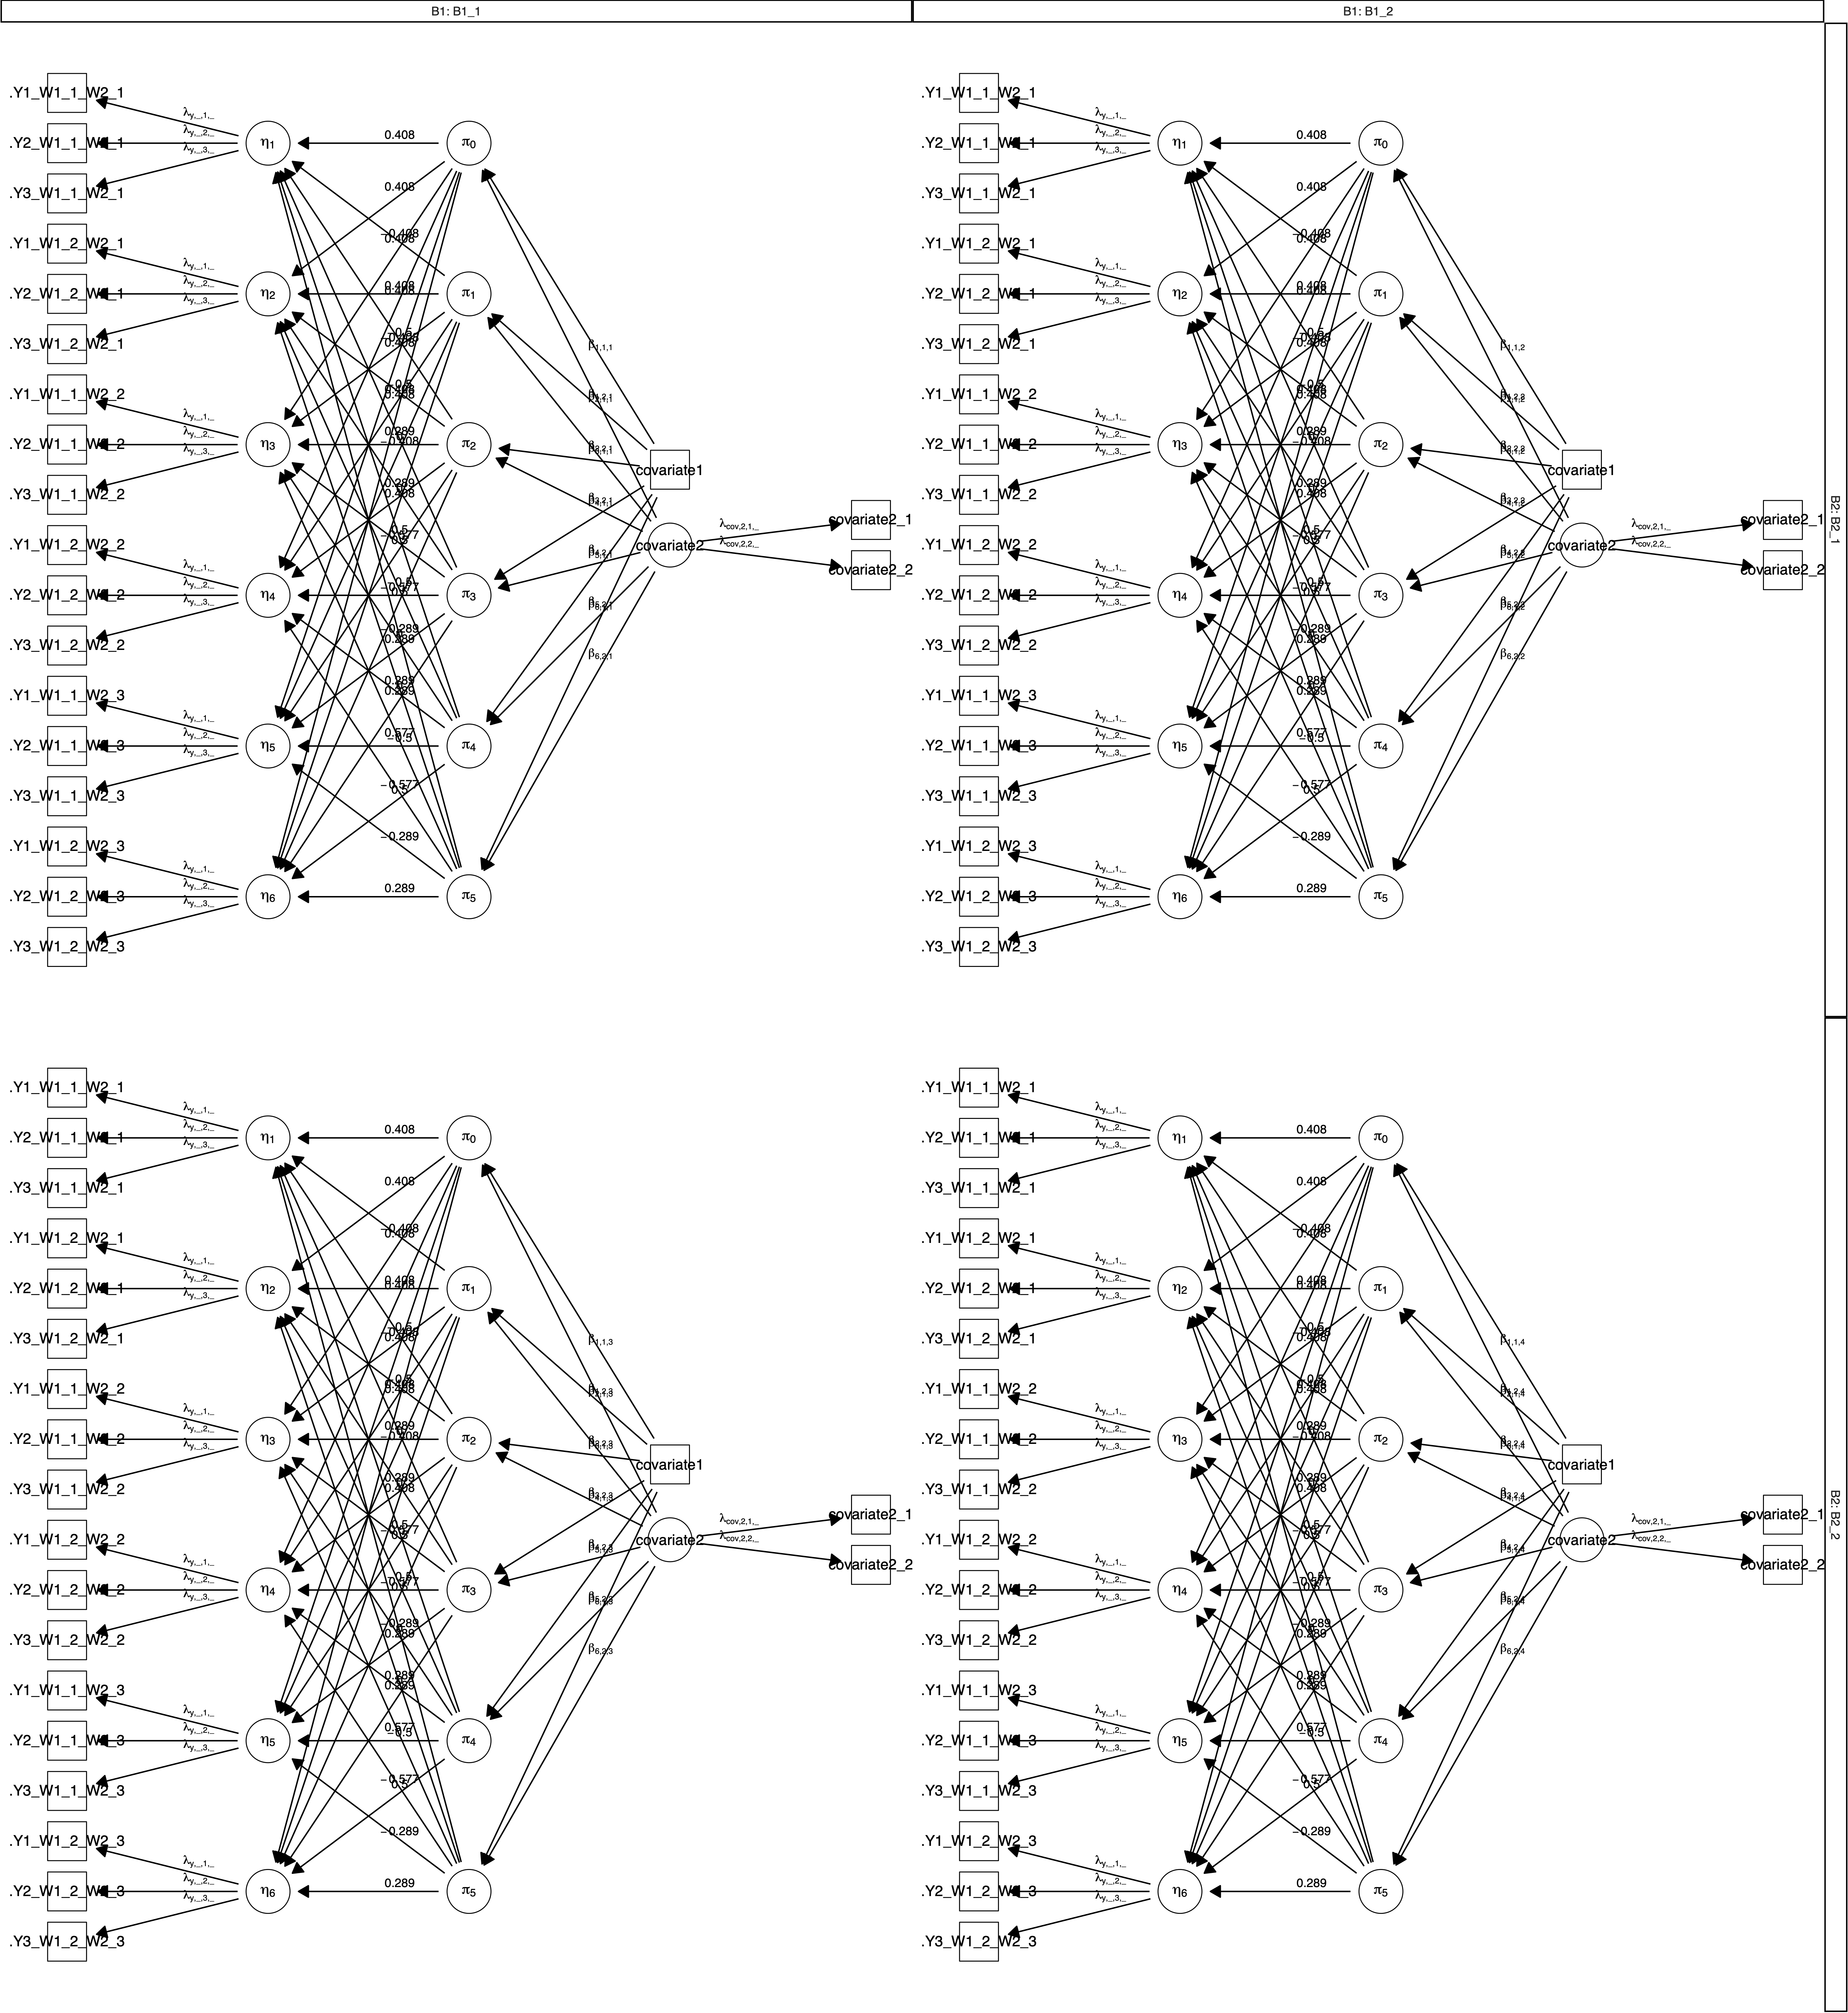
\includegraphics[width=1\linewidth]{semnova-man_files/figure-latex/software-power-1} 

}

\caption{Path diagram created by \texttt{plot(power)} for a $2  imes 3  imes 2  imes 2$ (within $   imes$ within $  imes$ between $ imes$ between) mixed design with a latent dependent variable, one manifest covariates, and one latent covariate measured by two manifest variables.}\label{fig:software-power}
\end{figure}

\hypertarget{further-arguments}{%
\chapter{Further Arguments}\label{further-arguments}}

The \texttt{semnova()} function accepts the following additional arguments which have not been described in this tutorial.

\begin{table}
\centering
\begin{tabular}{>{\raggedright\arraybackslash}p{0.3\textwidth}>{\raggedright\arraybackslash}p{0.7\textwidth}}
\toprule
\texttt{contrasts\_arg} & Named list that specifies the contrast coding scheme.\\
 & E.g.: \texttt{contrasts\_arg = list(grade = "contr.poly")}\\
\texttt{variance\_homogeneity} & Forces equal variances across groups. Can be used to test the assumption of variance homogeneity. Default is \texttt{FALSE}.\\
 & E.g.: \texttt{variance\_homogeneity = FALSE}\\
\texttt{lv\_scaling} & Specifies the latent variable identification scheme. Possible schemes are effect-code identification (\texttt{"effect"}, default) and referent-indicator identification (\texttt{"referent"}).\\
\addlinespace
 & E.g.: \texttt{lv\_scaling = "effect"}\\
\texttt{compound\_symmetry} & Forces the variances and covariances to be equal across the dependent variables. Can be used to test the assumption of compound symmetry. Default is \texttt{FALSE}.\\
 & E.g.: \texttt{compound\_symmetry = FALSE}\\
\texttt{normalize\_contrasts} & Scales the length of the contrasts to one. Default is \texttt{FALSE}.\\
 & E.g.: \texttt{normalize\_contrasts = FALSE}\\
\addlinespace
\texttt{append} & Appends the given character to the *lavaan* syntax.\\
 & E.g.: \texttt{append = "any lavaan syntax"}\\
\bottomrule
\end{tabular}
\end{table}

\hypertarget{further-developments}{%
\chapter{Further Developments}\label{further-developments}}

The \emph{semnova} package offers a wide range of features but remains work in progress. The road map for future developments is long and includes:

\begin{enumerate}
\def\labelenumi{\arabic{enumi}.}
\tightlist
\item
  Graphical user interface
\item
  Plotting features
\item
  Output for means and variances estimates
\item
  Output for effect size estimates
\item
  Average and conditional effects
\item
  Ordinal outcomes
\item
  Multilevel extension
\item
  Bayesian estimation
\item
  Different test statistics (e.g., likelihood ratio test, approximate \(F\)-test)
\end{enumerate}

\hypertarget{refs}{}
\begin{CSLReferences}{0}{0}
\end{CSLReferences}

\hypertarget{appendix-appendix}{%
\appendix}


\hypertarget{power-script-example}{%
\chapter{Power Script Example}\label{power-script-example}}

\begin{Shaded}
\begin{Highlighting}[]
\NormalTok{data\_syntax }\OtherTok{\textless{}{-}} \StringTok{"}
\StringTok{.eta1 =\textasciitilde{}}
\StringTok{    c(.lambda\_y\_\_1\_, .lambda\_y\_\_1\_, .lambda\_y\_\_1\_, .lambda\_y\_\_1\_)*.Y1\_W1\_1\_W2\_1 +}
\StringTok{    c(.lambda\_y\_\_2\_, .lambda\_y\_\_2\_, .lambda\_y\_\_2\_, .lambda\_y\_\_2\_)*.Y2\_W1\_1\_W2\_1 +}
\StringTok{    c(.lambda\_y\_\_3\_, .lambda\_y\_\_3\_, .lambda\_y\_\_3\_, .lambda\_y\_\_3\_)*.Y3\_W1\_1\_W2\_1}
\StringTok{.eta2 =\textasciitilde{}}
\StringTok{    c(.lambda\_y\_\_1\_, .lambda\_y\_\_1\_, .lambda\_y\_\_1\_, .lambda\_y\_\_1\_)*.Y1\_W1\_2\_W2\_1 +}
\StringTok{    c(.lambda\_y\_\_2\_, .lambda\_y\_\_2\_, .lambda\_y\_\_2\_, .lambda\_y\_\_2\_)*.Y2\_W1\_2\_W2\_1 +}
\StringTok{    c(.lambda\_y\_\_3\_, .lambda\_y\_\_3\_, .lambda\_y\_\_3\_, .lambda\_y\_\_3\_)*.Y3\_W1\_2\_W2\_1}
\StringTok{.eta3 =\textasciitilde{}}
\StringTok{    c(.lambda\_y\_\_1\_, .lambda\_y\_\_1\_, .lambda\_y\_\_1\_, .lambda\_y\_\_1\_)*.Y1\_W1\_1\_W2\_2 +}
\StringTok{    c(.lambda\_y\_\_2\_, .lambda\_y\_\_2\_, .lambda\_y\_\_2\_, .lambda\_y\_\_2\_)*.Y2\_W1\_1\_W2\_2 +}
\StringTok{    c(.lambda\_y\_\_3\_, .lambda\_y\_\_3\_, .lambda\_y\_\_3\_, .lambda\_y\_\_3\_)*.Y3\_W1\_1\_W2\_2}
\StringTok{.eta4 =\textasciitilde{}}
\StringTok{    c(.lambda\_y\_\_1\_, .lambda\_y\_\_1\_, .lambda\_y\_\_1\_, .lambda\_y\_\_1\_)*.Y1\_W1\_2\_W2\_2 +}
\StringTok{    c(.lambda\_y\_\_2\_, .lambda\_y\_\_2\_, .lambda\_y\_\_2\_, .lambda\_y\_\_2\_)*.Y2\_W1\_2\_W2\_2 +}
\StringTok{    c(.lambda\_y\_\_3\_, .lambda\_y\_\_3\_, .lambda\_y\_\_3\_, .lambda\_y\_\_3\_)*.Y3\_W1\_2\_W2\_2}
\StringTok{.eta5 =\textasciitilde{}}
\StringTok{    c(.lambda\_y\_\_1\_, .lambda\_y\_\_1\_, .lambda\_y\_\_1\_, .lambda\_y\_\_1\_)*.Y1\_W1\_1\_W2\_3 +}
\StringTok{    c(.lambda\_y\_\_2\_, .lambda\_y\_\_2\_, .lambda\_y\_\_2\_, .lambda\_y\_\_2\_)*.Y2\_W1\_1\_W2\_3 +}
\StringTok{    c(.lambda\_y\_\_3\_, .lambda\_y\_\_3\_, .lambda\_y\_\_3\_, .lambda\_y\_\_3\_)*.Y3\_W1\_1\_W2\_3}
\StringTok{.eta6 =\textasciitilde{}}
\StringTok{    c(.lambda\_y\_\_1\_, .lambda\_y\_\_1\_, .lambda\_y\_\_1\_, .lambda\_y\_\_1\_)*.Y1\_W1\_2\_W2\_3 +}
\StringTok{    c(.lambda\_y\_\_2\_, .lambda\_y\_\_2\_, .lambda\_y\_\_2\_, .lambda\_y\_\_2\_)*.Y2\_W1\_2\_W2\_3 +}
\StringTok{    c(.lambda\_y\_\_3\_, .lambda\_y\_\_3\_, .lambda\_y\_\_3\_, .lambda\_y\_\_3\_)*.Y3\_W1\_2\_W2\_3}
\StringTok{.pi1 =\textasciitilde{}}
\StringTok{    c(1, 1, 1, 1)*.eta1 +}
\StringTok{    c(1, 1, 1, 1)*.eta2 +}
\StringTok{    c(1, 1, 1, 1)*.eta3 +}
\StringTok{    c(1, 1, 1, 1)*.eta4 +}
\StringTok{    c(1, 1, 1, 1)*.eta5 +}
\StringTok{    c(1, 1, 1, 1)*.eta6}
\StringTok{.pi2 =\textasciitilde{}}
\StringTok{    c({-}0.707106781186547, {-}0.707106781186547, {-}0.707106781186547, {-}0.707106781186547)*.eta1 +}
\StringTok{    c(0.707106781186547, 0.707106781186547, 0.707106781186547, 0.707106781186547)*.eta2 +}
\StringTok{    c({-}0.707106781186547, {-}0.707106781186547, {-}0.707106781186547, {-}0.707106781186547)*.eta3 +}
\StringTok{    c(0.707106781186547, 0.707106781186547, 0.707106781186547, 0.707106781186547)*.eta4 +}
\StringTok{    c({-}0.707106781186547, {-}0.707106781186547, {-}0.707106781186547, {-}0.707106781186547)*.eta5 +}
\StringTok{    c(0.707106781186547, 0.707106781186547, 0.707106781186547, 0.707106781186547)*.eta6}
\StringTok{.pi3 =\textasciitilde{}}
\StringTok{    c({-}0.707106781186548, {-}0.707106781186548, {-}0.707106781186548, {-}0.707106781186548)*.eta1 +}
\StringTok{    c({-}0.707106781186548, {-}0.707106781186548, {-}0.707106781186548, {-}0.707106781186548)*.eta2 +}
\StringTok{    c(0, 0, 0, 0)*.eta3 +}
\StringTok{    c(0, 0, 0, 0)*.eta4 +}
\StringTok{    c(0.707106781186547, 0.707106781186547, 0.707106781186547, 0.707106781186547)*.eta5 +}
\StringTok{    c(0.707106781186547, 0.707106781186547, 0.707106781186547, 0.707106781186547)*.eta6}
\StringTok{.pi4 =\textasciitilde{}}
\StringTok{    c(0.408248290463863, 0.408248290463863, 0.408248290463863, 0.408248290463863)*.eta1 +}
\StringTok{    c(0.408248290463863, 0.408248290463863, 0.408248290463863, 0.408248290463863)*.eta2 +}
\StringTok{    c({-}0.816496580927726, {-}0.816496580927726, {-}0.816496580927726, {-}0.816496580927726)*.eta3 +}
\StringTok{    c({-}0.816496580927726, {-}0.816496580927726, {-}0.816496580927726, {-}0.816496580927726)*.eta4 +}
\StringTok{    c(0.408248290463863, 0.408248290463863, 0.408248290463863, 0.408248290463863)*.eta5 +}
\StringTok{    c(0.408248290463863, 0.408248290463863, 0.408248290463863, 0.408248290463863)*.eta6}
\StringTok{.pi5 =\textasciitilde{}}
\StringTok{    c(0.5, 0.5, 0.5, 0.5)*.eta1 +}
\StringTok{    c({-}0.5, {-}0.5, {-}0.5, {-}0.5)*.eta2 +}
\StringTok{    c(0, 0, 0, 0)*.eta3 +}
\StringTok{    c(0, 0, 0, 0)*.eta4 +}
\StringTok{    c({-}0.5, {-}0.5, {-}0.5, {-}0.5)*.eta5 +}
\StringTok{    c(0.5, 0.5, 0.5, 0.5)*.eta6}
\StringTok{.pi6 =\textasciitilde{}}
\StringTok{    c({-}0.288675134594813, {-}0.288675134594813, {-}0.288675134594813, {-}0.288675134594813)*.eta1 +}
\StringTok{    c(0.288675134594813, 0.288675134594813, 0.288675134594813, 0.288675134594813)*.eta2 +}
\StringTok{    c(0.577350269189626, 0.577350269189626, 0.577350269189626, 0.577350269189626)*.eta3 +}
\StringTok{    c({-}0.577350269189626, {-}0.577350269189626, {-}0.577350269189626, {-}0.577350269189626)*.eta4 +}
\StringTok{    c({-}0.288675134594813, {-}0.288675134594813, {-}0.288675134594813, {-}0.288675134594813)*.eta5 +}
\StringTok{    c(0.288675134594813, 0.288675134594813, 0.288675134594813, 0.288675134594813)*.eta6}
\StringTok{covariate2 =\textasciitilde{}}
\StringTok{    c(.lambda\_cov\_2\_1\_, .lambda\_cov\_2\_1\_, .lambda\_cov\_2\_1\_, .lambda\_cov\_2\_1\_)*covariate2\_1 +}
\StringTok{    c(.lambda\_cov\_2\_2\_, .lambda\_cov\_2\_2\_, .lambda\_cov\_2\_2\_, .lambda\_cov\_2\_2\_)*covariate2\_2}
\StringTok{.pi1 \textasciitilde{}}
\StringTok{    c(.beta\_1\_1\_1, .beta\_1\_1\_2, .beta\_1\_1\_3, .beta\_1\_1\_4)*covariate1 +}
\StringTok{    c(.beta\_1\_2\_1, .beta\_1\_2\_2, .beta\_1\_2\_3, .beta\_1\_2\_4)*covariate2}
\StringTok{.pi2 \textasciitilde{}}
\StringTok{    c(.beta\_2\_1\_1, .beta\_2\_1\_2, .beta\_2\_1\_3, .beta\_2\_1\_4)*covariate1 +}
\StringTok{    c(.beta\_2\_2\_1, .beta\_2\_2\_2, .beta\_2\_2\_3, .beta\_2\_2\_4)*covariate2}
\StringTok{.pi3 \textasciitilde{}}
\StringTok{    c(.beta\_3\_1\_1, .beta\_3\_1\_2, .beta\_3\_1\_3, .beta\_3\_1\_4)*covariate1 +}
\StringTok{    c(.beta\_3\_2\_1, .beta\_3\_2\_2, .beta\_3\_2\_3, .beta\_3\_2\_4)*covariate2}
\StringTok{.pi4 \textasciitilde{}}
\StringTok{    c(.beta\_4\_1\_1, .beta\_4\_1\_2, .beta\_4\_1\_3, .beta\_4\_1\_4)*covariate1 +}
\StringTok{    c(.beta\_4\_2\_1, .beta\_4\_2\_2, .beta\_4\_2\_3, .beta\_4\_2\_4)*covariate2}
\StringTok{.pi5 \textasciitilde{}}
\StringTok{    c(.beta\_5\_1\_1, .beta\_5\_1\_2, .beta\_5\_1\_3, .beta\_5\_1\_4)*covariate1 +}
\StringTok{    c(.beta\_5\_2\_1, .beta\_5\_2\_2, .beta\_5\_2\_3, .beta\_5\_2\_4)*covariate2}
\StringTok{.pi6 \textasciitilde{}}
\StringTok{    c(.beta\_6\_1\_1, .beta\_6\_1\_2, .beta\_6\_1\_3, .beta\_6\_1\_4)*covariate1 +}
\StringTok{    c(.beta\_6\_2\_1, .beta\_6\_2\_2, .beta\_6\_2\_3, .beta\_6\_2\_4)*covariate2}
\StringTok{.eta1 \textasciitilde{}\textasciitilde{}}
\StringTok{    c(0, 0, 0, 0)*.eta1 +}
\StringTok{    c(0, 0, 0, 0)*.eta2 +}
\StringTok{    c(0, 0, 0, 0)*.eta3 +}
\StringTok{    c(0, 0, 0, 0)*.eta4 +}
\StringTok{    c(0, 0, 0, 0)*.eta5 +}
\StringTok{    c(0, 0, 0, 0)*.eta6}
\StringTok{.eta2 \textasciitilde{}\textasciitilde{}}
\StringTok{    c(0, 0, 0, 0)*.eta2 +}
\StringTok{    c(0, 0, 0, 0)*.eta3 +}
\StringTok{    c(0, 0, 0, 0)*.eta4 +}
\StringTok{    c(0, 0, 0, 0)*.eta5 +}
\StringTok{    c(0, 0, 0, 0)*.eta6}
\StringTok{.eta3 \textasciitilde{}\textasciitilde{}}
\StringTok{    c(0, 0, 0, 0)*.eta3 +}
\StringTok{    c(0, 0, 0, 0)*.eta4 +}
\StringTok{    c(0, 0, 0, 0)*.eta5 +}
\StringTok{    c(0, 0, 0, 0)*.eta6}
\StringTok{.eta4 \textasciitilde{}\textasciitilde{}}
\StringTok{    c(0, 0, 0, 0)*.eta4 +}
\StringTok{    c(0, 0, 0, 0)*.eta5 +}
\StringTok{    c(0, 0, 0, 0)*.eta6}
\StringTok{.eta5 \textasciitilde{}\textasciitilde{}}
\StringTok{    c(0, 0, 0, 0)*.eta5 +}
\StringTok{    c(0, 0, 0, 0)*.eta6}
\StringTok{.eta6 \textasciitilde{}\textasciitilde{}}
\StringTok{    c(0, 0, 0, 0)*.eta6}
\StringTok{.pi1 \textasciitilde{}\textasciitilde{}}
\StringTok{    c(.sigma\_pi\_1\_1\_1, .sigma\_pi\_1\_1\_2, .sigma\_pi\_1\_1\_3, .sigma\_pi\_1\_1\_4)*.pi1 +}
\StringTok{    c(.sigma\_pi\_1\_2\_1, .sigma\_pi\_1\_2\_2, .sigma\_pi\_1\_2\_3, .sigma\_pi\_1\_2\_4)*.pi2 +}
\StringTok{    c(.sigma\_pi\_1\_3\_1, .sigma\_pi\_1\_3\_2, .sigma\_pi\_1\_3\_3, .sigma\_pi\_1\_3\_4)*.pi3 +}
\StringTok{    c(.sigma\_pi\_1\_4\_1, .sigma\_pi\_1\_4\_2, .sigma\_pi\_1\_4\_3, .sigma\_pi\_1\_4\_4)*.pi4 +}
\StringTok{    c(.sigma\_pi\_1\_5\_1, .sigma\_pi\_1\_5\_2, .sigma\_pi\_1\_5\_3, .sigma\_pi\_1\_5\_4)*.pi5 +}
\StringTok{    c(.sigma\_pi\_1\_6\_1, .sigma\_pi\_1\_6\_2, .sigma\_pi\_1\_6\_3, .sigma\_pi\_1\_6\_4)*.pi6}
\StringTok{.pi2 \textasciitilde{}\textasciitilde{}}
\StringTok{    c(.sigma\_pi\_2\_2\_1, .sigma\_pi\_2\_2\_2, .sigma\_pi\_2\_2\_3, .sigma\_pi\_2\_2\_4)*.pi2 +}
\StringTok{    c(.sigma\_pi\_2\_3\_1, .sigma\_pi\_2\_3\_2, .sigma\_pi\_2\_3\_3, .sigma\_pi\_2\_3\_4)*.pi3 +}
\StringTok{    c(.sigma\_pi\_2\_4\_1, .sigma\_pi\_2\_4\_2, .sigma\_pi\_2\_4\_3, .sigma\_pi\_2\_4\_4)*.pi4 +}
\StringTok{    c(.sigma\_pi\_2\_5\_1, .sigma\_pi\_2\_5\_2, .sigma\_pi\_2\_5\_3, .sigma\_pi\_2\_5\_4)*.pi5 +}
\StringTok{    c(.sigma\_pi\_2\_6\_1, .sigma\_pi\_2\_6\_2, .sigma\_pi\_2\_6\_3, .sigma\_pi\_2\_6\_4)*.pi6}
\StringTok{.pi3 \textasciitilde{}\textasciitilde{}}
\StringTok{    c(.sigma\_pi\_1\_\_1, .sigma\_pi\_1\_\_2, .sigma\_pi\_1\_\_3, .sigma\_pi\_1\_\_4)*.pi3 +}
\StringTok{    c(0, 0, 0, 0)*.pi4 +}
\StringTok{    c(.sigma\_pi\_3\_5\_1, .sigma\_pi\_3\_5\_2, .sigma\_pi\_3\_5\_3, .sigma\_pi\_3\_5\_4)*.pi5 +}
\StringTok{    c(.sigma\_pi\_3\_6\_1, .sigma\_pi\_3\_6\_2, .sigma\_pi\_3\_6\_3, .sigma\_pi\_3\_6\_4)*.pi6}
\StringTok{.pi4 \textasciitilde{}\textasciitilde{}}
\StringTok{    c(.sigma\_pi\_1\_\_1, .sigma\_pi\_1\_\_2, .sigma\_pi\_1\_\_3, .sigma\_pi\_1\_\_4)*.pi4 +}
\StringTok{    c(.sigma\_pi\_4\_5\_1, .sigma\_pi\_4\_5\_2, .sigma\_pi\_4\_5\_3, .sigma\_pi\_4\_5\_4)*.pi5 +}
\StringTok{    c(.sigma\_pi\_4\_6\_1, .sigma\_pi\_4\_6\_2, .sigma\_pi\_4\_6\_3, .sigma\_pi\_4\_6\_4)*.pi6}
\StringTok{.pi5 \textasciitilde{}\textasciitilde{}}
\StringTok{    c(.sigma\_pi\_5\_5\_1, .sigma\_pi\_5\_5\_2, .sigma\_pi\_5\_5\_3, .sigma\_pi\_5\_5\_4)*.pi5 +}
\StringTok{    c(.sigma\_pi\_5\_6\_1, .sigma\_pi\_5\_6\_2, .sigma\_pi\_5\_6\_3, .sigma\_pi\_5\_6\_4)*.pi6}
\StringTok{.pi6 \textasciitilde{}\textasciitilde{}}
\StringTok{    c(.sigma\_pi\_6\_6\_1, .sigma\_pi\_6\_6\_2, .sigma\_pi\_6\_6\_3, .sigma\_pi\_6\_6\_4)*.pi6}
\StringTok{.Y1\_W1\_1\_W2\_1 \textasciitilde{}\textasciitilde{}}
\StringTok{    c(.epsilon\_y\_1\_1\_1, .epsilon\_y\_1\_1\_2, .epsilon\_y\_1\_1\_3, .epsilon\_y\_1\_1\_4)*.Y1\_W1\_1\_W2\_1}
\StringTok{.Y1\_W1\_1\_W2\_2 \textasciitilde{}\textasciitilde{}}
\StringTok{    c(.epsilon\_y\_3\_1\_1, .epsilon\_y\_3\_1\_2, .epsilon\_y\_3\_1\_3, .epsilon\_y\_3\_1\_4)*.Y1\_W1\_1\_W2\_2}
\StringTok{.Y1\_W1\_1\_W2\_3 \textasciitilde{}\textasciitilde{}}
\StringTok{    c(.epsilon\_y\_5\_1\_1, .epsilon\_y\_5\_1\_2, .epsilon\_y\_5\_1\_3, .epsilon\_y\_5\_1\_4)*.Y1\_W1\_1\_W2\_3}
\StringTok{.Y1\_W1\_2\_W2\_1 \textasciitilde{}\textasciitilde{}}
\StringTok{    c(.epsilon\_y\_2\_1\_1, .epsilon\_y\_2\_1\_2, .epsilon\_y\_2\_1\_3, .epsilon\_y\_2\_1\_4)*.Y1\_W1\_2\_W2\_1}
\StringTok{.Y1\_W1\_2\_W2\_2 \textasciitilde{}\textasciitilde{}}
\StringTok{    c(.epsilon\_y\_4\_1\_1, .epsilon\_y\_4\_1\_2, .epsilon\_y\_4\_1\_3, .epsilon\_y\_4\_1\_4)*.Y1\_W1\_2\_W2\_2}
\StringTok{.Y1\_W1\_2\_W2\_3 \textasciitilde{}\textasciitilde{}}
\StringTok{    c(.epsilon\_y\_6\_1\_1, .epsilon\_y\_6\_1\_2, .epsilon\_y\_6\_1\_3, .epsilon\_y\_6\_1\_4)*.Y1\_W1\_2\_W2\_3}
\StringTok{.Y2\_W1\_1\_W2\_1 \textasciitilde{}\textasciitilde{}}
\StringTok{    c(.epsilon\_y\_1\_2\_1, .epsilon\_y\_1\_2\_2, .epsilon\_y\_1\_2\_3, .epsilon\_y\_1\_2\_4)*.Y2\_W1\_1\_W2\_1}
\StringTok{.Y2\_W1\_1\_W2\_2 \textasciitilde{}\textasciitilde{}}
\StringTok{    c(.epsilon\_y\_3\_2\_1, .epsilon\_y\_3\_2\_2, .epsilon\_y\_3\_2\_3, .epsilon\_y\_3\_2\_4)*.Y2\_W1\_1\_W2\_2}
\StringTok{.Y2\_W1\_1\_W2\_3 \textasciitilde{}\textasciitilde{}}
\StringTok{    c(.epsilon\_y\_5\_2\_1, .epsilon\_y\_5\_2\_2, .epsilon\_y\_5\_2\_3, .epsilon\_y\_5\_2\_4)*.Y2\_W1\_1\_W2\_3}
\StringTok{.Y2\_W1\_2\_W2\_1 \textasciitilde{}\textasciitilde{}}
\StringTok{    c(.epsilon\_y\_2\_2\_1, .epsilon\_y\_2\_2\_2, .epsilon\_y\_2\_2\_3, .epsilon\_y\_2\_2\_4)*.Y2\_W1\_2\_W2\_1}
\StringTok{.Y2\_W1\_2\_W2\_2 \textasciitilde{}\textasciitilde{}}
\StringTok{    c(.epsilon\_y\_4\_2\_1, .epsilon\_y\_4\_2\_2, .epsilon\_y\_4\_2\_3, .epsilon\_y\_4\_2\_4)*.Y2\_W1\_2\_W2\_2}
\StringTok{.Y2\_W1\_2\_W2\_3 \textasciitilde{}\textasciitilde{}}
\StringTok{    c(.epsilon\_y\_6\_2\_1, .epsilon\_y\_6\_2\_2, .epsilon\_y\_6\_2\_3, .epsilon\_y\_6\_2\_4)*.Y2\_W1\_2\_W2\_3}
\StringTok{.Y3\_W1\_1\_W2\_1 \textasciitilde{}\textasciitilde{}}
\StringTok{    c(.epsilon\_y\_1\_3\_1, .epsilon\_y\_1\_3\_2, .epsilon\_y\_1\_3\_3, .epsilon\_y\_1\_3\_4)*.Y3\_W1\_1\_W2\_1}
\StringTok{.Y3\_W1\_1\_W2\_2 \textasciitilde{}\textasciitilde{}}
\StringTok{    c(.epsilon\_y\_3\_3\_1, .epsilon\_y\_3\_3\_2, .epsilon\_y\_3\_3\_3, .epsilon\_y\_3\_3\_4)*.Y3\_W1\_1\_W2\_2}
\StringTok{.Y3\_W1\_1\_W2\_3 \textasciitilde{}\textasciitilde{}}
\StringTok{    c(.epsilon\_y\_5\_3\_1, .epsilon\_y\_5\_3\_2, .epsilon\_y\_5\_3\_3, .epsilon\_y\_5\_3\_4)*.Y3\_W1\_1\_W2\_3}
\StringTok{.Y3\_W1\_2\_W2\_1 \textasciitilde{}\textasciitilde{}}
\StringTok{    c(.epsilon\_y\_2\_3\_1, .epsilon\_y\_2\_3\_2, .epsilon\_y\_2\_3\_3, .epsilon\_y\_2\_3\_4)*.Y3\_W1\_2\_W2\_1}
\StringTok{.Y3\_W1\_2\_W2\_2 \textasciitilde{}\textasciitilde{}}
\StringTok{    c(.epsilon\_y\_4\_3\_1, .epsilon\_y\_4\_3\_2, .epsilon\_y\_4\_3\_3, .epsilon\_y\_4\_3\_4)*.Y3\_W1\_2\_W2\_2}
\StringTok{.Y3\_W1\_2\_W2\_3 \textasciitilde{}\textasciitilde{}}
\StringTok{    c(.epsilon\_y\_6\_3\_1, .epsilon\_y\_6\_3\_2, .epsilon\_y\_6\_3\_3, .epsilon\_y\_6\_3\_4)*.Y3\_W1\_2\_W2\_3}
\StringTok{covariate1 \textasciitilde{}\textasciitilde{}}
\StringTok{    c(.epsilon\_cov\_1\_\_1, .epsilon\_cov\_1\_\_2, .epsilon\_cov\_1\_\_3, .epsilon\_cov\_1\_\_4)*covariate1}
\StringTok{covariate2 \textasciitilde{}\textasciitilde{}}
\StringTok{    c(.sigma\_cov\_2\_\_1, .sigma\_cov\_2\_\_2, .sigma\_cov\_2\_\_3, .sigma\_cov\_2\_\_4)*covariate2}
\StringTok{covariate2\_1 \textasciitilde{}\textasciitilde{}}
\StringTok{    c(.epsilon\_cov\_2\_1\_1, .epsilon\_cov\_2\_1\_2, .epsilon\_cov\_2\_1\_3, .epsilon\_cov\_2\_1\_4)*covariate2\_1}
\StringTok{covariate2\_2 \textasciitilde{}\textasciitilde{}}
\StringTok{    c(.epsilon\_cov\_2\_2\_1, .epsilon\_cov\_2\_2\_2, .epsilon\_cov\_2\_2\_3, .epsilon\_cov\_2\_2\_4)*covariate2\_2}
\StringTok{.eta1 \textasciitilde{}}
\StringTok{    c(0, 0, 0, 0)*1}
\StringTok{.eta2 \textasciitilde{}}
\StringTok{    c(0, 0, 0, 0)*1}
\StringTok{.eta3 \textasciitilde{}}
\StringTok{    c(0, 0, 0, 0)*1}
\StringTok{.eta4 \textasciitilde{}}
\StringTok{    c(0, 0, 0, 0)*1}
\StringTok{.eta5 \textasciitilde{}}
\StringTok{    c(0, 0, 0, 0)*1}
\StringTok{.eta6 \textasciitilde{}}
\StringTok{    c(0, 0, 0, 0)*1}
\StringTok{.pi1 \textasciitilde{}}
\StringTok{    c(.alpha\_pi\_1\_1, .alpha\_pi\_1\_2, .alpha\_pi\_1\_3, .alpha\_pi\_1\_4)*1}
\StringTok{.pi2 \textasciitilde{}}
\StringTok{    c(.alpha\_pi\_2\_1, .alpha\_pi\_2\_2, .alpha\_pi\_2\_3, .alpha\_pi\_2\_4)*1}
\StringTok{.pi3 \textasciitilde{}}
\StringTok{    c(.alpha\_pi\_3\_1, .alpha\_pi\_3\_2, .alpha\_pi\_3\_3, .alpha\_pi\_3\_4)*1}
\StringTok{.pi4 \textasciitilde{}}
\StringTok{    c(.alpha\_pi\_4\_1, .alpha\_pi\_4\_2, .alpha\_pi\_4\_3, .alpha\_pi\_4\_4)*1}
\StringTok{.pi5 \textasciitilde{}}
\StringTok{    c(.alpha\_pi\_5\_1, .alpha\_pi\_5\_2, .alpha\_pi\_5\_3, .alpha\_pi\_5\_4)*1}
\StringTok{.pi6 \textasciitilde{}}
\StringTok{    c(.alpha\_pi\_6\_1, .alpha\_pi\_6\_2, .alpha\_pi\_6\_3, .alpha\_pi\_6\_4)*1}
\StringTok{.Y1\_W1\_1\_W2\_1 \textasciitilde{}}
\StringTok{    c(.nu\_y\_\_1\_, .nu\_y\_\_1\_, .nu\_y\_\_1\_, .nu\_y\_\_1\_)*1}
\StringTok{.Y1\_W1\_1\_W2\_2 \textasciitilde{}}
\StringTok{    c(.nu\_y\_\_1\_, .nu\_y\_\_1\_, .nu\_y\_\_1\_, .nu\_y\_\_1\_)*1}
\StringTok{.Y1\_W1\_1\_W2\_3 \textasciitilde{}}
\StringTok{    c(.nu\_y\_\_1\_, .nu\_y\_\_1\_, .nu\_y\_\_1\_, .nu\_y\_\_1\_)*1}
\StringTok{.Y1\_W1\_2\_W2\_1 \textasciitilde{}}
\StringTok{    c(.nu\_y\_\_1\_, .nu\_y\_\_1\_, .nu\_y\_\_1\_, .nu\_y\_\_1\_)*1}
\StringTok{.Y1\_W1\_2\_W2\_2 \textasciitilde{}}
\StringTok{    c(.nu\_y\_\_1\_, .nu\_y\_\_1\_, .nu\_y\_\_1\_, .nu\_y\_\_1\_)*1}
\StringTok{.Y1\_W1\_2\_W2\_3 \textasciitilde{}}
\StringTok{    c(.nu\_y\_\_1\_, .nu\_y\_\_1\_, .nu\_y\_\_1\_, .nu\_y\_\_1\_)*1}
\StringTok{.Y2\_W1\_1\_W2\_1 \textasciitilde{}}
\StringTok{    c(.nu\_y\_\_2\_, .nu\_y\_\_2\_, .nu\_y\_\_2\_, .nu\_y\_\_2\_)*1}
\StringTok{.Y2\_W1\_1\_W2\_2 \textasciitilde{}}
\StringTok{    c(.nu\_y\_\_2\_, .nu\_y\_\_2\_, .nu\_y\_\_2\_, .nu\_y\_\_2\_)*1}
\StringTok{.Y2\_W1\_1\_W2\_3 \textasciitilde{}}
\StringTok{    c(.nu\_y\_\_2\_, .nu\_y\_\_2\_, .nu\_y\_\_2\_, .nu\_y\_\_2\_)*1}
\StringTok{.Y2\_W1\_2\_W2\_1 \textasciitilde{}}
\StringTok{    c(.nu\_y\_\_2\_, .nu\_y\_\_2\_, .nu\_y\_\_2\_, .nu\_y\_\_2\_)*1}
\StringTok{.Y2\_W1\_2\_W2\_2 \textasciitilde{}}
\StringTok{    c(.nu\_y\_\_2\_, .nu\_y\_\_2\_, .nu\_y\_\_2\_, .nu\_y\_\_2\_)*1}
\StringTok{.Y2\_W1\_2\_W2\_3 \textasciitilde{}}
\StringTok{    c(.nu\_y\_\_2\_, .nu\_y\_\_2\_, .nu\_y\_\_2\_, .nu\_y\_\_2\_)*1}
\StringTok{.Y3\_W1\_1\_W2\_1 \textasciitilde{}}
\StringTok{    c(.nu\_y\_\_3\_, .nu\_y\_\_3\_, .nu\_y\_\_3\_, .nu\_y\_\_3\_)*1}
\StringTok{.Y3\_W1\_1\_W2\_2 \textasciitilde{}}
\StringTok{    c(.nu\_y\_\_3\_, .nu\_y\_\_3\_, .nu\_y\_\_3\_, .nu\_y\_\_3\_)*1}
\StringTok{.Y3\_W1\_1\_W2\_3 \textasciitilde{}}
\StringTok{    c(.nu\_y\_\_3\_, .nu\_y\_\_3\_, .nu\_y\_\_3\_, .nu\_y\_\_3\_)*1}
\StringTok{.Y3\_W1\_2\_W2\_1 \textasciitilde{}}
\StringTok{    c(.nu\_y\_\_3\_, .nu\_y\_\_3\_, .nu\_y\_\_3\_, .nu\_y\_\_3\_)*1}
\StringTok{.Y3\_W1\_2\_W2\_2 \textasciitilde{}}
\StringTok{    c(.nu\_y\_\_3\_, .nu\_y\_\_3\_, .nu\_y\_\_3\_, .nu\_y\_\_3\_)*1}
\StringTok{.Y3\_W1\_2\_W2\_3 \textasciitilde{}}
\StringTok{    c(.nu\_y\_\_3\_, .nu\_y\_\_3\_, .nu\_y\_\_3\_, .nu\_y\_\_3\_)*1}
\StringTok{covariate1 \textasciitilde{}}
\StringTok{    c(.nu\_cov\_1\_\_1, .nu\_cov\_1\_\_2, .nu\_cov\_1\_\_3, .nu\_cov\_1\_\_4)*1}
\StringTok{covariate2 \textasciitilde{}}
\StringTok{    c(.alpha\_cov\_2\_\_1, .alpha\_cov\_2\_\_2, .alpha\_cov\_2\_\_3, .alpha\_cov\_2\_\_4)*1}
\StringTok{covariate2\_1 \textasciitilde{}}
\StringTok{    c(.nu\_cov\_2\_1\_, .nu\_cov\_2\_1\_, .nu\_cov\_2\_1\_, .nu\_cov\_2\_1\_)*1}
\StringTok{covariate2\_2 \textasciitilde{}}
\StringTok{    c(.nu\_cov\_2\_2\_, .nu\_cov\_2\_2\_, .nu\_cov\_2\_2\_, .nu\_cov\_2\_2\_)*1}
\StringTok{"}

\NormalTok{power }\OtherTok{\textless{}{-}} \FunctionTok{power\_analysis\_semnova}\NormalTok{(}
    \AttributeTok{n\_within =} \FunctionTok{c}\NormalTok{(}\DecValTok{2}\NormalTok{, }\DecValTok{3}\NormalTok{),}
    \AttributeTok{n\_between =} \FunctionTok{c}\NormalTok{(}\DecValTok{2}\NormalTok{, }\DecValTok{2}\NormalTok{),}
    \AttributeTok{n\_indicator =} \DecValTok{3}\NormalTok{,}
    \AttributeTok{n\_manifest\_covariate =} \DecValTok{1}\NormalTok{,}
    \AttributeTok{n\_latent\_covariate =} \DecValTok{2}\NormalTok{,}
    \AttributeTok{sphericity =} \FunctionTok{list}\NormalTok{(}\DecValTok{2}\NormalTok{),}
    \AttributeTok{data\_syntax =}\NormalTok{ data\_syntax,}
    \AttributeTok{sample\_size =} \FunctionTok{c}\NormalTok{(}\DecValTok{100}\NormalTok{, }\DecValTok{100}\NormalTok{, }\DecValTok{100}\NormalTok{, }\DecValTok{100}\NormalTok{),}
    \AttributeTok{replications =} \DecValTok{500}
\NormalTok{)}

\CommentTok{\# hypothesis tests}
\FunctionTok{summary}\NormalTok{(power)}

\CommentTok{\# parameters}
\FunctionTok{print}\NormalTok{(power)}

\CommentTok{\# path diagram}
\FunctionTok{plot}\NormalTok{(power)}
\end{Highlighting}
\end{Shaded}

\hypertarget{filled-power-script-example}{%
\chapter{Filled Power Script Example}\label{filled-power-script-example}}

\begin{Shaded}
\begin{Highlighting}[]
\NormalTok{data\_syntax }\OtherTok{\textless{}{-}} \StringTok{"}
\StringTok{.eta1 =\textasciitilde{}}
\StringTok{    c(1, 1, 1, 1)*.Y1\_W1\_1\_W2\_1 +}
\StringTok{    c(1, 1, 1, 1)*.Y2\_W1\_1\_W2\_1 +}
\StringTok{    c(1, 1, 1, 1)*.Y3\_W1\_1\_W2\_1}
\StringTok{.eta2 =\textasciitilde{}}
\StringTok{    c(1, 1, 1, 1)*.Y1\_W1\_2\_W2\_1 +}
\StringTok{    c(1, 1, 1, 1)*.Y2\_W1\_2\_W2\_1 +}
\StringTok{    c(1, 1, 1, 1)*.Y3\_W1\_2\_W2\_1}
\StringTok{.eta3 =\textasciitilde{}}
\StringTok{    c(1, 1, 1, 1)*.Y1\_W1\_1\_W2\_2 +}
\StringTok{    c(1, 1, 1, 1)*.Y2\_W1\_1\_W2\_2 +}
\StringTok{    c(1, 1, 1, 1)*.Y3\_W1\_1\_W2\_2}
\StringTok{.eta4 =\textasciitilde{}}
\StringTok{    c(1, 1, 1, 1)*.Y1\_W1\_2\_W2\_2 +}
\StringTok{    c(1, 1, 1, 1)*.Y2\_W1\_2\_W2\_2 +}
\StringTok{    c(1, 1, 1, 1)*.Y3\_W1\_2\_W2\_2}
\StringTok{.eta5 =\textasciitilde{}}
\StringTok{    c(1, 1, 1, 1)*.Y1\_W1\_1\_W2\_3 +}
\StringTok{    c(1, 1, 1, 1)*.Y2\_W1\_1\_W2\_3 +}
\StringTok{    c(1, 1, 1, 1)*.Y3\_W1\_1\_W2\_3}
\StringTok{.eta6 =\textasciitilde{}}
\StringTok{    c(1, 1, 1, 1)*.Y1\_W1\_2\_W2\_3 +}
\StringTok{    c(1, 1, 1, 1)*.Y2\_W1\_2\_W2\_3 +}
\StringTok{    c(1, 1, 1, 1)*.Y3\_W1\_2\_W2\_3}
\StringTok{.pi1 =\textasciitilde{}}
\StringTok{    c(0.408248290463863, 0.408248290463863, 0.408248290463863, 0.408248290463863)*.eta1 +}
\StringTok{    c(0.408248290463863, 0.408248290463863, 0.408248290463863, 0.408248290463863)*.eta2 +}
\StringTok{    c(0.408248290463863, 0.408248290463863, 0.408248290463863, 0.408248290463863)*.eta3 +}
\StringTok{    c(0.408248290463863, 0.408248290463863, 0.408248290463863, 0.408248290463863)*.eta4 +}
\StringTok{    c(0.408248290463863, 0.408248290463863, 0.408248290463863, 0.408248290463863)*.eta5 +}
\StringTok{    c(0.408248290463863, 0.408248290463863, 0.408248290463863, 0.408248290463863)*.eta6}
\StringTok{.pi2 =\textasciitilde{}}
\StringTok{    c({-}0.408248290463863, {-}0.408248290463863, {-}0.408248290463863, {-}0.408248290463863)*.eta1 +}
\StringTok{    c(0.408248290463863, 0.408248290463863, 0.408248290463863, 0.408248290463863)*.eta2 +}
\StringTok{    c({-}0.408248290463863, {-}0.408248290463863, {-}0.408248290463863, {-}0.408248290463863)*.eta3 +}
\StringTok{    c(0.408248290463863, 0.408248290463863, 0.408248290463863, 0.408248290463863)*.eta4 +}
\StringTok{    c({-}0.408248290463863, {-}0.408248290463863, {-}0.408248290463863, {-}0.408248290463863)*.eta5 +}
\StringTok{    c(0.408248290463863, 0.408248290463863, 0.408248290463863, 0.408248290463863)*.eta6}
\StringTok{.pi3 =\textasciitilde{}}
\StringTok{    c({-}0.5, {-}0.5, {-}0.5, {-}0.5)*.eta1 +}
\StringTok{    c({-}0.5, {-}0.5, {-}0.5, {-}0.5)*.eta2 +}
\StringTok{    c(0, 0, 0, 0)*.eta3 +}
\StringTok{    c(0, 0, 0, 0)*.eta4 +}
\StringTok{    c(0.5, 0.5, 0.5, 0.5)*.eta5 +}
\StringTok{    c(0.5, 0.5, 0.5, 0.5)*.eta6}
\StringTok{.pi4 =\textasciitilde{}}
\StringTok{    c(0.288675134594813, 0.288675134594813, 0.288675134594813, 0.288675134594813)*.eta1 +}
\StringTok{    c(0.288675134594813, 0.288675134594813, 0.288675134594813, 0.288675134594813)*.eta2 +}
\StringTok{    c({-}0.577350269189626, {-}0.577350269189626, {-}0.577350269189626, {-}0.577350269189626)*.eta3 +}
\StringTok{    c({-}0.577350269189626, {-}0.577350269189626, {-}0.577350269189626, {-}0.577350269189626)*.eta4 +}
\StringTok{    c(0.288675134594813, 0.288675134594813, 0.288675134594813, 0.288675134594813)*.eta5 +}
\StringTok{    c(0.288675134594813, 0.288675134594813, 0.288675134594813, 0.288675134594813)*.eta6}
\StringTok{.pi5 =\textasciitilde{}}
\StringTok{    c(0.5, 0.5, 0.5, 0.5)*.eta1 +}
\StringTok{    c({-}0.5, {-}0.5, {-}0.5, {-}0.5)*.eta2 +}
\StringTok{    c(0, 0, 0, 0)*.eta3 +}
\StringTok{    c(0, 0, 0, 0)*.eta4 +}
\StringTok{    c({-}0.5, {-}0.5, {-}0.5, {-}0.5)*.eta5 +}
\StringTok{    c(0.5, 0.5, 0.5, 0.5)*.eta6}
\StringTok{.pi6 =\textasciitilde{}}
\StringTok{    c({-}0.288675134594813, {-}0.288675134594813, {-}0.288675134594813, {-}0.288675134594813)*.eta1 +}
\StringTok{    c(0.288675134594813, 0.288675134594813, 0.288675134594813, 0.288675134594813)*.eta2 +}
\StringTok{    c(0.577350269189626, 0.577350269189626, 0.577350269189626, 0.577350269189626)*.eta3 +}
\StringTok{    c({-}0.577350269189626, {-}0.577350269189626, {-}0.577350269189626, {-}0.577350269189626)*.eta4 +}
\StringTok{    c({-}0.288675134594813, {-}0.288675134594813, {-}0.288675134594813, {-}0.288675134594813)*.eta5 +}
\StringTok{    c(0.288675134594813, 0.288675134594813, 0.288675134594813, 0.288675134594813)*.eta6}
\StringTok{covariate2 =\textasciitilde{}}
\StringTok{    c(1, 1, 1, 1)*covariate2\_1 +}
\StringTok{    c(1, 1, 1, 1)*covariate2\_2}
\StringTok{.pi1 \textasciitilde{}}
\StringTok{    c(0.1, 0.1, 0.1, 0.1)*covariate1 +}
\StringTok{    c(0.1, 0.1, 0.1, 0.1)*covariate2}
\StringTok{.pi2 \textasciitilde{}}
\StringTok{    c(0.1, 0.1, 0.1, 0.1)*covariate1 +}
\StringTok{    c(0.1, 0.1, 0.1, 0.1)*covariate2}
\StringTok{.pi3 \textasciitilde{}}
\StringTok{    c(0.1, 0.1, 0.1, 0.1)*covariate1 +}
\StringTok{    c(0.1, 0.1, 0.1, 0.1)*covariate2}
\StringTok{.pi4 \textasciitilde{}}
\StringTok{    c(0.1, 0.1, 0.1, 0.1)*covariate1 +}
\StringTok{    c(0.1, 0.1, 0.1, 0.1)*covariate2}
\StringTok{.pi5 \textasciitilde{}}
\StringTok{    c(0.1, 0.1, 0.1, 0.1)*covariate1 +}
\StringTok{    c(0.1, 0.1, 0.1, 0.1)*covariate2}
\StringTok{.pi6 \textasciitilde{}}
\StringTok{    c(0.1, 0.1, 0.1, 0.1)*covariate1 +}
\StringTok{    c(0.1, 0.1, 0.1, 0.1)*covariate2}
\StringTok{.eta1 \textasciitilde{}\textasciitilde{}}
\StringTok{    c(0, 0, 0, 0)*.eta1 +}
\StringTok{    c(0, 0, 0, 0)*.eta2 +}
\StringTok{    c(0, 0, 0, 0)*.eta3 +}
\StringTok{    c(0, 0, 0, 0)*.eta4 +}
\StringTok{    c(0, 0, 0, 0)*.eta5 +}
\StringTok{    c(0, 0, 0, 0)*.eta6}
\StringTok{.eta2 \textasciitilde{}\textasciitilde{}}
\StringTok{    c(0, 0, 0, 0)*.eta2 +}
\StringTok{    c(0, 0, 0, 0)*.eta3 +}
\StringTok{    c(0, 0, 0, 0)*.eta4 +}
\StringTok{    c(0, 0, 0, 0)*.eta5 +}
\StringTok{    c(0, 0, 0, 0)*.eta6}
\StringTok{.eta3 \textasciitilde{}\textasciitilde{}}
\StringTok{    c(0, 0, 0, 0)*.eta3 +}
\StringTok{    c(0, 0, 0, 0)*.eta4 +}
\StringTok{    c(0, 0, 0, 0)*.eta5 +}
\StringTok{    c(0, 0, 0, 0)*.eta6}
\StringTok{.eta4 \textasciitilde{}\textasciitilde{}}
\StringTok{    c(0, 0, 0, 0)*.eta4 +}
\StringTok{    c(0, 0, 0, 0)*.eta5 +}
\StringTok{    c(0, 0, 0, 0)*.eta6}
\StringTok{.eta5 \textasciitilde{}\textasciitilde{}}
\StringTok{    c(0, 0, 0, 0)*.eta5 +}
\StringTok{    c(0, 0, 0, 0)*.eta6}
\StringTok{.eta6 \textasciitilde{}\textasciitilde{}}
\StringTok{    c(0, 0, 0, 0)*.eta6}
\StringTok{.pi1 \textasciitilde{}\textasciitilde{}}
\StringTok{    c(1, 1, 1, 1)*.pi1 +}
\StringTok{    c(0.5, 0.5, 0.5, 0.5)*.pi2 +}
\StringTok{    c(0.5, 0.5, 0.5, 0.5)*.pi3 +}
\StringTok{    c(0.5, 0.5, 0.5, 0.5)*.pi4 +}
\StringTok{    c(0.5, 0.5, 0.5, 0.5)*.pi5 +}
\StringTok{    c(0.5, 0.5, 0.5, 0.5)*.pi6}
\StringTok{.pi2 \textasciitilde{}\textasciitilde{}}
\StringTok{    c(1, 1, 1, 1)*.pi2 +}
\StringTok{    c(0.5, 0.5, 0.5, 0.5)*.pi3 +}
\StringTok{    c(0.5, 0.5, 0.5, 0.5)*.pi4 +}
\StringTok{    c(0.5, 0.5, 0.5, 0.5)*.pi5 +}
\StringTok{    c(0.5, 0.5, 0.5, 0.5)*.pi6}
\StringTok{.pi3 \textasciitilde{}\textasciitilde{}}
\StringTok{    c(1, 1, 1, 1)*.pi3 +}
\StringTok{    c(0, 0, 0, 0)*.pi4 +}
\StringTok{    c(0.5, 0.5, 0.5, 0.5)*.pi5 +}
\StringTok{    c(0.5, 0.5, 0.5, 0.5)*.pi6}
\StringTok{.pi4 \textasciitilde{}\textasciitilde{}}
\StringTok{    c(1, 1, 1, 1)*.pi4 +}
\StringTok{    c(0.5, 0.5, 0.5, 0.5)*.pi5 +}
\StringTok{    c(0.5, 0.5, 0.5, 0.5)*.pi6}
\StringTok{.pi5 \textasciitilde{}\textasciitilde{}}
\StringTok{    c(1, 1, 1, 1)*.pi5 +}
\StringTok{    c(0.5, 0.5, 0.5, 0.5)*.pi6}
\StringTok{.pi6 \textasciitilde{}\textasciitilde{}}
\StringTok{    c(1, 1, 1, 1)*.pi6}
\StringTok{.Y1\_W1\_1\_W2\_1 \textasciitilde{}\textasciitilde{}}
\StringTok{    c(0.4, 0.4, 0.4, 0.4)*.Y1\_W1\_1\_W2\_1}
\StringTok{.Y1\_W1\_1\_W2\_2 \textasciitilde{}\textasciitilde{}}
\StringTok{    c(0.4, 0.4, 0.4, 0.4)*.Y1\_W1\_1\_W2\_2}
\StringTok{.Y1\_W1\_1\_W2\_3 \textasciitilde{}\textasciitilde{}}
\StringTok{    c(0.4, 0.4, 0.4, 0.4)*.Y1\_W1\_1\_W2\_3}
\StringTok{.Y1\_W1\_2\_W2\_1 \textasciitilde{}\textasciitilde{}}
\StringTok{    c(0.4, 0.4, 0.4, 0.4)*.Y1\_W1\_2\_W2\_1}
\StringTok{.Y1\_W1\_2\_W2\_2 \textasciitilde{}\textasciitilde{}}
\StringTok{    c(0.4, 0.4, 0.4, 0.4)*.Y1\_W1\_2\_W2\_2}
\StringTok{.Y1\_W1\_2\_W2\_3 \textasciitilde{}\textasciitilde{}}
\StringTok{    c(0.4, 0.4, 0.4, 0.4)*.Y1\_W1\_2\_W2\_3}
\StringTok{.Y2\_W1\_1\_W2\_1 \textasciitilde{}\textasciitilde{}}
\StringTok{    c(0.4, 0.4, 0.4, 0.4)*.Y2\_W1\_1\_W2\_1}
\StringTok{.Y2\_W1\_1\_W2\_2 \textasciitilde{}\textasciitilde{}}
\StringTok{    c(0.4, 0.4, 0.4, 0.4)*.Y2\_W1\_1\_W2\_2}
\StringTok{.Y2\_W1\_1\_W2\_3 \textasciitilde{}\textasciitilde{}}
\StringTok{    c(0.4, 0.4, 0.4, 0.4)*.Y2\_W1\_1\_W2\_3}
\StringTok{.Y2\_W1\_2\_W2\_1 \textasciitilde{}\textasciitilde{}}
\StringTok{    c(0.4, 0.4, 0.4, 0.4)*.Y2\_W1\_2\_W2\_1}
\StringTok{.Y2\_W1\_2\_W2\_2 \textasciitilde{}\textasciitilde{}}
\StringTok{    c(0.4, 0.4, 0.4, 0.4)*.Y2\_W1\_2\_W2\_2}
\StringTok{.Y2\_W1\_2\_W2\_3 \textasciitilde{}\textasciitilde{}}
\StringTok{    c(0.4, 0.4, 0.4, 0.4)*.Y2\_W1\_2\_W2\_3}
\StringTok{.Y3\_W1\_1\_W2\_1 \textasciitilde{}\textasciitilde{}}
\StringTok{    c(0.4, 0.4, 0.4, 0.4)*.Y3\_W1\_1\_W2\_1}
\StringTok{.Y3\_W1\_1\_W2\_2 \textasciitilde{}\textasciitilde{}}
\StringTok{    c(0.4, 0.4, 0.4, 0.4)*.Y3\_W1\_1\_W2\_2}
\StringTok{.Y3\_W1\_1\_W2\_3 \textasciitilde{}\textasciitilde{}}
\StringTok{    c(0.4, 0.4, 0.4, 0.4)*.Y3\_W1\_1\_W2\_3}
\StringTok{.Y3\_W1\_2\_W2\_1 \textasciitilde{}\textasciitilde{}}
\StringTok{    c(0.4, 0.4, 0.4, 0.4)*.Y3\_W1\_2\_W2\_1}
\StringTok{.Y3\_W1\_2\_W2\_2 \textasciitilde{}\textasciitilde{}}
\StringTok{    c(0.4, 0.4, 0.4, 0.4)*.Y3\_W1\_2\_W2\_2}
\StringTok{.Y3\_W1\_2\_W2\_3 \textasciitilde{}\textasciitilde{}}
\StringTok{    c(0.4, 0.4, 0.4, 0.4)*.Y3\_W1\_2\_W2\_3}
\StringTok{covariate1 \textasciitilde{}\textasciitilde{}}
\StringTok{    c(0.4, 0.4, 0.4, 0.4)*covariate1}
\StringTok{covariate2 \textasciitilde{}\textasciitilde{}}
\StringTok{    c(1, 1, 1, 1)*covariate2}
\StringTok{covariate2\_1 \textasciitilde{}\textasciitilde{}}
\StringTok{    c(0.4, 0.4, 0.4, 0.4)*covariate2\_1}
\StringTok{covariate2\_2 \textasciitilde{}\textasciitilde{}}
\StringTok{    c(0.4, 0.4, 0.4, 0.4)*covariate2\_2}
\StringTok{.eta1 \textasciitilde{}}
\StringTok{    c(0, 0, 0, 0)*1}
\StringTok{.eta2 \textasciitilde{}}
\StringTok{    c(0, 0, 0, 0)*1}
\StringTok{.eta3 \textasciitilde{}}
\StringTok{    c(0, 0, 0, 0)*1}
\StringTok{.eta4 \textasciitilde{}}
\StringTok{    c(0, 0, 0, 0)*1}
\StringTok{.eta5 \textasciitilde{}}
\StringTok{    c(0, 0, 0, 0)*1}
\StringTok{.eta6 \textasciitilde{}}
\StringTok{    c(0, 0, 0, 0)*1}
\StringTok{.pi1 \textasciitilde{}}
\StringTok{    c(0.1, 0.1, 0.1, 0.1)*1}
\StringTok{.pi2 \textasciitilde{}}
\StringTok{    c(0.1, 0.1, 0.1, 0.1)*1}
\StringTok{.pi3 \textasciitilde{}}
\StringTok{    c(0.1, 0.1, 0.1, 0.1)*1}
\StringTok{.pi4 \textasciitilde{}}
\StringTok{    c(0.1, 0.1, 0.1, 0.1)*1}
\StringTok{.pi5 \textasciitilde{}}
\StringTok{    c(0.1, 0.1, 0.1, 0.1)*1}
\StringTok{.pi6 \textasciitilde{}}
\StringTok{    c(0.1, 0.1, 0.1, 0.1)*1}
\StringTok{.Y1\_W1\_1\_W2\_1 \textasciitilde{}}
\StringTok{    c(0, 0, 0, 0)*1}
\StringTok{.Y1\_W1\_1\_W2\_2 \textasciitilde{}}
\StringTok{    c(0, 0, 0, 0)*1}
\StringTok{.Y1\_W1\_1\_W2\_3 \textasciitilde{}}
\StringTok{    c(0, 0, 0, 0)*1}
\StringTok{.Y1\_W1\_2\_W2\_1 \textasciitilde{}}
\StringTok{    c(0, 0, 0, 0)*1}
\StringTok{.Y1\_W1\_2\_W2\_2 \textasciitilde{}}
\StringTok{    c(0, 0, 0, 0)*1}
\StringTok{.Y1\_W1\_2\_W2\_3 \textasciitilde{}}
\StringTok{    c(0, 0, 0, 0)*1}
\StringTok{.Y2\_W1\_1\_W2\_1 \textasciitilde{}}
\StringTok{    c(0, 0, 0, 0)*1}
\StringTok{.Y2\_W1\_1\_W2\_2 \textasciitilde{}}
\StringTok{    c(0, 0, 0, 0)*1}
\StringTok{.Y2\_W1\_1\_W2\_3 \textasciitilde{}}
\StringTok{    c(0, 0, 0, 0)*1}
\StringTok{.Y2\_W1\_2\_W2\_1 \textasciitilde{}}
\StringTok{    c(0, 0, 0, 0)*1}
\StringTok{.Y2\_W1\_2\_W2\_2 \textasciitilde{}}
\StringTok{    c(0, 0, 0, 0)*1}
\StringTok{.Y2\_W1\_2\_W2\_3 \textasciitilde{}}
\StringTok{    c(0, 0, 0, 0)*1}
\StringTok{.Y3\_W1\_1\_W2\_1 \textasciitilde{}}
\StringTok{    c(0, 0, 0, 0)*1}
\StringTok{.Y3\_W1\_1\_W2\_2 \textasciitilde{}}
\StringTok{    c(0, 0, 0, 0)*1}
\StringTok{.Y3\_W1\_1\_W2\_3 \textasciitilde{}}
\StringTok{    c(0, 0, 0, 0)*1}
\StringTok{.Y3\_W1\_2\_W2\_1 \textasciitilde{}}
\StringTok{    c(0, 0, 0, 0)*1}
\StringTok{.Y3\_W1\_2\_W2\_2 \textasciitilde{}}
\StringTok{    c(0, 0, 0, 0)*1}
\StringTok{.Y3\_W1\_2\_W2\_3 \textasciitilde{}}
\StringTok{    c(0, 0, 0, 0)*1}
\StringTok{covariate1 \textasciitilde{}}
\StringTok{    c(0, 0, 0, 0)*1}
\StringTok{covariate2 \textasciitilde{}}
\StringTok{    c(0.1, 0.1, 0.1, 0.1)*1}
\StringTok{covariate2\_1 \textasciitilde{}}
\StringTok{    c(0, 0, 0, 0)*1}
\StringTok{covariate2\_2 \textasciitilde{}}
\StringTok{    c(0, 0, 0, 0)*1}
\StringTok{"}

\NormalTok{power }\OtherTok{\textless{}{-}} \FunctionTok{power\_analysis\_semnova}\NormalTok{(}
    \AttributeTok{n\_within =} \FunctionTok{c}\NormalTok{(}\DecValTok{2}\NormalTok{, }\DecValTok{3}\NormalTok{),}
    \AttributeTok{n\_between =} \FunctionTok{c}\NormalTok{(}\DecValTok{2}\NormalTok{, }\DecValTok{2}\NormalTok{),}
    \AttributeTok{n\_indicator =} \DecValTok{3}\NormalTok{,}
    \AttributeTok{n\_manifest\_covariate =} \DecValTok{1}\NormalTok{,}
    \AttributeTok{n\_latent\_covariate =} \DecValTok{2}\NormalTok{,}
    \AttributeTok{sphericity =} \FunctionTok{list}\NormalTok{(}\DecValTok{2}\NormalTok{),}
    \AttributeTok{normalize\_contrasts =} \ConstantTok{TRUE}\NormalTok{,}
    \AttributeTok{data\_syntax =}\NormalTok{ data\_syntax,}
    \AttributeTok{sample\_size =} \FunctionTok{c}\NormalTok{(}\DecValTok{100}\NormalTok{, }\DecValTok{100}\NormalTok{, }\DecValTok{100}\NormalTok{, }\DecValTok{100}\NormalTok{),}
    \AttributeTok{replications =} \DecValTok{500}
\NormalTok{)}

\CommentTok{\# hypothesis tests}
\FunctionTok{summary}\NormalTok{(power)}

\CommentTok{\# parameters}
\FunctionTok{print}\NormalTok{(power)}

\CommentTok{\# path diagram}
\FunctionTok{plot}\NormalTok{(power)}
\end{Highlighting}
\end{Shaded}


  \bibliography{library.bib}

\end{document}
